%% abtex2-modelo-trabalho-academico.tex, v-1.9.5 laurocesar
%% Copyright 2012-2015 by abnTeX2 group at http://www.abntex.net.br/ 
%%
%% This work may be distributed and/or modified under the
%% conditions of the LaTeX Project Public License, either version 1.3
%% of this license or (at your option) any later version.
%% The latest version of this license is in
%%   http://www.latex-project.org/lppl.txt
%% and version 1.3 or later is part of all distributions of LaTeX
%% version 2005/12/01 or later.
%%
%% This work has the LPPL maintenance status `maintained'.
%% 
%% The Current Maintainer of this work is the abnTeX2 team, led
%% by Lauro César Araujo. Further information are available on 
%% http://www.abntex.net.br/
%%
%% This work consists of the files abntex2-modelo-trabalho-academico.tex,
%% abntex2-modelo-include-comandos and abntex2-modelo-references.bib
%%

% ------------------------------------------------------------------------
% ------------------------------------------------------------------------
% abnTeX2: Modelo de Trabalho Academico (tese de doutorado, dissertacao de
% mestrado e trabalhos monograficos em geral) em conformidade com 
% ABNT NBR 14724:2011: Informacao e documentacao - Trabalhos academicos -
% Apresentacao
% ------------------------------------------------------------------------
% ------------------------------------------------------------------------

\documentclass[
	% -- opções da classe memoir --
	12pt,				% tamanho da fonte
	openright,			% capítulos começam em pág ímpar (insere página vazia caso preciso)
	oneside,			% para impressão em verso e anverso. Oposto a oneside
	a4paper,			% tamanho do papel. 
	% -- opções da classe abntex2 --
	%chapter=TITLE,		% títulos de capítulos convertidos em letras maiúsculas
	%section=TITLE,		% títulos de seções convertidos em letras maiúsculas
	%subsection=TITLE,	% títulos de subseções convertidos em letras maiúsculas
	%subsubsection=TITLE,% títulos de subsubseções convertidos em letras maiúsculas
	% -- opções do pacote babel --
	english,			% idioma adicional para hifenização
	french,				% idioma adicional para hifenização
	spanish,			% idioma adicional para hifenização
	brazil				% o último idioma é o principal do documento
	]{abntex2}

% ---
% Pacotes básicos 
% ---
\usepackage{lmodern}			% Usa a fonte Latin Modern			
\usepackage[T1]{fontenc}		% Selecao de codigos de fonte.
\usepackage[utf8]{inputenc}		% Codificacao do documento (conversão automática dos acentos)
\usepackage{lastpage}			% Usado pela Ficha catalográfica
\usepackage{indentfirst}		% Indenta o primeiro parágrafo de cada seção.
\usepackage{color}				% Controle das cores
\usepackage{graphicx}			% Inclusão de gráficos
\usepackage{microtype} 			% para melhorias de justificação
% ---
		
% ---
% Pacotes adicionais, usados apenas no âmbito do Modelo Canônico do abnteX2
% ---
\usepackage{lipsum}				% para geração de dummy text
% ---

% ---
% Pacotes de citações
% ---
\usepackage[brazilian,hyperpageref]{backref}	 % Paginas com as citações na bibl
\usepackage[alf]{abntex2cite}	% Citações padrão ABNT

% --- 
% CONFIGURAÇÕES DE PACOTES
% --- 

% ---
% Configurações do pacote backref
% Usado sem a opção hyperpageref de backref
\renewcommand{\backrefpagesname}{Citado na(s) página(s):~}
% Texto padrão antes do número das páginas
\renewcommand{\backref}{}
% Define os textos da citação
\renewcommand*{\backrefalt}[4]{
	\ifcase #1 %
		Nenhuma citação no texto.%
	\or
		Citado na página #2.%
	\else
		Citado #1 vezes nas páginas #2.%
	\fi}%

% ---
% Informações de dados para CAPA e FOLHA DE ROSTO
% ---
\titulo{Projeto de Circuitos Analógicos para Optoreceptores Integrados CMOS}
\autor{Felipe Magalhães Fonseca Silva}
\local{Brasil}
\data{2021}
\orientador{Dalton Martini Colombo}
\coorientador{}
\instituicao{%
  Universidade Federal de Minas Gerais -- UFMG
  \par
  Escola de Engenharia
  \par
  Programa de Graduação em Engenharia Elétrica}
\tipotrabalho{Trabalho de Conclusão de Curso}
% O preambulo deve conter o tipo do trabalho, o objetivo, 
% o nome da instituição e a área de concentração 
\preambulo{Trabalho de Conclusão de Curso para a graduação em Engenharia Elétrica da UFMG}
% ---

% ---
% Configurações de aparência do PDF final

% alterando o aspecto da cor azul
\definecolor{blue}{RGB}{41,5,195}

% informações do PDF
\makeatletter
\hypersetup{
     	%pagebackref=true,
		pdftitle={\@title}, 
		pdfauthor={\@author},
    	pdfsubject={\imprimirpreambulo},
	    pdfcreator={LaTeX with abnTeX2},
		pdfkeywords={abnt}{latex}{abntex}{abntex2}{trabalho acadêmico}, 
		colorlinks=true,       		% false: boxed links; true: colored links
    	linkcolor=blue,          	% color of internal links
    	citecolor=blue,        		% color of links to bibliography
    	filecolor=magenta,      		% color of file links
		urlcolor=blue,
		bookmarksdepth=4
}
\makeatother
% --- 

% --- 
% Espaçamentos entre linhas e parágrafos 
% --- 

% O tamanho do parágrafo é dado por:
\setlength{\parindent}{1.3cm}

% Controle do espaçamento entre um parágrafo e outro:
\setlength{\parskip}{0.2cm}  % tente também \onelineskip

% ---
% compila o indice
% ---
\makeindex
% ---

\usepackage{xcolor}

% ----
% Início do documento
% ----
\begin{document}

% Seleciona o idioma do documento (conforme pacotes do babel)
%\selectlanguage{english}
\selectlanguage{brazil}

% Retira espaço extra obsoleto entre as frases.
\frenchspacing 

% ----------------------------------------------------------
% ELEMENTOS PRÉ-TEXTUAIS
% ----------------------------------------------------------
% \pretextual

% ---
% Capa
% ---
\imprimircapa
% ---

% ---
% Folha de rosto
% (o * indica que haverá a ficha bibliográfica)
% ---
\imprimirfolhaderosto*
% ---

% ---
% Inserir a ficha bibliografica
% ---

% Isto é um exemplo de Ficha Catalográfica, ou ``Dados internacionais de
% catalogação-na-publicação''. Você pode utilizar este modelo como referência. 
% Porém, provavelmente a biblioteca da sua universidade lhe fornecerá um PDF
% com a ficha catalográfica definitiva após a defesa do trabalho. Quando estiver
% com o documento, salve-o como PDF no diretório do seu projeto e substitua todo
% o conteúdo de implementação deste arquivo pelo comando abaixo:
%
% \begin{fichacatalografica}
%     \includepdf{fig_ficha_catalografica.pdf}
% \end{fichacatalografica}
\begin{fichacatalografica}
	\sffamily
	\vspace*{\fill}					% Posição vertical
	\begin{center}					% Minipage Centralizado
	\fbox{\begin{minipage}[c][8cm]{13.5cm}		% Largura
	\small
	Silva, Felipe Magalhães Fonseca
	%Sobrenome, Nome do autor
	
	\hspace{0.5cm} \imprimirtitulo  / \imprimirautor. --
	\imprimirlocal, \imprimirdata-
	
	\hspace{0.5cm} \pageref{LastPage} p. : il. (algumas color.) ; 30 cm.\\
	
	\hspace{0.5cm} \imprimirorientadorRotulo~\imprimirorientador\\
	
	\hspace{0.5cm}
	\parbox[t]{\textwidth}{\imprimirtipotrabalho~--~\imprimirinstituicao,
	\imprimirdata.}\\
	
	\hspace{0.5cm}
	    1. Engenharia Elétrica
		2. APS.
		3. TIA.
		4. Receptor Óptico.
		I. Dalton Martini Colombo.
		II. Universidade Federal de Minas Gerais.
		III. Escola de Engenharia da UFMG.
		IV. Departamento de Engenharia Elétrica
		V. Título
	\end{minipage}}
	\end{center}
\end{fichacatalografica}

% ---
% Dedicatória
% ---
\begin{dedicatoria}
   \vspace*{\fill}
   \centering
   \noindent
   \textit{ Este trabalho é dedicado às crianças adultas que,\\
   quando pequenas, sonharam em se tornar cientistas.} \vspace*{\fill}
\end{dedicatoria}
% ---

% ---
% Inserir folha de aprovação
% ---

% Isto é um exemplo de Folha de aprovação, elemento obrigatório da NBR
% 14724/2011 (seção 4.2.1.3). Você pode utilizar este modelo até a aprovação
% do trabalho. Após isso, substitua todo o conteúdo deste arquivo por uma
% imagem da página assinada pela banca com o comando abaixo:
%
% \includepdf{folhadeaprovacao_final.pdf}
%
\begin{folhadeaprovacao}

  \begin{center}
    {\ABNTEXchapterfont\large\imprimirautor}

    \vspace*{\fill}\vspace*{\fill}
    \begin{center}
      \ABNTEXchapterfont\bfseries\Large\imprimirtitulo
    \end{center}
    \vspace*{\fill}
    
    \hspace{.45\textwidth}
    \begin{minipage}{.5\textwidth}
        \imprimirpreambulo
    \end{minipage}%
    \vspace*{\fill}
   \end{center}
        
   Trabalho aprovado. \imprimirlocal, 31 de março de 2021:

   \assinatura{\textbf{\imprimirorientador} \\ Orientador} 
   \assinatura{\textbf{Professor Doutor} \\ Davies William de Lima Monteiro}
   \assinatura{\textbf{Professora Doutora} \\ Luciana Pedrosa Salles}
   %\assinatura{\textbf{Professor} \\ Convidado 3}
   %\assinatura{\textbf{Professor} \\ Convidado 4}
      
   \begin{center}
    \vspace*{0.5cm}
    {\large\imprimirlocal}
    \par
    {\large\imprimirdata}
    \vspace*{1cm}
  \end{center}
  
\end{folhadeaprovacao}
% ---

% ---
% Agradecimentos
% ---
\begin{agradecimentos}
Gostaria de agradecer a todos aqueles que contribuíram, direta ou indiretamente, para que este trabalho fosse possível.

Meus pais, que sempre foram exemplos para mim de carinho, dedicação e respeito. Eu definitivamente não chegaria onde cheguei sem vocês. Os considero as pessoas mais importantes da minha vida.

Meus irmãos, que sempre me incentivaram a crescer e a evoluir, de forma que eu possa apreciar com muito mais riqueza todos os momentos de felicidade que já tive e que terei daqui pra frente.

Meus amigos, que sempre me ajudaram a seguir essa longa jornada chamada vida, trazendo momentos de felicidade e companheirismo, mesmo nos instantes em que pensava não ser mais possível de os alcançar. Obrigado, de verdade, por me mostrarem que sempre terei pessoas com quem eu possa confiar e compartilhar todos meus momentos de alegria e tristeza.

Todos meus professores, que foram essenciais para a minha formação e a apreciar a maravilhosa e assustadora Engenharia Elétrica.

Meu orientador, Dalton Martini Colombo, que se tornou não só minha referência de formação como também de vida. Os incentivos que recebi durante todo o percurso, e tudo que você propiciou para mim durante este processo, será algo que lembrarei sempre com muito carinho e admiração.

Ao OptMa\textsuperscript{Lab}, pois o trabalho aqui apresentado não envolveu um esforço único, mas de um conjunto de pessoas extremamente competentes que se dedicaram para que esse projeto pudesse acontecer.

\end{agradecimentos}
% ---

% ---
% Epígrafe
% ---
\begin{epigrafe}
    \vspace*{\fill}
	\begin{flushright}
		\textit{Eu não sou o senhor do tempo, mas eu sei que vai chover\\
        Me sinto muito bem quando fico com você\\
        Eu tenho habilidade de fazer histórias tristes\\
        Virarem melodia, vou vivendo o dia a dia}
        
        \textit{
        Na paz, na moral, na humilde, busco só sabedoria\\
        Aprendendo todo dia, me espelho em você\\
        Corro junto com você, vivo junto com você\\
        Faço tudo por você}
        
        (Charlie Brown Jr. - Senhor do Tempo)
	\end{flushright}
\end{epigrafe}
% ---

% ---
% RESUMOS
% ---

% resumo em português
\setlength{\absparsep}{18pt} % ajusta o espaçamento dos parágrafos do resumo
\begin{resumo}

O trabalho explora a implementação de Optoreceptores utilizando uma tecnologia \textit{CMOS TSMC 180 nm} da TSMC. São projetados um pixel do tipo APS (Active Sensor Pixel) e um Amplificador de Transimpedância (TIA). O projeto completo do optoreceptor contém quatro instâncias do pixel APS e uma instância do TIA. Além disso, para permitir a avaliação do sistema proposto, um pixel APS e um TIA adicionais foram incluídos no chip. Três APS’s t\^em a função de captação de uma cor distinta (Azul, Verde ou Vermelho) de uma fonte luminosa. O circuito desenvolvido é feito de maneira idêntica para as 3 cores, e um filtro de luz externo é utilizado para que seja captada apenas a cor de interesse. O APS é constituído por um fotodiodo quadrado de dimensões 25x25 µm (625 µm²), e um circuito para conversão da corrente fotogerada para uma tensão de saída. Na saída do APS, o sinal é comparado à uma tensão de referência durante sua digitalização. A tensão de referência é programável, permitindo flexibilidade na digitalização de diferentes intensidades de corrente fotogerada. Um APS é utilizado apenas para fins de teste e seu projeto elétrico é igual aos demais, com a adição de um pino extra para injeção de uma corrente elétrica emulando a fotogeração, sem a presença da luz. O TIA tem a função de extrair um sinal de referência de relógio a partir de uma fonte luminosa, e servir como referência temporal para os outros circuitos, por exemplo, os pixeis APS’s. O fotodiodo utilizado tem dimensão de 25x25 µm (625 µm²). O circuito foi projetado de forma a permitir uma frequência nominal de operação de 100 kHz. Assim como o APS de teste, existe um segundo TIA com um pino extra para simular uma fotocorrente sem a presença de luz. O projeto de diversos circuitos analógicos e de sinais mistos auxiliares para a operação do APS e do TIA foram também realizados. O circuito integrado completo ocupa uma área de 1,6x1,6 mm (2,56 mm²), pois também contém um oscilador de tensão, sensor de temperatura, e acionadores de microLEDS. O projeto foi submetido para fabricação em setembro de 2020, e sua caracterização será possível a partir de março de 2021.

\vspace{\onelineskip}
 
   \noindent 

 \textbf{Palavras-chave}: APS. CMOS. FOTODIODO. PIXEL. TIA.
\end{resumo}


% resumo em inglês
\begin{resumo}[Abstract]
 \begin{otherlanguage*}{english}

This work explores the implementation of Optoreceptors using a \textit{CMOS TSMC 180 nm} technology from TSMC. An APS (Active Sensor Pixel) and a Transimpedance Amplifier (TIA) are proposed. Three APSs have the function of capturing different colors (Blue, Green or Red) from a light source. The developed circuit is made identically for the 3 colors, and an external light filter is used so that only the color of interest is captured. The APS consists of a square photodiode of dimensions 25x25$\mu$m (625$\mu$m²), associated with a circuit for converting the photogenerated current to an output voltage. At the APS output, the signal is compared to a reference voltage during its digitalization. Reference voltage is programmable, allowing flexibility in digitalizing different intensities of photogenerated current. An APS is used only for testing purposes and its electrical design is the same as the others, with the addition of an extra pin for injecting an electric current emulating photogeneration, without the presence of light. The TIA has the function of extracting a clock reference signal from a light source, at the same time as it serves as a time reference for other circuits, for example, APSs pixels. The photodiode used has a dimension of 25x25$\mu$m (625$\mu$m²). The circuit was designed to allow a nominal operating frequency of 100 kHz. Like the test APS, there is a second TIA with an extra pin to simulate a photocurrent without the presence of light. The design of several analog circuits and mixed auxiliary signals for the functioning of the APS and TIA were also carried out. The complete integrated circuit occupies an area of 1.6x1.6 mm (2.56 mm²), as it also contains a voltage oscillator, temperature sensor, and microLEDS actuators (outside the scope of this work). The project was submitted for production in September 2020, and its characterization will be possible from March 2021.

   \vspace{\onelineskip}
 
   \noindent 
   \textbf{Keywords}: APS. CMOS. PHOTODIODE. TIA.
 \end{otherlanguage*}
\end{resumo}

% ---

% ---
% inserir lista de ilustrações
% ---
\pdfbookmark[0]{\listfigurename}{lof}
\listoffigures*
\cleardoublepage
% ---

% ---
% inserir lista de tabelas
% ---
\pdfbookmark[0]{\listtablename}{lot}
\listoftables*
\cleardoublepage
% ---

% ---
% inserir lista de abreviaturas e siglas
% ---
\begin{siglas}
  
  \item[Adm.] Admensional
  \item[APS] Sensor de Píxel Ativo (do inglês \textit{Active Pixel Sensor})
  \item[CCD] do inglês \textit{Charge Coupled Device}
  \item[CI] Circuito Integrado (do inglês  \textit{Integrated Circuit})
  \item[CMOS] do inglês \textit{Complementary Metal-Oxide-Semiconductor}
  \item[GND] Sinal de Terra (do inglês \textit{ground})
  \item[Li-Fi] do inglês \textit{Light Fidelity}
  \item[IMEC] do inglês \textit{Interuniversity Microelectronics Centre}
  \item[MOS] do inglês \textit{Metal-Oxide-Semiconductor}
  \item[NMOS] do inglês \textit{N-type Metal-Oxide-Semiconductor}
  \item[OptMA\textsuperscript{Lab}] Laboratório de Optrônica e Microtecnologias Aplicadas
  \item[PMOS] do inglês \textit{P-type Metal-Oxide-Semiconductor}
  \item[PPS] do inglês \textit{Passive Pixel Sensor}
  \item[TIA] Amplificador de Transimpedância (do inglês \textit{Transimpedance Amplifier})
  \item[TSMC] do inglês \textit{Taiwan Semiconductor Manufacturing Company}
  \item[UFMG] Universidade Federal de Minas Gerais
  \item[VDD] Tensão de alimentação do circuito
 
\end{siglas}
% ---

% ---
% inserir lista de símbolos
% ---
\begin{simbolos}
  \item[$ \eta $] Eficiência Quântica
  \item[$ \Lambda $] Comprimento de onda da luz
  \item[$ C_j $] Capacitância de junção do Fotodiodo
  \item[$ C_{cn}$] Capacitância vista no nó $V_{cn}$ do APS
  \item[$ Ge $] Átomo de Germânio
  \item[$ InGaAs $] Arseneto de Índio e Gálio
  \item[$ I_{PH} $] Corrente fotogerada
  \item[$ M $] Número de componentes em paralelo
  \item[$ N $] Camada semicondutora com dopantes principais do tipo-N
  \item[$ P $] Camada semicondutora com dopantes principais do tipo-P
  \item[$ PIN $] Junção de camadas de semicondutor tipo-P, camada intrínseca e semicondutor tipo-N
  \item[$ R_\lambda $] Responsividade
  \item[$ R_{sh} $] Resistência shunt do Fotodiodo
  \item[$ S $] Número de componentes em série
  \item[$ Si $] Átomo de Silício
  \item[$ T_{buffer} $] Transistor do buffer do APS
  \item[$ T_{enable} $] Porta de Transmissão de ENABLE do APS
  \item[$ T_{reset} $] Transistor de RESET do APS
  \item[$ T_{select} $] Transistor de SELECT do APS
  
  
  \item[$ V_{cn} $] Tensão do nó central (porta do $T_{buffer}$) no APS
  \item[$ V_{out} $] Tensão de saída do APS
  \item[$V_{pn}$] Tensão entre os terminais do fotodiodo
  
\end{simbolos}
% ---

% ---
% inserir o sumario
% ---
%\pdfbookmark[0]{\contentsname}{toc}
\tableofcontents*
\cleardoublepage
% ---

% ----------------------------------------------------------
% ELEMENTOS TEXTUAIS
% ----------------------------------------------------------
\textual
\part{Desenvolvimento Te\'orico}
% ----------------------------------------------------------
% Introdução (exemplo de capítulo sem numeração, mas presente no Sumário)
% ----------------------------------------------------------
\chapter[Introdução]{Introdução}
%$\addcontentsline{toc}{chapter}{Introdução}
% ----------------------------------------------------------
Receptores ópticos têm uma vasta gama de aplicações. Podemos utilizá-los para detectar a presença ou ausência de luz no ambiente em determinada faixa de frequência; recepção de sinais luminosos de diferentes cores para construir uma foto em uma câmera; recepção de sinais codificados em luz para realizar uma transmissão de dados sem fio (Li-Fi); detecção de temperatura em um objeto via a sua emissão de luz infravermelha; entre incontáveis outras utilidades. A forma como o circuito do sensor é desenvolvido varia muito com a aplicação, e diversas topologias podem ser utilizadas. Mesmo dentro de uma classe específica de sensores, diversas variações de circuitos podem existir.

Neste trabalho, é desenvolvido o projeto eletrônico dos principais blocos analógicos de um Receptor \'Optico integrado em tecnologia CMOS 180 nm. Para realizar a recepção dos dados, um pixel ativo do tipo APS (\textit{Active Pixel Sensor}) e um TIA (\textit{Transimpedance Amplifier}) para captação de refer\^encia de temporização foram projetados. O APS e o TIA são topologias muito estudadas e utilizadas, devido principalmente à facilidade com que podem ser integrados em um CI utilizando tecnologia CMOS, sua facilidade de acoplamento com outros circuitos do mesmo CI, e também pelo baixo custo por pixel em comparação com outros tipos de Receptores Ópticos. 

Junto à construção dos blocos citados, diversos outros circuitos são necessários para que se permita o condicionamento e processamento do sinal luminoso transferido para o domínio elétrico. Dentre os circuitos auxiliares que compõem todo um sistema de Pixel Ativo, podemos citar Amplificadores Operacionais, utilizados para amplificar o sinal gerado pelo sensor; circuitos geradores de temporização, que definem o momento de captação de luz do pixel e momento este poderá ser operado; e circuitos de controle que devem ser utilizados para garantir sincronia entre todos elementos do sistema

O desenvolvimento dos principais circuitos analógicos de um Receptor Óptico integrado serão apresentados, desde o seu detalhamento teórico, concepção do circuito e subcircuitos necessários ao sistema, desenvolvimento de esquemático para realização de simulações iniciais, construção do layout de circuito integrado, desenvolvimento de um CI para permitir a ligação dos sinais e realização de testes, e finalmente, simulações para validação de todo sistema. A tecnologia utilizada no processo é a \textit{CMOS TSMC 180nm}.

Todo o trabalho é desenvolvido com apoio do OptMA\textsuperscript{Lab} , laboratório que se apresenta internamente à Escola de Engenharia da UFMG, e que possui o ferramental necessário para permitir a realização de todos o procedimentos aqui citados, com exceção da fabricação do APS e seu encapsulamento, que é realizada em local externo por meio de uma parceria da universidade com a IMEC (\textit{Interuniversity Microelectronics Centre}).

\section{Motivação e Objetivos do Trabalho}

Dado a infinidade de aplicações do qual um APS pode ser utilizado, a fundamentação de parâmetros de referência para desenvolvimento de projetos de circuitos que se faz presente é de essencial importância para possibilitar a escolha de qual projeto é mais adequado à aplicação. Diferentes figuras de mérito podem ser avaliadas para otimizar uma ou mais características de interesse técnico e/ou econômico do projeto.

O trabalho tem como principal objetivo o desenvolvimento de um circuito de Sensor de Pixel Ativo, e um TIA, tomando como referência trabalhos j\'a desenvolvidos por outros autores. O desenvolvimento apresenta o projeto elétrico, simulação, e desenvolvimento do layout do CI. 

São desenvolvidos seis circuitos principais, sendo três com a função de detectar diferentes cores (azul, verde e amarelo) utilizando um APS, um circuito extrator de sinal de relógio de uma fonte luminosa atrav\'es de um TIA, e um APS e um TIA para fins de testes, dos quais são utilizados para testar as funcionalidades dos circuitos citados sem a necessidade de uma fonte luminosa. 

O dispositivo projetado deve se adequar a todas as características recomendáveis de um projeto de circuito analógico integrado CMOS, devendo ser avaliado e otimizado para aprimorar certas propriedades importantes de layout como perdas ohmicas, capacitâncias parasitas, ruídos e consumo.

Alguns circuitos auxiliares compõem conjuntamente o projeto, como Amplificadores Operacionais, Filtros e Multiplexadores, que são elementos comuns em projetos de APS’s e TIA's, utilizados para transferir e controlar a informação gerada pelo sensor, mas que não são o principal foco de análise.

\section{Estrutura do Trabalho}

A monografia apresenta o desenvolvimento de um projeto de Receptores Ópticos. O texto foi dividido em quatro capítulos, além desta introdução, sendo eles Revisão Bibliográfica, Desenvolvimento do Projeto, Resultados e Conclusão.

Revisão Bibliográfica, capítulo 2 deste trabalho, visa apresentar um resumo histórico simplificado sobre Receptores Ópticos, conceituação de elementos chave para o entendimento do que é apresentado em capítulos posteriores, citação de outros trabalhos relacionados ao tema aprovados pela comunidade científica e detalhamento dos circuitos APS e TIA, principais objetos de estudo deste documento.

Desenvolvimento do Projeto, capítulo 3 deste trabalho, visa apresentar o processo adotado para desenvolvimento do Receptor Óptico, as especificações e tecnologias utilizadas pelo auto, e mostrar o esquemático elétrico dos blocos de maior interesse para entendimento do projeto.

Resultados, capítulo 4 deste trabalho, apresenta todos resultados de simulação obtidos de acordo com o modelo metodológico previamente apresentado, e a comprovação de atendimento aos objetivos tais quais formulados. O desenvolvimento a nível de layout do circuito também é apresentado, a partir da validação de funcionamento do circuito em simulação.

Conclusão, capítulo 5 deste trabalho, retoma os resultados e avalia se os objetivos foram devidamente alcançados. Sugestões de trabalhos posteriores são apresentados para explorar alguns tópicos que o autor entende que possam complementar todo o estudo aqui realizado.

\section{Padronização de identifição dos elementos dos circuitos}
\label{section:padrao_sinais}

Para facilitar a demonstração dos circuitos presentes neste trabalho, o autor padronizou um conjunto de cores que estarão presentes em cada elemento ilustrados para cada circuito referenciado:

\begin{itemize}
    \item \textbf{\color{red}VERMELHO}: indica o nome de uma inst\^ancia de um componente
    \item \textbf{\color{orange}LARANJA}: indica o nome de um sinal interno
    \item \textbf{\color{green}VERDE}: indica um sinal de entrada
    \item \textbf{\color{blue}AZUL}: indica um sinal de sa\'ida
    \item \textbf{\color{gray}CINZA}: indica o nome de um sinal bidirecional (entrada e/ou sa\'ida)
\end{itemize}
% ----------------------------------------------------------
% Introdução (exemplo de capítulo sem numeração, mas presente no Sumário)
% ----------------------------------------------------------
\chapter[Revisão Bibliográfica]{Revisão Bibliográfica}
%$\addcontentsline{toc}{chapter}{Introdução}
% ----------------------------------------------------------

A literatura sobre Receptores Ópticos \'e extensa e contempla os mais diversos aspectos sobre o tema, desde o entendimento do fenômeno físico, diferentes topologias e estrat\'egias para otimização de diferentes características do circuito, circuitos auxiliares necessários para a transferência de informação, e tamb\'em o layout do projeto. Este capítulo tem como objetivo contextualizar e fundamentar algumas discussões de capítulos posteriores, demonstrar alguns trabalhos previamente realizados na área, e dar uma perspectiva histórica sobre algumas tecnologias envolvidas.
\section{Histórico}
O interesse de extrair informações advindas do espectro eletromagn\'etico \'e a muito tempo de grande interesse para físicos e engenheiros. As suas aplicações são diversas, desde extrair cores para formar uma imagem at\'e extrair informação digital de acordo com um sinal luminoso modulado.
Em 1949, a primeira patente relacionada a um dispositivo semicondutor capaz de transformar informações luminosas em el\'etricas foi requisitada pela Bell Labs, sendo oficialmente aceita em 1951. Era o nascimento do fototransistor, um transistor bipolar especial que capta informação luminosa em sua base, gerando uma informação por forma de uma corrente el\'etrica em seu coletor e emissor \cite{Shive}.

Com a invenção do fototransistor e fotodiodo, e o desenvolvimento de tecnologias de fabricação de semicondutores, se gerou uma intensa pesquisa na d\'ecada de 60, que culminou no desenvolvimento do CCD (\textit{Charge Coupled Device}) no início da d\'ecada de 70, sendo a tecnologia de Recepção Óptica mais utilizada at\'e a d\'ecada de 90 \cite{EstevaoCoelho, Andre}.

Em meados da d\'ecada de 70, o PPS (\textit{Passive Pixel Sensor}) foi desenvolvido, como alternativa aos dispositivos de imagem de tubo a vácuo \cite{Savvas}. Sua constituição se dá por uma matriz de fotodiodos, que convertem uma informação luminosa em el\'etrica, diretamente a um elemento processador de dados analógico, sem a utilização de um componente de amplificação.

Ainda na d\'ecada de 70, os primeiros trabalhos relacionados ao APS foram desenvolvidos utilizando a tecnologia MOS (\textit{Metal-Oxide-Semiconductor}) \cite{Peter}. O APS \'e uma evolução direta do PPS, com a adição de um dispositivo amplificador \cite{EstevaoCoelho}. Amplificar o sinal permite uma maior precisão na aquisição dos dados, al\'em de permitir uma maior miniaturização do fotodiodo, o que leva a uma miniaturização de todo o sistema. Com a evolução da tecnologia CMOS (\textit{Complementary Metal-Oxide-Semiconductor}) na d\'ecada de 90, o APS se tornou mais atraente, por ser facilmente integrado com outros componentes que utilizam-se da mesma tecnologia em um mesmo circuito integrado. O APS vem desde então dominando o mercado de Recepção Óptica \cite{Andre, LidianeCampos}.

Amplificadores Operacionais são circuitos amplamente utilizados para o desenvolvimento de sistemas analógicos. Desde a década de 60, o desenvolvimento de circuitos de comunicação óptica exploram a utilização de amplificadores para captação de sinais ópticos, transmissão e regeneração de sinais. A utilização de amplificadores operacionais junto à fotodiodos, possibilitam a conversão de sinais de luz em elétricas, que pode ser então processado e utilizado para fins tanto analógicos quanto digitais. O circuito comumente utilizado no processo de captação óptica de sinais digitais são variações do TIA, tendo papel fundamental para a expansão tecnológica que temos desde então. \cite{ajoy, andrefontoura}.

\section{Fotodiodo}

O fotodiodo, ou fotodetector, \'e um componente optoeletrônico semicondutor que tem a função de captar um sinal eletromagn\'etico no ambiente, e então convertê-lo para uma corrente el\'etrica, chamada de corrente fotogerada, ou fotocorrente \cite{RazaviOpt}. A faixa de frequência do sinal que pode ser captado varia em cada projeto, mas dispositivos práticos se apresentam comumente em uma banda entre o ultravioleta e o infravermelho, o que possibilita o desenvolvimento de dispositivos dentro da faixa da luz visível \cite{LidianeCampos}.

Para o entendimento do funcionamento do fotodiodo, uma fundamentação quântica da luz deve ser utilizada, com foco principal na Teoria das Bandas e no entendimento do que são os Fótons.

\subsection{Física Quântica e Fótons}
A Física Quântica nos diz que qualquer material apresenta níveis de energia possíveis dados de forma discreta (quantizada), ou seja, qualquer objeto do universo não pode ter qualquer nível de energia, mas sim valores dados de forma discreta, e que são quantificados por meio da solução da \textit{Equação de Schrödinger} do material \cite{Sze, JohnSingleton}.


\subsubsection{Teoria das Bandas}

A Teoria das Bandas nasce da observação de que comumente uma grande quantidade de níveis de energia permitidos de um material se apresentam muito próximos entre si. Desses níveis de energia, surge-se o conceito “banda de energia”, que \'e a aproximação que dentro dessa faixa de níveis concentrados, temos uma representação contínua de níveis de energia permitidos. Um material pode apresentar uma grande quantidade de bandas, sendo que duas são de extremo interesse para o estudo de semicondutores: A Banda de condução e a Banda de valência.

A Banda de valência \'e a última do qual se considera que um el\'etron está fortemente ligada a um átomo, não podendo mover livremente ao longo do material. A Banda de condução \'e a primeira banda de níveis acima da de valência, e nele já consideramos que um el\'etron \'e livre para se movimentar no material.

\subsubsection{Fóton}

Fóton \'e uma partícula elementar que surge como resultado da liberação de energia ocasionada pela migração de um el\'etron da Banda de condução para o de valência. Este \'e o elemento fundamental constituinte da luz, e pela dualidade onda-partícula, pode ser visto tanto do ponto de vista de uma partícula, que se movimenta no espaço e pode chocar com um material; quanto de onda movimentando no espaço, apresentando uma frequência formada pela oscilação de dois campos (El\'etrico e Magn\'etico), que \'e regida pelas \textit{Leis de Maxwell} \cite{Sze, JohnSingleton}.

\subsection{Fotodiodo}
\label{secao_fotodiodo}
Um fotodiodo comumente \'e formado pela junção PIN, que \'e a junção de um material semicondutor dopado do tipo-P, um semicondutor intrínseco e um material semicondutor dopado do tipo-N, como mostrado na \autoref{fig_fotodiodo}:

\begin{figure}[!h]
	\caption{\label{fig_fotodiodo}Exemplo de construção de uma junção PIN}
	\begin{center}
	    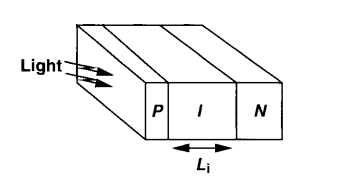
\includegraphics[scale=0.4]{Imagens/PIN.png}
	\end{center}
	\legend{Fonte: \cite{RazaviOpt}}
\end{figure}

Quando um fóton com energia suficiente para excitar o material \'e absorvido, um par el\'etron-lacuna \'e gerado (migração de um el\'etron da banda de valência para de condução), e por difusão, os el\'etrons migram para o cátodo, formando uma fotocorrente. Ajustando-se os tamanhos das camadas P, N e da região de depleção (formada pelo semicondutor intrínseco), podemos controlar a resposta em frequência do fotodiodo e qual a energia mínima do fóton necessária para que gere a fotocorrente. Com a migração dos el\'etrons, uma diferença de potencial \'e gerada entre as camadas P e N, que pode ser aproveitada para a geração de corrente el\'etrica em um circuito el\'etrico fechado \cite{hamamatsu}.
Um fotodiodo apresenta um modelo el\'etrico equivalente ilustrado na \autoref{fig_modelofotodiodo}:

\begin{figure}[!h]
	\caption{\label{fig_modelofotodiodo}Modelo el\'etrico de um fotodiodo}
	\begin{center}
	    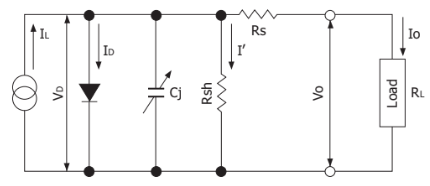
\includegraphics[scale=0.5]{Imagens/ModeloFotodiodo.png}
	\end{center}
	\legend{Fonte: \cite{hamamatsu}}
	\label{modeloElFotodiodo}
\end{figure}

    O modelo el\'etrico apresenta a seguinte expressão:

\begin{equation}
    \label{eq_modEletFot}
    I_o = I_L - I_D - I\rq = I_L - I_S*(\exp (\frac{qV_d}{kT})-1) - I\rq
\end{equation}

Onde:
\begin{itemize}
    \item \textit{I\textsubscript{o}} \'e a corrente de saída presente na carga [\textit{A}]
    \item \textit{V\textsubscript{o}} \'e a tensão de saída [\textit{V}]
    \item \textit{R\textsubscript{L}} \'e a carga de saída [\textit{$\Omega$}]
    \item \textit{V\textsubscript{D}} \'e a tensão presente no diodo do modelo el\'etrico equivalente [\textit{V}]
    \item $I_L$ \'e a corrente fotogerada pela fonte luminosa[\textit{A}]
    \item  \textit{I\textsubscript{D}} \'e a corrente de escuro do fotodiodo (sem a presença de luz) [\textit{A}]
    \item \textit{C\textsubscript{j}} \'e a capacit\^ancia de junção [\textit{F}]
    \item \textit{R\textsubscript{sh}} \'e a resist\^encia shunt do modelo el\'etrico equivalente [$\Omega$]
    \item \textit{I\rq} \'e a corrente shunt presente na resistência shunt do modelo el\'etrico equivalente [\textit{A}]
    \item \textit{R\textsubscript{S}} \'e a resistência em s\'erie com a carga de saída do modelo el\'etrico equivalente [$\Omega$]
    \item \textit{q} \'e a carga el\'etrica de um el\'etron [\textit{C}],
    \item \textit{k} \'e a constante de Boltzmann [\textit{J.K$^{-1}$}],
    \item \textit{T} \'e a temperatura presente no fotodiodo [\textit{K}]
\end{itemize}

O fotodiodo em uma grande faixa apresenta comportamento linear, e \'e a faixa de principal interesse em aplicações como o APS ou o TIA. Com o aumento do n\'umero de f\'otons recebidos, o n\'ivel de corrente tende a ficar cada vez mais negativo, como mostrado na \autoref{fig_respFotodiodo}. Com o aumento ou diminuição expressiva, o circuito começa a se tornar não-linear.

\begin{figure}[!h]
	\caption{\label{fig_respFotodiodo}Resposta Tensão x Corrente para dada intensidade luminosa no fotodiodo}
	\begin{center}
	    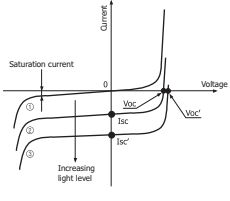
\includegraphics[scale=0.8]{Imagens/graficoRespostaFotodiodo.png}
	\end{center}
	\legend{Fonte: \cite{hamamatsu}}
\end{figure}

\subsection{Figuras de M\'erito}
Do fotodiodo podemos extrair diversas m\'etricas (Figuras de M\'erito), que são de interesse para comparar diferentes modelos. As principais Figuras de M\'erito encontradas na literatura são descritas abaixo, apresentadas em \cite{LidianeCampos}.

\subsubsection{Eficiência Quântica}
Relação entre o número de portadores detectados nos terminais das camadas PN do fotodetector, dividido pela incidência de uma determinada quantidade de fótons no fotodetector.

\begin{equation}
    \eta = \frac{N_e}{N_p}
\end{equation}

Onde:
\begin{itemize}
    \item \textit{$\eta$} \'e Efici\^encia Qu\^antica [\textit{Adm.}]
    \item \textit{N$_e$} \'e o n\'umero de portadores que podem ser detectados nos terminais externos do fotodetector [\textit{n° portadores}]
    \item \textit{N$_p$} incid\^encia de determinada quantidade de f\'otons [\textit{n° f\'otons}]
\end{itemize}

\subsubsection{Responsividade}
Razão entre a corrente fotogerada e a potência óptica incidida no fotodiodo.

\begin{equation}
    \label{eq_responsividade}
    R_\lambda = \frac{I_{PH}}{P_{FD}}
\end{equation}

Onde:
\begin{itemize}
    \item \textit{R$_\lambda$} \'e a Responsividade [\textit{A.W$^{-1}$}]
    \item \textit{I$_{PH}$} \'e a corrente fotogerada [\textit{A}]
    \item \textit{P$_{FD}$} \'e a potência \'optica presente no fotodiodo [\textit{W}]
\end{itemize}

A Eficiência Quântica e a Responsividade se relacionam de acordo com a \autoref{eqEfResp}.

\begin{equation}
    \label{eqEfResp}
    R_\lambda = \frac{\lambda\eta}{1,24}
\end{equation}

Onde:
\begin{itemize}
    \item \textit{R$_\lambda$} \'e a Responsividade [\textit{A.W$^{-1}$}]
    \item $\lambda$ \'e o comprimento de onda da luz incidente [\textit{m}]
    \item $\eta$ \'e Efici\^encia Qu\^antica [\textit{Adm.}]
\end{itemize}

A \autoref{fig_eqEfResp} mostra o gráfico da Responsividade e Efici\^encia Qu\^antica de alguns materiais.

\begin{figure}[!h]
	\caption{\label{fig_responsividade}Responsividade e Efici\^encia Qu\^antica dos materiais Ge, InGaAs, Si}
	\begin{center}
	    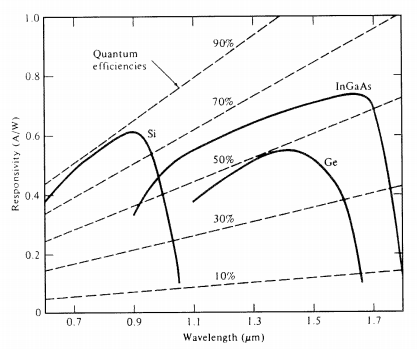
\includegraphics[scale=0.5]{Imagens/GraficoRespostaEspectral.png}
	\end{center}
	\legend{Fonte: \cite{ajoy}}
	\label{fig_eqEfResp}
\end{figure}


\subsubsection{Velocidade de Resposta}
A velocidade de resposta indica o quão rápido o fotodiodo \'e capaz de responder a estímulos de luz externos, em determinada frequência. É caracterizado pelo Tempo de Subida e Tempo de Descida do Fotodiodo, na faixa de frequências de interesse.

O Tempo de Subida \'e calculado como o tempo do qual um fotodiodo, inicialmente sem incidência de luz, leva para elevar o seu nível de tensão nos seus terminais de 10\% para 90\% do seu pico, a partir do no momento que começar a absorver fótons de uma fonte luminosa controlada, em determinada frequência.

O Tempo de Descida \'e calculado como o tempo do qual um fotodiodo, inicialmente com determinada incidência de luz e já estabilizado na sua respectiva tensão de pico, leva para diminuir a diferença de tensão entre seus terminais de 90\% para 10\% do seu pico, a partir do momento que não absorve mais fótons de origem de uma fonte luminosa controlada, em determinada frequência.

\begin{figure}[!h]
	\caption{\label{fig_velocidadeResp}Representação gr\'afica do Tempo de Subida e Descida}
	\begin{center}
	    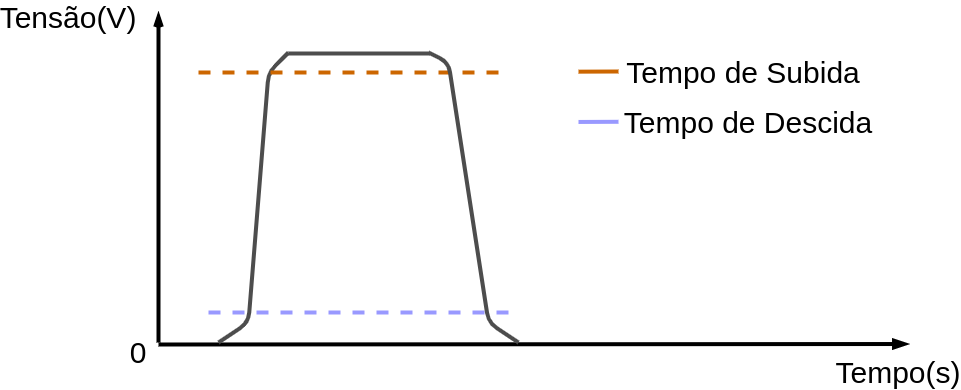
\includegraphics[scale=0.3]{Imagens/GraficoVelocidadeResposta.png}
	\end{center}
	\legend{Fonte: Produzido pelo autor}
\end{figure}

O conhecimento da velocidade de resposta \'e crucial para determinar as limitações do projeto em termos de processamento de informações. A amostragem de dados deve ter período maior do que os tempos de subida e de descida do fotodiodo, nos maiores valores apresentados na faixa de frequência desejada.

\subsubsection{Resposta Espectral}

O Efeito Fotoel\'etrico se caracteriza pela excitação de el\'etrons em um material por um fóton, quando este apresenta uma energia mínima, chamada de \textit{Função Trabalho}. Mesmo quando uma grande quantidade de fótons com energia menor do que a Função Trabalho atravessem o fotodiodo, eles não serão capazes de excitar nenhum el\'etron. Como a energia de um fóton diminui com o aumento de seu comprimento de onda, existe um comprimento de onda máximo (ou uma frequência mínima) do qual o fotodetector será capaz de gerar fotocorrente.

Por outro lado, uma diminuição do comprimento de onda tende a excitar cada vez menos el\'etrons, pois a absorção na região de depleção deixa de acontecer, chegando a um ponto que o fotodiodo sature em resposta e não seja mais possível diferenciar diferentes frequências acima desta.
Sabendo destas limitações, definimos a Resposta Espectral como a faixa de comprimentos de onda do qual o fotodetector \'e capaz de produzir uma fotocorrente correspondente.

\subsubsection{Relação Sinal-Ruído}
Razão entre a potência de sinal fotogerada pela pot\^encia de ru\'ido no sinal.

\begin{equation}
    SNR = \frac{P_{SINAL}}{P_{Ru\acute{i}do}}
\end{equation}

Onde:
\begin{itemize}
    \item \textit{SNR} \'e relação sinal-ru\'ido [\textit{Adm.}]
    \item \textit{P\textsubscript{SINAL}} \'e a pot\^encia do sinal fotogerado [\textit{W}]
    \item \textit{V\textsubscript{D}} \'e a pot\^encia do ruido do sinal fotogerado [\textit{W}]
\end{itemize}

\subsubsection{Pot\^encia equivalente ao ru\'ido}
Pot\^encia da luz incidida no fotodiodo, que gera uma potência de sinal equivalente ao de ruído em largura de 1 Hz

\begin{equation}
    NEP = P_{Ru\acute{i}do 1 H}
\end{equation}

Onde:
\begin{itemize}
    \item \textit{NEP} \'e a pot\^encia da luz incidida no fotodiodo [\textit{W}]
    \item \textit{P\textsubscript{Ruído 1 Hz}} \'e a potência do ruído em largura de 1 Hz [\textit{W}]
\end{itemize}

\subsubsection{Detectividade espec\'ifica}
Razão entre a raiz quadrada da área fotossensível do diodo, sobre o NEP

\begin{equation}
    D* = \frac{\sqrt{A.B}}{NEP}
\end{equation}

Onde:

\begin{itemize}
    \item \textit{D*} \'e a detectividade espec\'ifica [$cm.\sqrt{Hz}.W^{-1}$]
    \item \textit{A} \'e a \'area da região fotossens\'ivel do fotodiodo [\textit{cm²}]
    \item \textit{A} \'e a largura de banda [\textit{Hz}]
\end{itemize}

\section{Sensor de Pixel Ativo (APS)}
\label{section:APS}
Um APS \'e um dispositivo do qual se aproveita das características de um fotodiodo para gerar um sinal que pode ser amostrado e então quantificado, de forma a produzir informações referentes à luz incidida no fotodetector.

Dentre as várias possibilidades de produção de um circuito APS, aquele estudado ao longo de todo este trabalho se apresenta na \autoref{fig_APS}.

\begin{figure}[!h]
	\caption{\label{fig_APS}Circuito APS do trabalho}
	\begin{center}
	    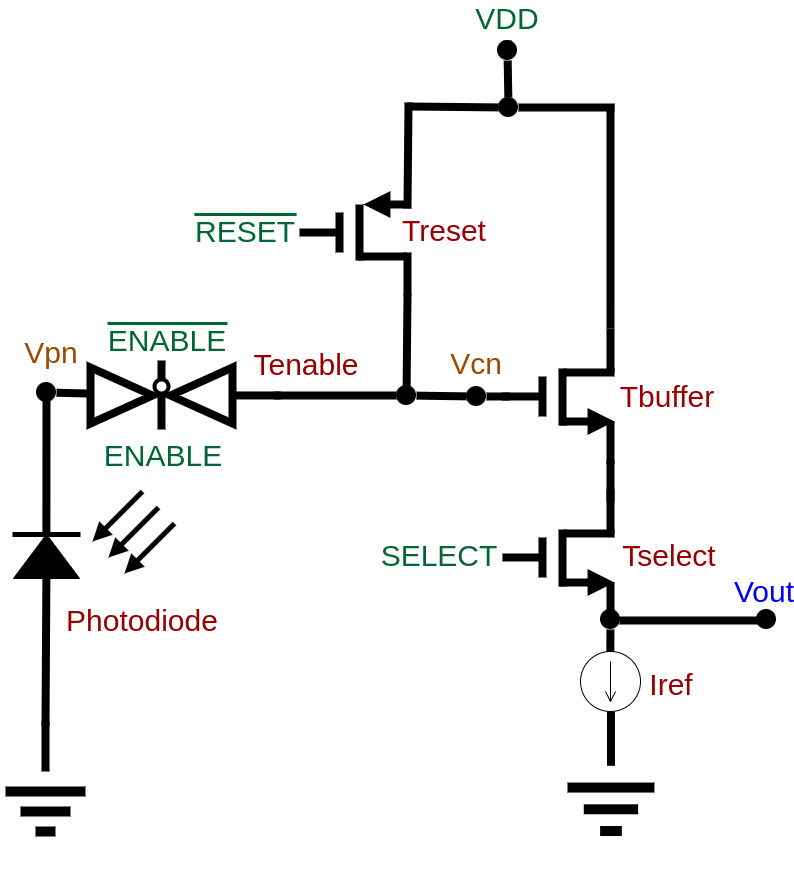
\includegraphics[scale=0.3]{Circuitos/APS.png}
	\end{center}
	\legend{Fonte: Produzido pelo autor}
\end{figure}

Cada componente desempenha uma diferente função de forma a processar a informação advinda da corrente fotogerada:

\begin{itemize}

    \item O transistor $T_{buffer}$ funciona como um amplificador de Dreno Comum, e seu papel \'e replicar o sinal advindo do n\'o central ao n\'o de sa\'ida, reduzindo o efeito de carga que aconteceria caso o n\'o central ($V_{cn}$) fosse a saída do sistema.

    \item O transistor $T_{reset}$ funciona como uma chave, que quando fechada (nível lógico '0' em seu gate), vale VDD. Quando aberto (nível lógico '1' em seu gate), o sinal no n\'o central passa a depender da configuração da Porta de Transmissão.

    \item A Porta de Transmissão $T_{enable}$ funciona como uma chave, e quando o transistor $T_{reset}$ estiver em aberto, tem a função controlar se a tensão presente no fotodiodo ir\'a para o nó central ou não. Quando aberto, $V_{pn}$ fica isolado do restante do circuito, devido ao estado de alta imped\^ancia nos terminais do dispositivo. Quando fechado, a corrente fotogerada descarrega em $V_{cn}$, pois a associação das capacitâncias parasitas presentes nos transistores de $T_{enable}$, $T_{reset}$ e $T_{buffer}$ formam um caminho fechado do qual descarrega lentamente o fotodiodo \cite{LidianeCampos}. Uma representação desses capacitores \'e dada na \autoref{fig_APS_cap}.
    
    \item O transistor $T_{select}$ \'e utilizado para que m\'ultiplos APS's compartilhem um mesmo barramento de sa\'ida. No projeto aqui implementado $T_{select}$ sempre se apresentar\'a fechado (\textit{SELECT} em n\'ivel l\'ogico '1').
    
    \item A fonte de corrente \textit{$I_{ref}$} tem a função de polarizar a sa\'ida do circuito, além de aprimorar a linearidade do estágio de sa\'ida \cite{RazaviFundM}.

\end{itemize}

    H\'a dois n\'os internos de bastante interesse ao trabalho, que são:

\begin{itemize}
    \item \textit{$V_{pn}$}: tensão entre os terminais do fotodiodo [\textit{V}]
    \item \textit{$V_{cn}$}: tensão no n\'o central do APS [\textit{V}]
\end{itemize}

    Os sinais externos do circuito são:
    
\begin{itemize}
    \item \textit{RESET}: fecha o transistor $T_{reset}$. Ativo em n\'ivel l\'ogico '0'.
     \item \textit{SELECT}: fecha o transistor $T_{select}$. Ativo em n\'ivel l\'ogico '1'. No circuito do trabalho estar\'a sempre configurado como '1'.
     \item \textit{ENABLE}: fecha o transmition gate $T_{enable}$. Ativo em n\'ivel l\'ogico '1'.
     \item \textit{VDD}: Alimentação do circuito
\end{itemize}

\subsubsection{Capacit\^ancias Parasitas}
Para o correto estudo do APS devemos observar a capacit\^ancia equivalente $C_{eq}$ presente nos n\'os $V_{pn}$ e $V_{cn}$ do circuito \cite{LidianeCampos}. Na \autoref{fig_APS_cap} temos uma representação das capacit\^ancias que compõem $C_{eq}$.

\begin{figure}[!h]
	\caption{\label{fig_APS_cap}Representação do circuito APS com suas capacit\^ancias parasitas destacadas}
	\begin{center}
	    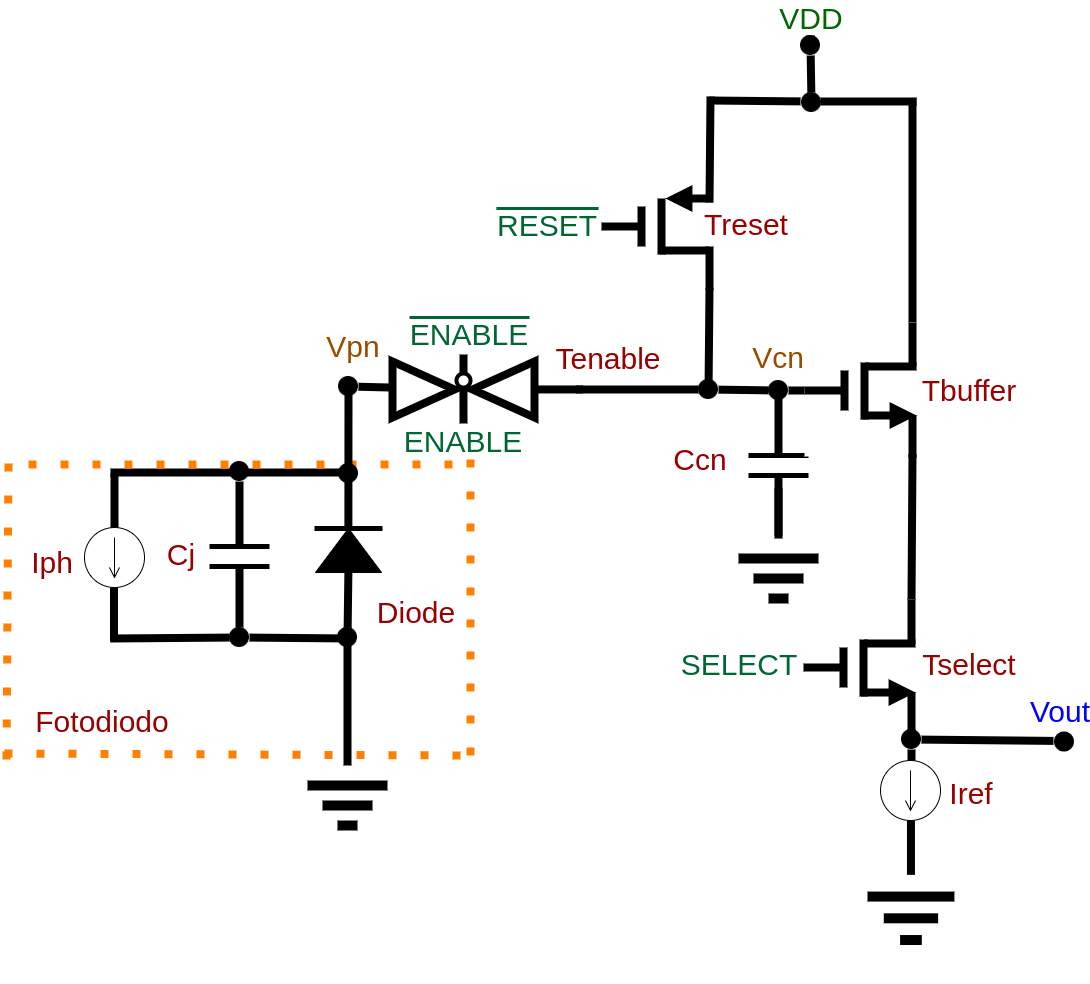
\includegraphics[scale=0.3]{Circuitos/APS_cap.png}
	\end{center}
	\legend{Fonte: Produzido pelo autor}
\end{figure}

Onde: 

\begin{itemize}
    \item $C_j$ \'e a capacit\^ancia de junção do fotodiodo. Seu principal efeito no estudo do APS \'e limitar a velocidade de varia ão da corrente fotogerada.
    
    \item $C_{cn}$ \'e a capacit\^ancia equivalente vista do n\'o $V_{cn}$ ao GND, devido principalmente às capacit\^ancias presentes em $T_{enable}$,  $T_{reset}$ e $T_{buffer}$, sendo o de $T_{buffer}$ o de maior contribuição. O capacitor cria um caminho fechado para a corrente do fotodiodo circular ao GND e ser descarregado em um dos est\'agios citados posteriormente no trabalho.
    
    \item $I_{ph}$ \'e a corrente fotogerada [\textit{A}].
    
    \item \textit{Diodo} \'e o diodo do modelo el\'etrico equivalente do fotodiodo.
\end{itemize}

\subsubsection{Est\'agios}
\label{estagiosAPS}

A operação do APS pode ser dividida em 4 est\'agios, que vão definir os m\'inimos momentos de  atuação no sinal de controle e seus limites operação. Os est\'agios são representados na \autoref{figura_estagiosAPS}, tendo como base o trabalho de \cite{LidianeCampos}.

\begin{figure}[!h]
	\caption{\label{figura_estagiosAPS}Esboço de resposta do APS ao controlar seus sinais de entrada}
	\begin{center}
	    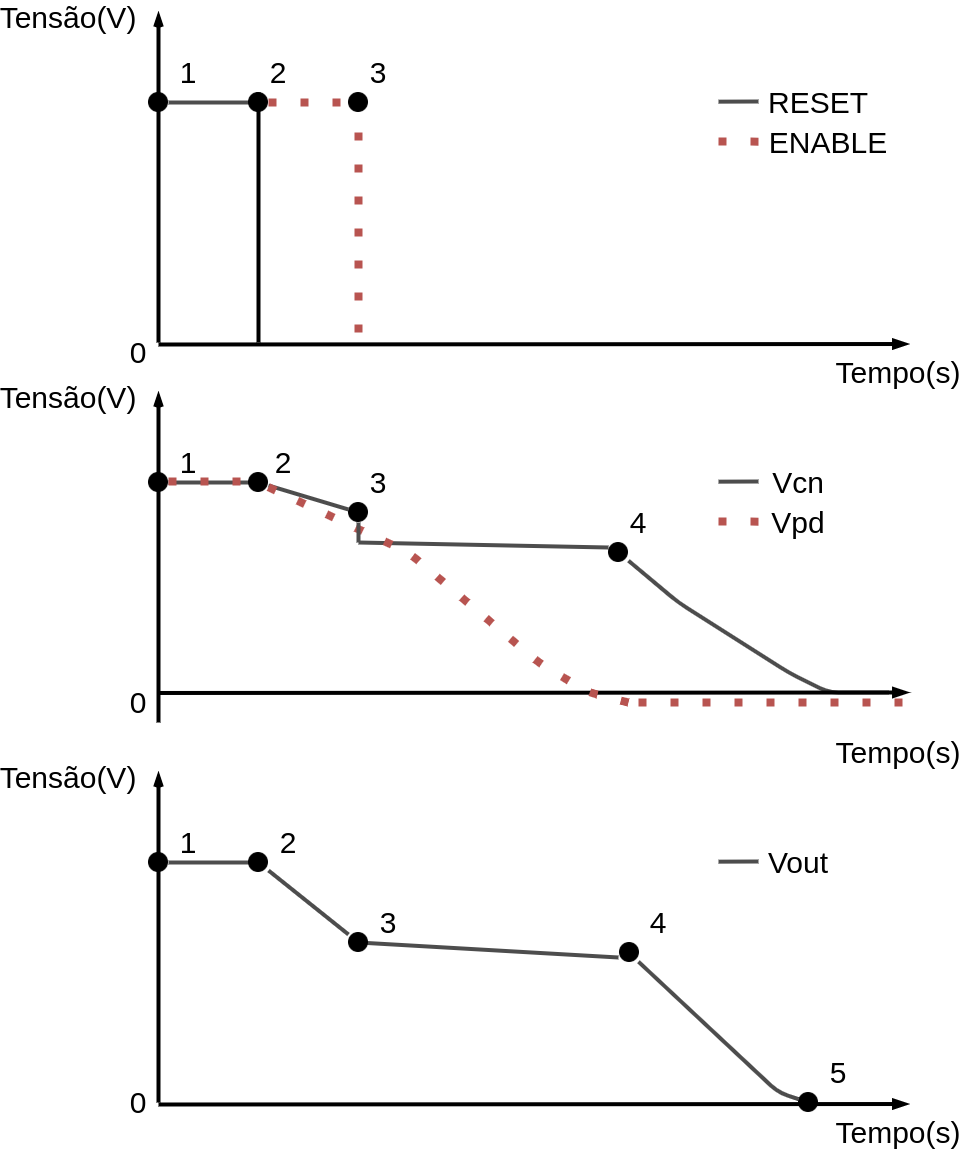
\includegraphics[scale=0.2]{Imagens/estagiosAPS.png}
	\end{center}
	\legend{Fonte: Adaptado de \cite{LidianeCampos}}
\end{figure}

\begin{enumerate}

\item $T_{reset}$ fechado, $T_{enable}$ fechado (Período de Reset)
    
Nessa condição, o n\'o $V_{cn}$ \'e igual a VDD.

\item $T_{reset}$ aberto, $T_{enable}$ fechado (Período de Integração)

A corrente fotogerada passa a descarregar a capacit\^ancia $C_{cn}$ do nó central. A tensão no fotodiodo passa a diminuir, devido a circulação de corrente que diminui a carga de $C_{j}$.

A tensão $V_{cn}$ neste segundo est\'agio tem uma relação linear com a corrente fotogerada, conforme descrito na \autoref{eq_modEletFotIl}, que \'e deduzida fazendo an\'alises dos n\'os, desprezando-se a resistência presente em $T_{enable}$ e também outras resistências parasitas, como aquelas presentes no modelo elétrico do fotodiodo apresentado na \autoref{modeloElFotodiodo}.

\begin{equation}
    \label{eq_modEletFotIl}
    V_{cn}(t) = V_0-\frac{I_{PH}}{C_j+C_{cn}}t
\end{equation}

Onde:

\begin{itemize}
    \item $V_{cn}(t)$ \'e a tensão do nó $V_{cn}$ em determinado tempo $t$ [$V$]
    \item $V_0$ \'e a tensão do nó $V_{cn}$ no momento que o estágio inicia. Comumente deseja-se que esta tensão seja a máxima possível [$V$]
    \item $I_{PH}$ \'e a corrente fotogerada [$A$]
    \item $C_j$ \'e a capacit\^ancia de junção do fotodiodo [$F$]
    \item $C_{cn}$ \'e a capacit\^ancia do n\'o central do APS [$F$]
    \item $t$ \'e o tempo a partir do qual o estágio se iniciou [$s$]
\end{itemize}

Já a tensão de saída $V_{out}$ é dada pela \autoref{eq_voutaps}, que junto a \autoref{eq_modEletFotIl} resulta na \autoref{eq_voutfinal}, utilizada no trabalho para calcular a tensão de saída do APS em determinado instante de tempo do Estágio 2.

\begin{equation}
    \label{eq_voutaps}
    V_{out}(t) = V_{cn} - V_{GS\_buffer}
\end{equation}

\begin{equation}
    \label{eq_voutfinal}
    V_{out}(t) = V_0-\frac{I_{PH}}{C_j+C_{cn}}t - V_{GS\_buffer}
\end{equation}

Onde:

\begin{itemize}
    \item $V_{out}(t)$ \'e a tensão de saída do APS em determinado tempo $t$ [$V$]
    \item $V_{GS\_buffer}$ \'e a diferença de potencial entre $V_{cn}$ e $V_{out}(t)$, que considerando-se a ausência de efeitos de carga, e que $T_{buffer}$ esteja sempre na região de saturação no Estágio 2, é uma constante [$V$]
\end{itemize}

\item $T_{reset}$ aberto, $T_{enable}$ aberto, potencial \textit{$V_{pd}$} positivo

Logo ap\'os abrir o $T_{enable}$, a fotocorrente não circula mais no n\'o central, e o fotodiodo continua a ter sua diferença de potencial reduzida, com circulação de corrente internamente devido a $C_j$. O n\'o central passa a cair bem lentamente devido a correntes de fuga. \textit{$V_{pd}$} cai at\'e chegar a se tornar negativo;

\item \textit{$T_{reset}$} aberto, \textit{$T_{enable}$} aberto, potencial \textit{$V_{pd}$} negativo

Nessa situação, o $T_{enable}$ passa a operar em modo linear. O potencial no n\'o $V_{cn}$ passa a cair devido a circulação de corrente do n\'o at\'e o fotodiodo. O nó diminui at\'e que finalmente chega a 0, onde se mant\'em estável e não apresenta mais circulação de corrente.

\end{enumerate}

\subsection{Amostrando informações da luz com um APS básico}
\label{secao_amostrando}

Podemos aproveitar o entendimento das propriedades f\'isicas do fotodiodo, e tamb\'em dos est\'agios de funcionamento de um APS, para obtermos informações relativas aos f\'otons absorvidos.

Como sabemos matematicamente as relações de fotocorrente determinadas por \autoref{eq_modEletFot} e \autoref{eq_modEletFotIl}, e tamb\'em as Figuras de M\'erito que caracterizam o fotodetector, podemos utilizar o APS para coletar as informações em sua sa\'ida e determinar a intensidade da luz

Entre os est\'agios 2 e 3, a tensão do n\'o $V_{cn}$ passa a cair, devido a circulação da fotocorrente. Como essa corrente depende da intensidade da luz, podemos descobrir o valor de intensidade sabendo a inclinação da curva de tensão na sa\'ida, j\'a que a variação da tensão \'e uma grandeza diretamente proporcional à corrente e a imped\^ancia vista no n\'o. Como a tensão de sa\'ida \'e igual ao de $V_{cn}$ menos $V_{GS}$ do transistor $T_{buffer}$, podemos medir a sa\'ida para processar o sinal e então relatar a intensidade luminosa.

Com as observações aqui apresentadas, podemos desenvolver um sistema de medição de informação luminosa, trabalhando entre os est\'agios 1 e 3, e então retornando ao Estágio 1 para uma nova aquisição. \'E importante destacar que existem limitações quanto \`a temporização dos est\'agios. Para que a medição seja realizada de forma adequada, devemos garantir que tenhamos entre o Est\'agio 1 e 2, um tempo suficientemente grande para que $V_{cn}$ apresente um valor estável, ou seja, o tempo de transição do sistema nessa condição seja conclu\'ido. Entre o Est\'agio 2 e Est\'agio 3, devemos garantir que tenhamos um tempo mínimo para que dois valores distintos de $V_{out}$ possam ser medidos, de acordo com a sensibilidade do sistema de medição.

\section{Amplificador de Transimped\^ancia (TIA)}
\label{section:TIA}

Um amplificador de transimped\^ancia \'e um circuito em que dada uma corrente de entrada, gera-se uma tensão em sua sa\'ida proporcional \`a esta corrente \cite{RazaviFundM}. Considerando-se o fotodiodo como uma fonte de corrente, a \autoref{fig_TIA} apresenta uma poss\'ivel topologia de um TIA, desenvolvido no presente trabalho.

\begin{figure}[!h]
	\caption{\label{fig_TIA}TIA desenvolvido}
	\begin{center}
	    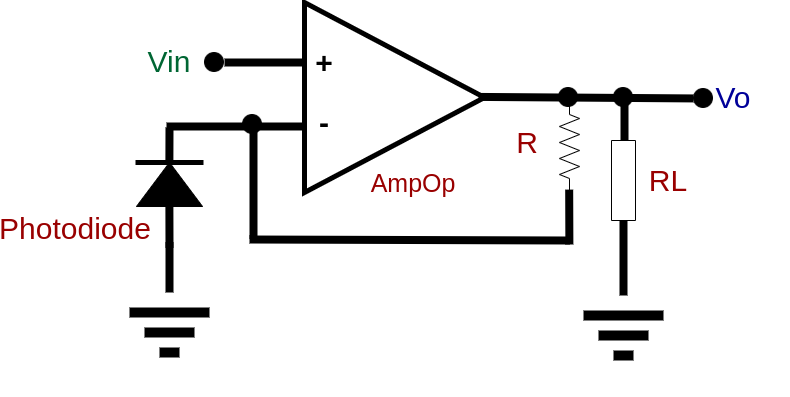
\includegraphics[scale=0.3]{Circuitos/TIA.png}
	\end{center}
	\legend{Fonte da ilustra ão: Pr\'oprio autor}
\end{figure}

Onde:

\begin{itemize}
    \item $V_{ref}$ \'e a tensão de entrada de referência [$V$]
    \item $V_o$ \'e a tensão de sa\'ida [$V$]
    \item $R$ \'e uma resist\^encia de ajuste ganho [$\Omega$]
    \item $R_l$ \'e uma carga de sa\'ida [$\Omega$]
\end{itemize}

Sabemos da \autoref{fig_modelofotodiodo} que podemos modelar uma resist\^encia $R_{sh}$ em paralelo ao fotodiodo. Desprezando-se todos outros componentes do modelo para facilitar a an\'alise, podemos descrever a f\'ormula correspondente ao $TIA$ como a \autoref{eqCTIA}.

\begin{equation}
    \label{eqCTIA}
    V_o = RI_{PH} + (1+\frac{R}{R_{sh}})V_{ref}
\end{equation}

Onde:
\begin{itemize}
    \item $I_{PH}$ \'e a corrente fotogerada [$A$]
\end{itemize}

A \autoref{eqCTIA} nos mostra que \textit{R} deve ser ajustado de forma que não seja grande demais, pois valores altos (de acordo com a aplicação) irão gerar tensão na sa\'ida com variação muito grande. Mesmo que Vref fosse colocado em GND, o fator $(1+\frac{R}{R_{sh}})$ ainda pode dominar a relação, devido \'a ruídos presentes no nó, e então impor um termo indesejado, o que também causaria problemas quando \textit{R} fosse muito alto \cite{hamamatsu}.

Devido ao produto $RI_{PH}$, também devemos ter o cuidado de não tornar \textit{R} pequeno demais para que tenhamos a sensibilidade no sinal de saída de forma adequada.

Considerando $R_{sh} >> R$, chegamos à \autoref{eqCTIA2}, utilizada no projeto apresentado no trabalho.

\begin{equation}
    \label{eqCTIA2}
    V_o = RI_{PH}
\end{equation}

\subsection{Resposta espectral de um TIA}

Como a imped\^ancia de entrada do $TIA$ não \'e ideal (infinita) e varia com a frequ\^encia e temperatura, o circuito não se apresenta linear em toda sua banda de operação, o que representa uma variação na resposta em frequ\^encia de acordo com a corrente fotogerada \cite{hamamatsu}.
Como o pr\'oprio amplificador apresenta capacit\^ancias internas, o circuito \'e tamb\'em limitado em altas frequ\^encias, principalmente pelo produto $R$ vezes $C$, onde C \'e a capacit\^ancia interna vista pelos terminais de $R$ \cite{hamamatsu}.

Dada as duas propriedades, a \autoref{figura_respostaTIA} e a \autoref{figura_respostaTIA2} mostram o comportamento t\'ipico de resposta em frequ\^encia da topologia.

\begin{figure}[!h]
 \centering
    \centering
    \caption{\label{figura_respostaTIA}Resposta espectral de um TIA}
	\begin{center}
	    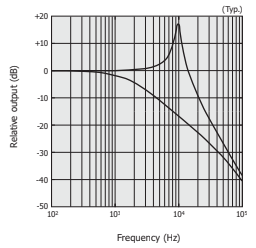
\includegraphics[scale=0.8]{Imagens/RespostaEspectralTIA.png}
	\end{center}
	\legend{Fonte: \cite{hamamatsu}}
\end{figure}

\begin{figure}[!h]
    \centering
    \caption{\label{figura_respostaTIA2}Resposta a um pulso em um TIA}
	\begin{center}
	    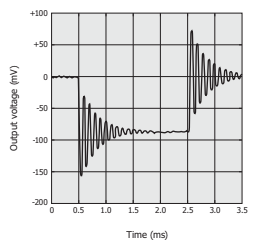
\includegraphics[scale=0.8]{Imagens/RespostaEspectralTIA2.png}
	\end{center}
	\legend{Fonte: \cite{hamamatsu}}
\end{figure}

% ----------------------------------------------------------
% PARTE
% ----------------------------------------------------------
\part{Projeto}
% ----------------------------------------------------------
\chapter[Desenvolvimento do Projeto]{Desenvolvimento do Projeto}

O capítulo apresenta o projeto realizado nesta dissertação, contendo a explicação do que foi desenvolvido, os circuitos esquemáticos, e os parâmetros dos componentes. Alguns circuitos não foram incluídos neste capítulo e são apresentados de maneira implícita, devido à sua simplicidade, flexibilidade de implementação em replicações do trabalho, e o autor também entende que os mesmos já são de amplo conhecimento na área. No \autoref{blocosadicionais} é possível verificar mais sobre esses blocos e como foram desenvolvidos, caso o leitor sinta a necessidade de entender a sua implementação.

\newcommand{\NomeBloco}{NULL}
\newcommand{\NomeBlocoNoIt}{NULL}
\newcommand{\NomeBlocoNoUnderline}{NULL}
\newcommand{\NomePTab}{tab_\NomeBlocoNoUnderline}
\newcommand{\NomeSTab}{tab_\NomeBlocoNoUnderline2}
\newcommand{\NomePFig}{fig_\NomeBlocoNoUnderline}
\newcommand{\NomeSFig}{fig_\NomeBlocoNoUnderline2}
\newcommand{\NomeTTab}{tab_\NomeBlocoNoUnderline3}
\newcommand{\NomeQTab}{tab_\NomeBlocoNoUnderline4}

Um circuito integrado foi desenvolvido para avaliar cinco dispositivos APS's, referenciado na se{\c c}\~ao \ref{section:APS} deste documento, e dois TIA's, em refer\^encia \`a se{\c c}\~ao \ref{section:TIA}. O projeto \'e representado em alto n\'ivel na \autoref{fig_circcompleto}. Todos os sinais aqui apresentados na figura, e tamb\'em em todas figuras \'a seguir, seguem o a padr\~o descrito na se{\c c}\~ao \ref{section:padrao_sinais} deste trabalho.

\begin{figure}[htb]
	\caption{\label{fig_circcompleto}Circuito projetado}
	\begin{center}
	    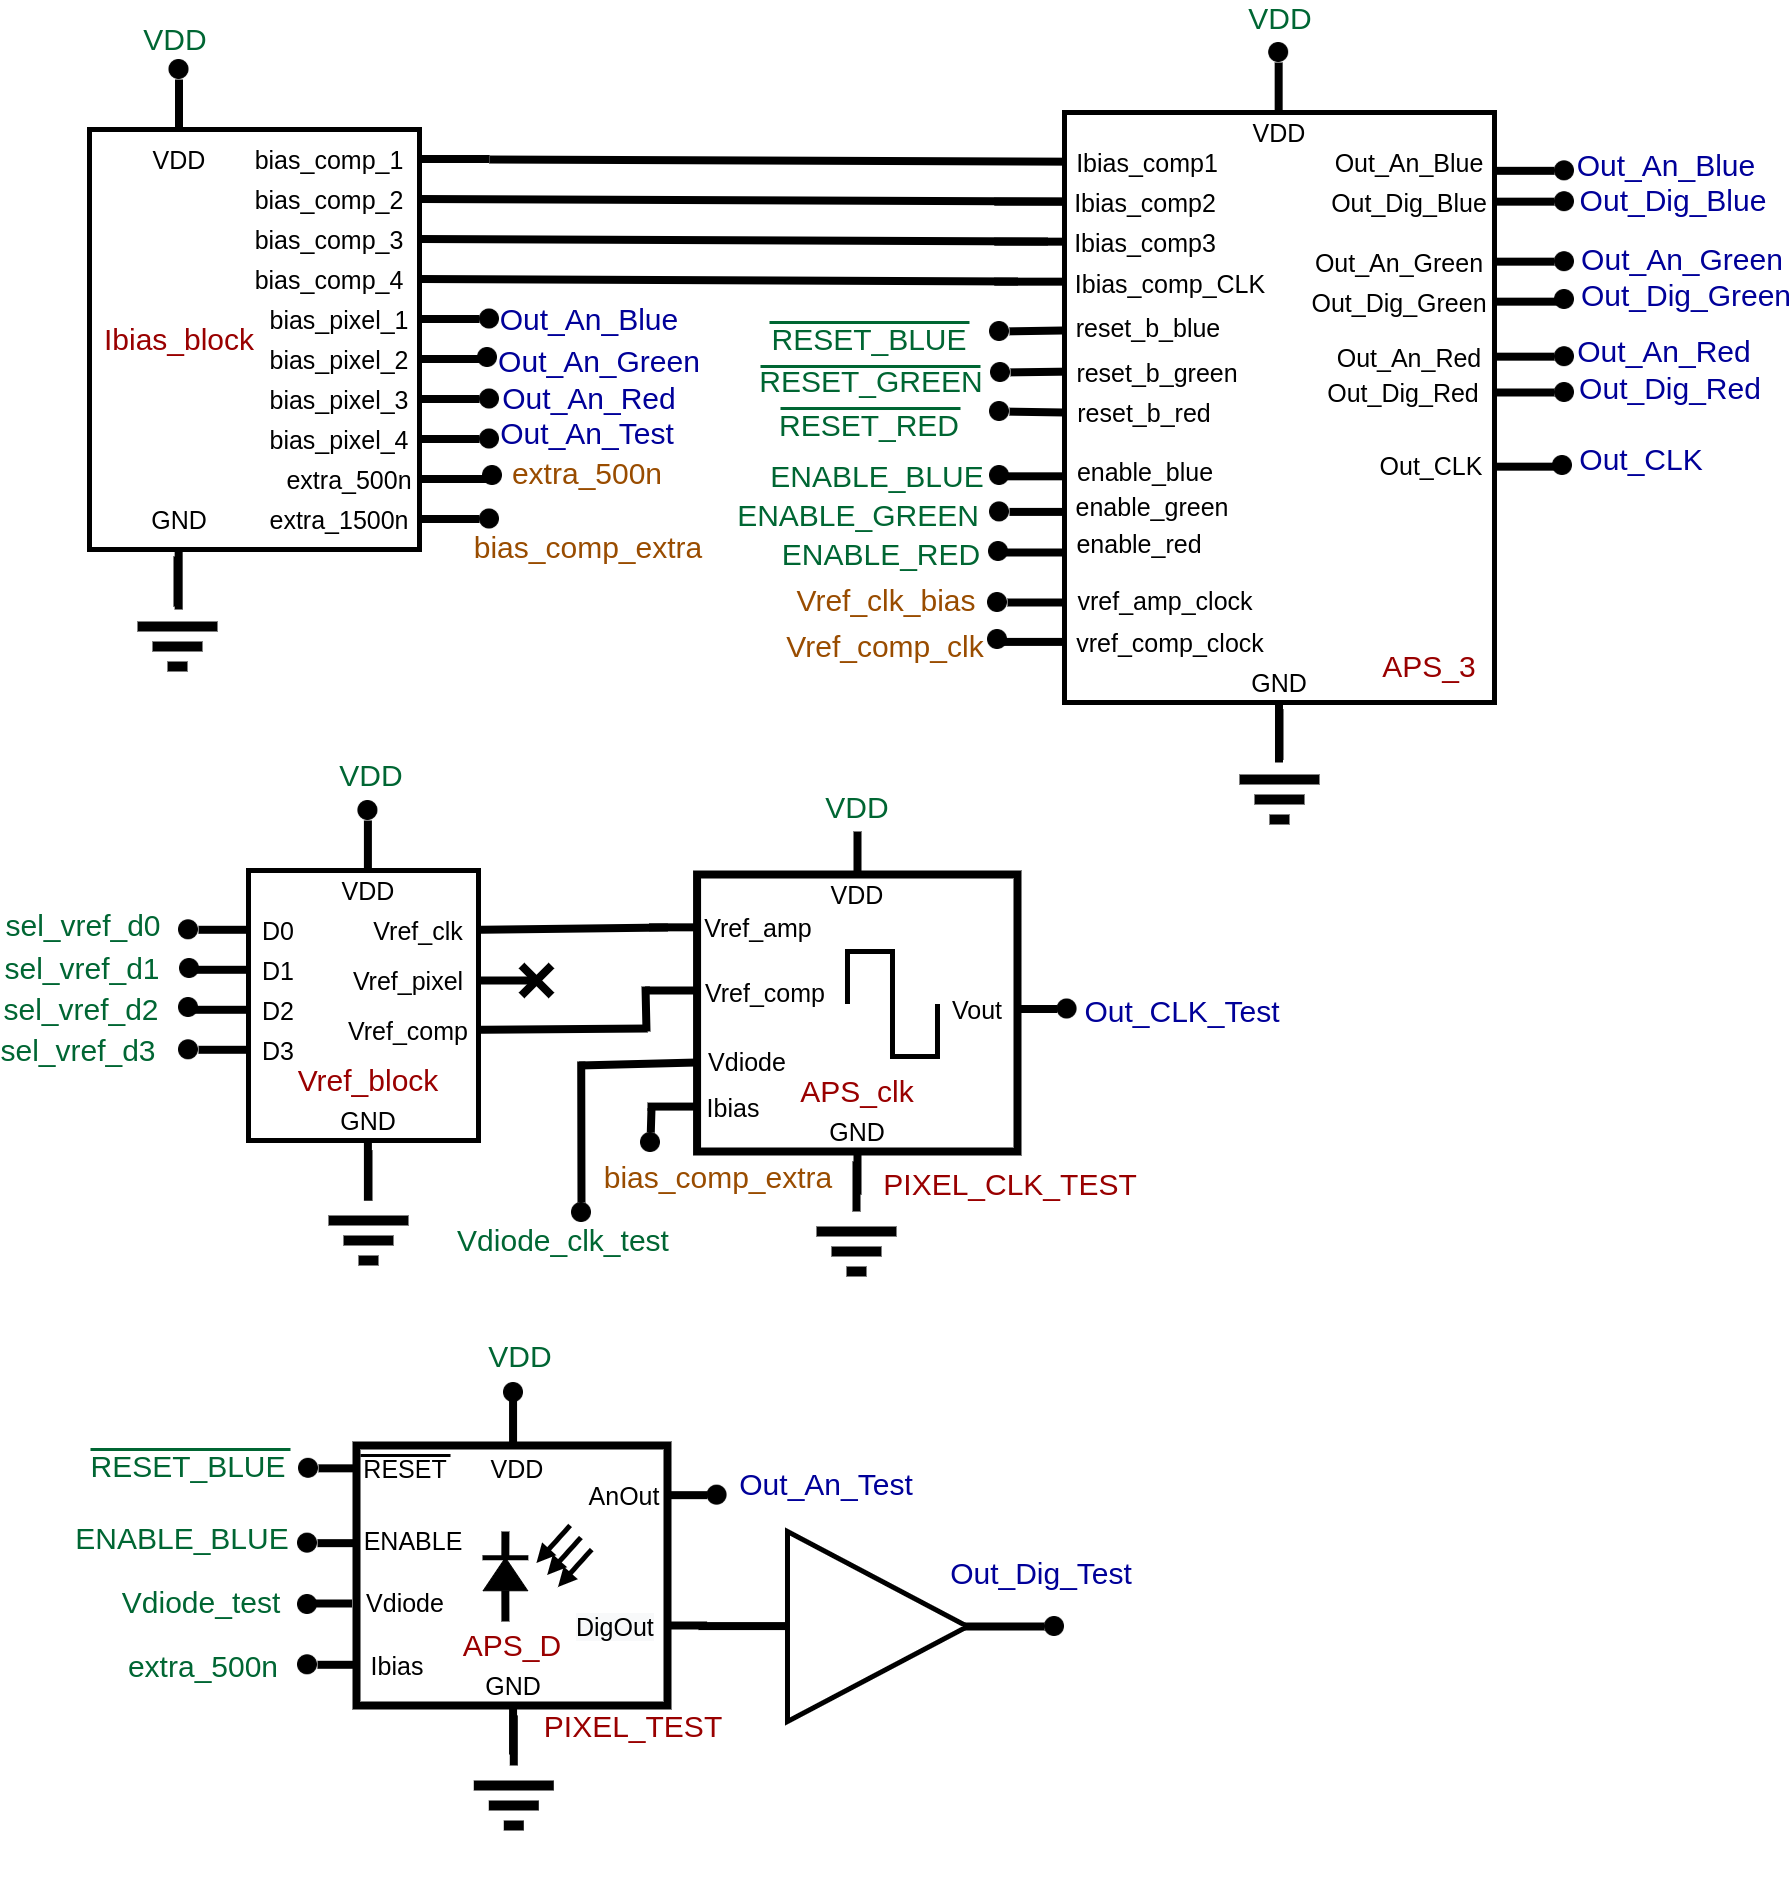
\includegraphics[width=\textwidth]{Circuitos/Complete_Circuit.png}
	\end{center}
	\legend{Fonte: Produzido pelo autor}
\end{figure}

O circuito tem a finalidade de processar a informa{\c c}\~ao advinda de tr\^es APS's, constru\'idos de maneira id\^entica em n\'ivel de layout, com a finalidade de abstrair informa{\c c}\~oes de cores advindas de uma fonte luminosa, dos quais podem ser Azul, Verde ou Vermelha. Para que as cores fossem devidamente separadas entre cada APS, filtros luminosos externo, por meio de uma pel\'icula colorida, s\~ao adicionados sob cada APS respons\'avel por processar uma cor equivalente \`a de sua pel\'icula.

Um sinal luminoso de cor branca tamb\'em \'e utilizado no sistema de forma a ser a refer\^encia de rel\'ogio de todos APS's descritos. Esse sinal \'e processado utilizando-se um $TIA$, do qual \'e gerado um sinal el\'etrico equivalente \'a informa{\c c}\~ao luminosa.

A tecnologia de fabrica{\c c}\~ao utilizada para o desenvolvimento de todos blocos foi a \emph{CMOS 180nm da TSMC}. O software utilizado para o projeto do dispositivo foi o \emph{Virtuoso}, desenvolvido pela \emph{Cadence}.

O circuito representado na \autoref{fig_circcompleto} \'e composto por 2 blocos principais, que permitem o processamento advindos da fonte luminosa, al\'em de um circuito \emph{APS} e um \emph{TIA} extra. A descri{\c c}\~ao dos bloco s\~ao:

\begin{itemize}
    \item \emph{ibias\_block}: Tem a fun{\c c}\~ao de gerar todas fontes de corrente utilizadas em todos os blocos do circuito, quando necess\'ario.
    
    \item \emph{4\_APS}: Implementa os tr\^es circuitos APS descritos, al\'em do circuito \emph{TIA}. A sa\'ida de cada bloco passa por um comparador de forma a digitalizar o dado, como ser\'a melhor explicitado na se{\c c}\~ao \autoref{Bloco4APS}.
    
    \item \emph{Vref\_block} e \emph{PIXEL\_CLK\_TEST}: Estes blocos realizam a implementa{\c c}\~ao de um TIA, por\'em com a adi{\c c}\~ao de um pino extra que possibilita a simula{\c c}\~ao de uma corrente fotogerada sem necessitar de uma fonte luminosa. Estes blocos ser\~ao melhor explicados na se{\c c}\~ao \autoref{BlocoTIA}. 
    
    \item \emph{Vref\_block} e \emph{PIXEL\_TEST}: Este blocos realizam a implementa{\c c}\~ao de um APS, por\'em com a adi{\c c}\~ao de um pino extra que possibilita a simula{\c c}\~ao de uma corrente fotogerada sem necessitar de uma fonte luminosa. Estes blocos ser\~ao melhor explicados na se{\c c}\~ao \autoref{BlocoAPS}.
    
\end{itemize}

A \autoref{tab_circcomp} mostra a rela{\c c}\~ao de sinais de entrada e sa\'ida presentes no circuito, para o processamento dos p\'ixels de cor. A \autoref{tab_circcomp2} mostra a rela{\c c}\~ao de sinais de entrada e sa\'ida presentes no circuito para o processamento dos blocos de teste.

\begin{table}[htb]
\IBGEtab{%
  \caption{Descri{\c c}\~ao dos sinais de entrada e sa\'ida do circuito projetado para as cores azul, verde e vermelha}%
  \label{tab_circcomp}
}{%
  \begin{tabular}{ccll}
  \toprule
   Sinal & Tipo & Descri{\c c}\~ao & Observa{\c c}\~ao \\
  \midrule \midrule
   RESET\_BLUE & Entrada & Sinal de \emph{RESET} no APS para cor azul & Ativo em n\'ivel baixo \\
  \midrule
   RESET\_GREEN & Entrada & Sinal de \emph{RESET} no APS para cor verde & Ativo em n\'ivel baixo \\
  \midrule
   RESET\_RED & Entrada & Sinal de \emph{RESET} no APS para cor vermelha & Ativo em n\'ivel baixo \\
  \midrule
   ENABLE\_BLUE & Entrada & Sinal de \emph{ENABLE} no APS para cor azul & Ativo em n\'ivel alto \\
  \midrule
   ENABLE\_GREEN & Entrada & Sinal de \emph{ENABLE} no APS para cor verde & Ativo em n\'ivel alto \\
  \midrule
   ENABLE\_RED & Entrada & Sinal de \emph{ENABLE} no APS para cor vermelha & Ativo em n\'ivel alto \\
  \midrule
   Out\_An\_Blue & Sa\'ida & Sinal anal\'ogico para cor azul \\
  \midrule
   Out\_Dig\_Blue & Sa\'ida & Sinal digital para cor azul \\
  \midrule
   Out\_An\_Green & Sa\'ida & Sinal anal\'ogico para cor verde \\
  \midrule
   Out\_Dig\_Green & Sa\'ida & Sinal digital para cor verde \\
  \midrule
   Out\_An\_Red & Sa\'ida & Sinal anal\'ogico para cor vermelha \\
  \midrule
   Out\_Dig\_Red & Sa\'ida & Sinal digital para cor vermelha \\
  \bottomrule
\end{tabular}%
}{%
  \fonte{Produzido pelo autor.}
}
\end{table}

\begin{table}[htb]
\IBGEtab{%
  \caption{Descri{\c c}\~ao dos sinais de entrada e sa\'ida do circuito projetado para os blocos de teste}%
  \label{tab_circcomp2}
}{%
  \begin{tabular}{cccc}
  \toprule
   Sinal & Tipo & Descri{\c c}\~ao & Observa{\c c}\~ao \\
  \bottomrule
\end{tabular}%
}{%
  \fonte{Produzido pelo autor.}
}
\end{table}
\section{Espelhos de Corrente}

Espelhos de Corrente foram necess\'arios para o desenvolvimento de diversos blocos contidos no projeto, e ser\~ao especificados nas subse{\c c}\~oes \` seguinte. Uma explica{\c c}\~ao geral sobre o funcionamento e desenvolvimento de espelhos de corrente pode ser visto na \autoref{anexoespelhos}.

\renewcommand{\NomeBloco}{ibias\_generator}
\renewcommand{\NomeBlocoNoUnderline}{ibiasgenerator}
\renewcommand{\NomePTab}{tab_\NomeBlocoNoUnderline}
\renewcommand{\NomeSTab}{tab_\NomeBlocoNoUnderline2}
\renewcommand{\NomePFig}{fig_\NomeBlocoNoUnderline}
\renewcommand{\NomeSFig}{fig_\NomeBlocoNoUnderline2}
\renewcommand{\NomeTTab}{tab_\NomeBlocoNoUnderline3}
\renewcommand{\NomeQTab}{tab_\NomeBlocoNoUnderline4}

\subsection{ibias\_generator}
 
O bloco \NomeBloco{}\footnote{Circuito desenvolvido pelo aluno \textit{Daniel Carvalho Lott}, do curso de bacharelado em Engenharia Elétrica da UFMG, no ano de 2020} \'e um espelho de corrente que apresenta uma sa\'ida de 50 $\mu$A. O bloco apresenta as definições de sinais de entrada e sa\'ida referidos na \autoref{\NomeSTab}.

\begin{table}[htbp]
\caption{Sinais do bloco \NomeBloco}
\label{\NomeSTab}
\centering
\begin{tabular}{ccl}

    \toprule
    Sinal & Tipo    & Descrição        \\
    \midrule \midrule
    ibias\_1   & Saída   & Fonte de Corrente de 50 $\mu$A \\
    \bottomrule
\end{tabular}
\legend{Fonte: Produzido pelo autor}
\end{table}

O circuito projetado para o bloco \'e demonstrado na \autoref{\NomePFig}.

\begin{figure}[htb]
 \centering
    \centering
    \caption{Circuito CMOS projetado para o bloco \NomeBloco} 
    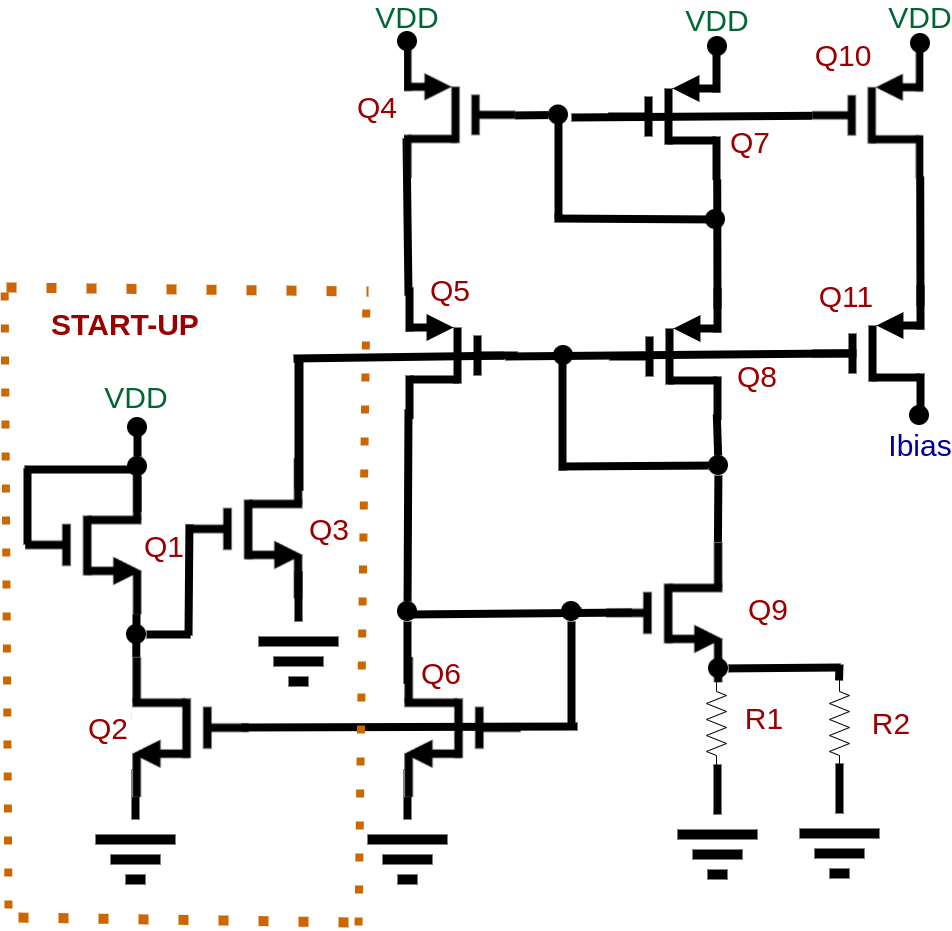
\includegraphics[scale=0.3]{Circuitos/Ibias_generator.png}
    \legend{Fonte: Produzido pelo autor}
    \label{\NomePFig}
\end{figure}

\begin{figure}[htb]
 \centering
    \centering
    \caption{Representação em bloco do \NomeBloco} \label{\NomeSFig}
    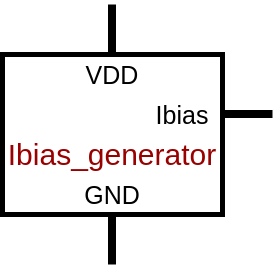
\includegraphics[scale=0.3]{Circuitos/ibias_generator_block.png}
    \legend{Fonte: Produzido pelo autor}
\end{figure}

Os transistores utilizados no bloco apresentam os par\^ametros mostrados na \autoref{\NomeTTab}.

\begin{table}[htbp]
\caption{Transistores do Bloco \NomeBloco}
\label{\NomeTTab}
\centering
\begin{tabular}{ccccc}
\toprule
Transistor & W ($\mu$m)  & L ($\mu$m)           & M (n° dispositivos) & S (n° dispositivos)\\
\midrule \midrule
Q1 & 0,3 & 19,995 & 1 & 3\\
\midrule
Q2 & 25 & 0,5 & 2 & 1\\
\midrule
Q3 & 30 & 0,5 & 1 & 1\\
\midrule
Q4, Q7 e Q10 & 35 & 4 & 2 & 1\\
\midrule
Q5, Q8 e Q11 & 25 & 2,5 & 2 & 1\\
\midrule
Q6 & 20 & 4 & 2 & 1\\
\midrule
Q9 & 20 & 4 & 4 & 1\\
\midrule
Q10 & 25 & 2,5 & 2 & 1\\
\midrule
Q11 & 25 & 2,5 & 2 & 1\\
\bottomrule
\end{tabular}
\legend{Fonte: Produzido pelo autor}
\end{table}

O resistor utilizado no bloco apresenta os par\^ametros mostrados na \autoref{\NomeQTab}.

\begin{table}[htbp]
\caption{Resistor do bloco \NomeBloco}
\label{\NomeQTab}
\centering
\begin{tabular}{ccccc}
\toprule
Resistor & W ($\mu$m)  & L ($\mu$m) & M (n° dispositivos) & Resist\^encia (k$\Omega$)\\
\midrule \midrule
R & 8 & 29,98 & 2 & 0,569025\\
\bottomrule
\end{tabular}
\legend{Fonte: Produzido pelo autor}
\end{table}

Os transistores \textit{Q6} e \textit{Q9}, juntos aos resistores \textit{R1} e \textit{R2}, t\^em a finalidade de funcionarem como um dreno de corrente referenciados pelos resistores. Os transistores \textit{Q4} e \textit{Q7} t\^em a finalidade de funcionarem como uma fonte de corrente, referenciados pelo dreno de corrente j\'a mencionado. O transistor \textit{Q10} \'e o braço do espelho de corrente do qual fornece a corrente de sa\'ida.

Os transistores \textit{Q5}, \textit{Q8} e \textit{Q11} se apresentam na configuração \textit{Cascode}, que tem o intuito de tornar o espelho de corrente de resposta mais linear, aumentar sua banda e ainda aumentar as suas resist\^encias de entrada e sa\'ida.

Os transistores \textit{Q1}, \textit{Q2} e \textit{Q3} t\^em a função de inicializar o circuito no ponto de operação adequado, j\'a que o circuito tamb\'em apresenta estabilidade quando fornecendo 0 A, sendo necess\'ario evitar essa situação.

\renewcommand{\NomeBloco}{\textit{iref\_generator}}
\renewcommand{\NomeBlocoNoUnderline}{irefgenerator}
\renewcommand{\NomePTab}{tab_\NomeBlocoNoUnderline}
\renewcommand{\NomeSTab}{tab_\NomeBlocoNoUnderline2}
\renewcommand{\NomePFig}{fig_\NomeBlocoNoUnderline}
\renewcommand{\NomeSFig}{fig_\NomeBlocoNoUnderline2}
\renewcommand{\NomeTTab}{tab_\NomeBlocoNoUnderline3}
\renewcommand{\NomeQTab}{tab_\NomeBlocoNoUnderline4}

\subsection{iref\_generator}

O bloco \NomeBloco{}\footnote{Circuito desenvolvido por \textit{Dalton Martini Colombo}, orientador do trabalho aqui apresentado} \'e um espelho de corrente que apresenta algumas sa\'idas como fonte e outras em dreno de corrente. O bloco apresenta as definições de sa\'ida referidos na \autoref{\NomeSTab}.

\begin{table}[!h]
\caption{Sinais do bloco \NomeBloco}
\label{\NomeSTab}
\centering
\begin{tabular}{ccl}

    \toprule
    Sinal & Tipo    & Descrição        \\
    \midrule \midrule
    iref1\_src   & Saída   & Fonte de Corrente de 0.5 $\mu$A \\
    \midrule
    iref2\_src   & Saída   & Fonte de Corrente de 0.5 $\mu$A \\
    \midrule
    iout\_test   & Saída   & Fonte de Corrente de 1.5 $\mu$A \\
    \midrule
    iref1\_sink   & Saída   & Dreno de Corrente de 0.5 $\mu$A \\
    \midrule
    iref2\_sink   & Saída   & Dreno de Corrente de 0.5 $\mu$A \\
    \bottomrule
\end{tabular}
\legend{Fonte: Produzido pelo autor}
\end{table}

O circuito projetado para o bloco \'e demonstrado na \autoref{\NomePFig}.

\begin{figure}[htb]
 \centering
    \centering
    \caption{Circuito CMOS projetado para o bloco \NomeBloco} 
    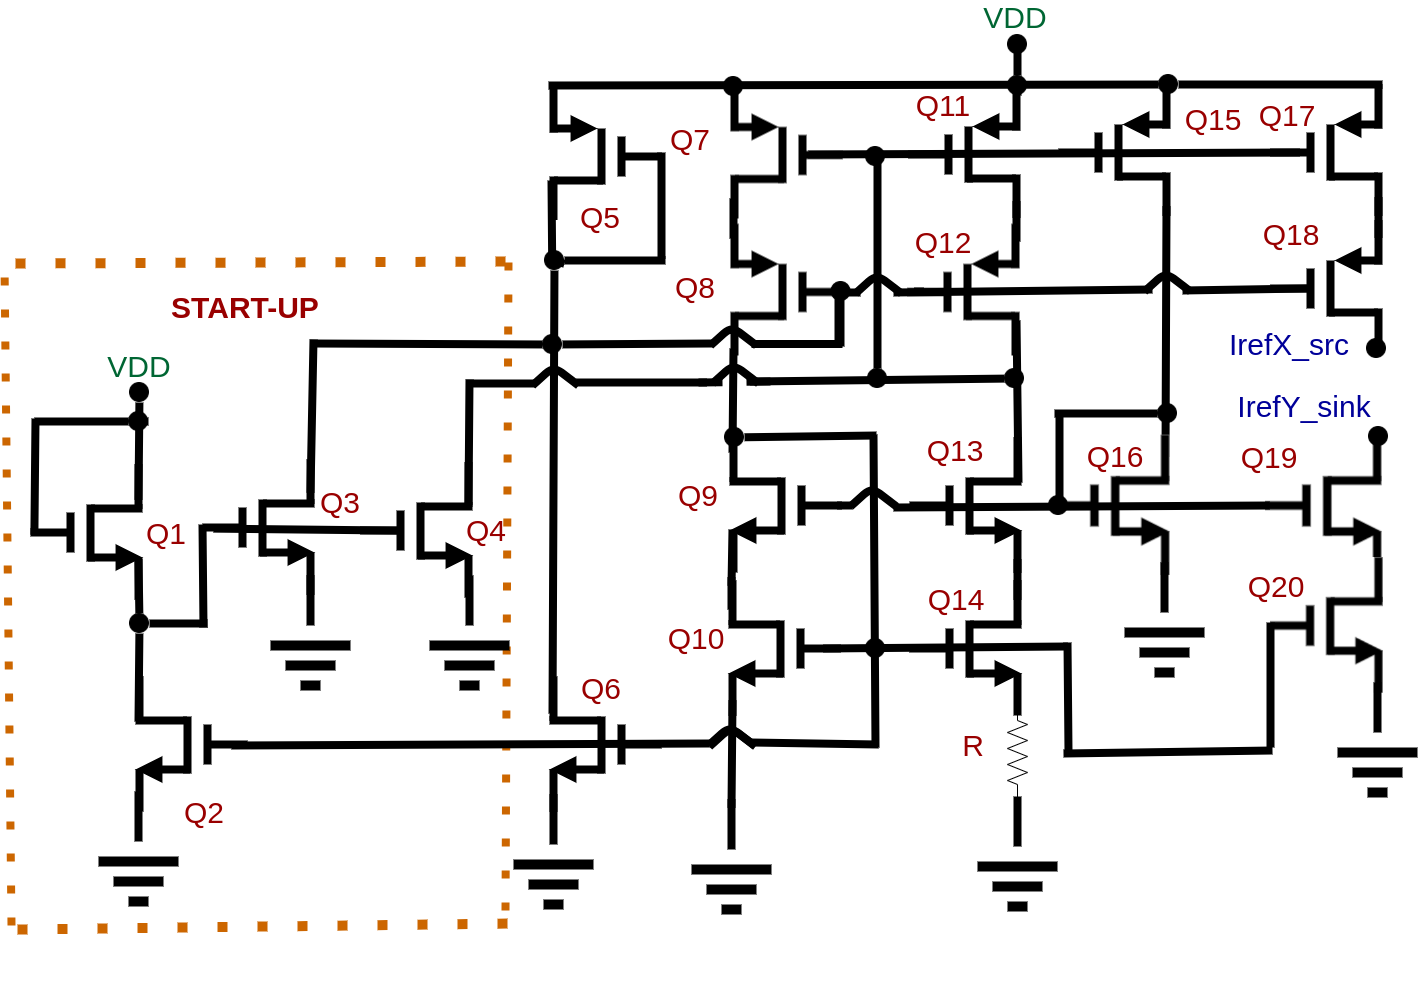
\includegraphics[scale=0.3]{Circuitos/iref_generator.png}
    \legend{Fonte: Produzido pelo autor}
    \nota{Nem todos transistores são representados na imagem. \emph{Q17}, \emph{Q18}, \emph{Q19} e \emph{Q20} são transistores replicados para cada sa\'ida \emph{IrefX\_src} e \emph{IrefY\_sink}, onde \emph{X} e \emph{Y} são os identificadores de cada sa\'ida}
    \label{\NomePFig}
\end{figure}

\begin{figure}[htb]
 \centering
    \centering
    \caption{\label{\NomeSFig}Representação em bloco do \NomeBloco}
    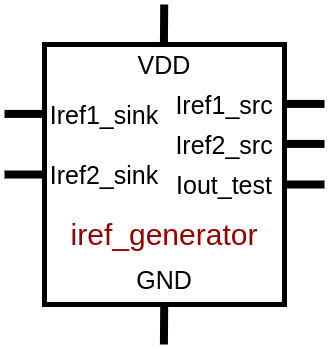
\includegraphics[scale=0.3]{Circuitos/iref_generator_block.png}
    \legend{Fonte: Produzido pelo autor}
\end{figure}

Os transistores utilizados no bloco apresentam os par\^ametros mostrados na \autoref{\NomeTTab}.

\begin{table}[!h]
\caption{Transistores do Bloco \NomeBloco}
\label{\NomeTTab}
\centering
\begin{tabular}{ccccc}
\toprule
Transistor & W ($\mu$m)  & L ($\mu$m)  & M (n° dispositivos) & S (n° dispositivos)\\
\midrule \midrule

\midrule
Q1                                   & 0,3    & 19,995 & 1                   & 3                   \\
\midrule
Q2                                   & 35     & 0,18   & 2                   & 1                   \\
\midrule
Q3 e Q4                              & 15     & 0,18   & 1                   & 1                   \\
\midrule
Q5                                   & 10     & 15     & 1                   & 6                   \\
\midrule
\begin{tabular}[c]{@{}c@{}}Q6, Q9, Q10,\\ Q13, Q19 e Q20\end{tabular}          & 4      & 19,995 & 1                   & 2                   \\
\midrule
\begin{tabular}[c]{@{}c@{}}Q7, Q8, Q11, Q12,\\ Q15, Q17a¹ e Q18a¹\end{tabular} & 10     & 15   & 2                   & 1                   \\
\midrule
Q14                                  & 4      & 19,995 & 10                  & 1                   \\
\midrule
Q16                                  & 4      & 19,995 & 1                   & 6 \\
\midrule
Q17b² e Q18b²                                                                  & 10     & 15     & 6                   & 1                  \\
\bottomrule
\end{tabular}
\legend{Fonte: Produzido pelo autor}
\legend{¹ Q17a e Q18a são os transistores referentes \`as sa\'idas iref1\_src e iref2\_src\\
² Q17b e Q18b são os transistores referentes \`a sa\'ida iout\_test}
\end{table}

O resistor \emph{R} utilizado no bloco apresenta os par\^ametros mostrado na \autoref{\NomeQTab}.

\begin{table}[!h]
\caption{Resistores do bloco \NomeBloco}
\label{\NomeQTab}
\centering
\begin{tabular}{cccc}
\toprule
Resistor & W ($\mu$m)  & L ($\mu$m) & Resist\^encia (k$\Omega$)\\
\midrule \midrule
R & 3 & 404,4 & 141,996\\
\bottomrule
\end{tabular}
\legend{Fonte: Produzido pelo autor}
\end{table}

Os transistores \emph{Q6} e \emph{Q9}, juntos aos resistores \emph{R1} e \emph{R2}, t\^em a finalidade de funcionarem como um dreno de corrente referenciados pelos resistores. Os transistores \emph{Q4} e \emph{Q7} t\^em a finalidade de funcionarem como uma fonte de corrente, referenciados pelo dreno de corrente j\'a mencionado. O transistor \emph{Q10} \'e o braço do espelho de corrente do qual fornece a corrente de sa\'ida.

Os transistores \emph{Q5}, \emph{Q8} e \emph{Q11} se apresentam na configuração \emph{Cascode}, que tem o intuito de tornar o espelho de corrente de resposta mais linear, aumentar sua banda e ainda aumentar as suas resist\^encias de entrada e sa\'ida.

Os transistores \emph{Q1}, \emph{Q2} e \emph{Q3} t\^em a função de inicializarem o circuito no ponto de operação adequado, j\'a que o circuito tamb\'em apresenta estabilidade quando fornecendo 0 A, sendo necess\'ario evitar essa situação.

\renewcommand{\NomeBloco}{current\_mirror\_nmos}
\renewcommand{\NomeBlocoNoUnderline}{curmirnmosb}
\renewcommand{\NomePTab}{tab_\NomeBlocoNoUnderline}
\renewcommand{\NomeSTab}{tab_\NomeBlocoNoUnderline2}
\renewcommand{\NomePFig}{fig_\NomeBlocoNoUnderline}
\renewcommand{\NomeSFig}{fig_\NomeBlocoNoUnderline2}
\renewcommand{\NomeTTab}{tab_\NomeBlocoNoUnderline3}
\renewcommand{\NomeQTab}{tab_\NomeBlocoNoUnderline4}

\subsubsection{\NomeBloco}

O bloco \NomeBloco{} cont\'em alguns bra{\c c}os utilizados como dreno de corrente para outras partes do circuito, sendo todos valores iguais \'a corrente de refer\^encia. O bloco apresenta as defini{\c c}\~oes de sinais de entrada e sa\'ida referidos na \autoref{\NomeSTab}.

\begin{table}[htbp]
\caption{Sinais do bloco \NomeBloco}
\label{\NomeSTab}
\centering
\begin{tabular}{ccl}

    \toprule
    Sinal & Tipo    & Descri{\c c}\~ao        \\
    \midrule \midrule
    Iref\_bias   & Entrada   &  Corrente de refer\^encia para os bra{\c c}os \\
    \midrule
    Iref\_A   & Saída   &  Bra{\c c}o 1 \\
    \midrule
    Iref\_B   & Saída   &  Bra{\c c}o 2 \\
    \midrule
    Iref\_C   & Saída   &  Bra{\c c}o 3 \\
    \midrule
    Iref\_D   & Saída   &  Bra{\c c}o 4 \\
    \midrule
    Iref\_E   & Saída   &  Bra{\c c}o 5 \\
    \bottomrule
\end{tabular}
\legend{Fonte: Produzido pelo autor}
\end{table}

O circuito projetado para o bloco \'e demonstrado na \autoref{\NomePFig}.

\begin{figure}[htb]
 \centering
    \centering
    \caption{Circuito CMOS projetado para o bloco \NomeBloco} 
    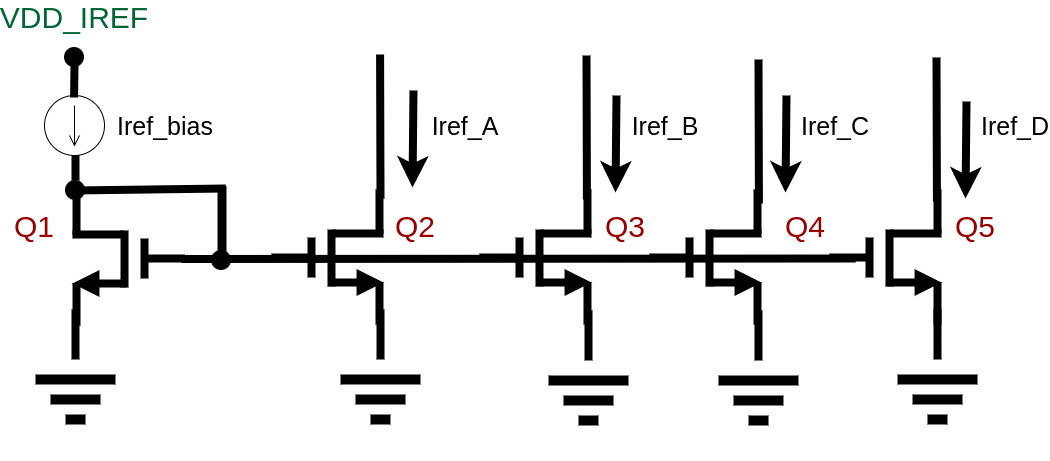
\includegraphics[scale=0.3]{Circuitos/current_mirror.png}
    \legend{Fonte: Produzido pelo autor}
    \label{\NomePFig}
\end{figure}

\begin{figure}[htb]
 \centering
    \centering
    \caption{Representa{\c c}\~ao em bloco do \NomeBloco} \label{\NomeSFig}
    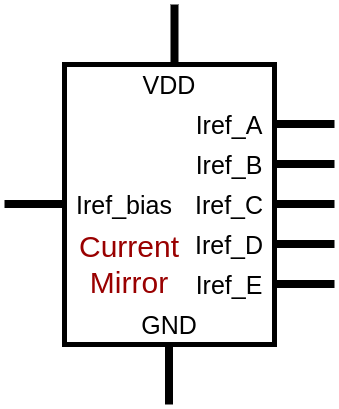
\includegraphics[scale=0.3]{Circuitos/current_mirror_block.png}
    \legend{Fonte: Produzido pelo autor}
\end{figure}

Os transistores utilizados no bloco \NomeBloco{} apresentam os par\^ametros mostrados na \autoref{\NomeTTab}.

\begin{table}[htbp]
\caption{Transistores do Bloco \NomeBloco}
\label{\NomeTTab}
\centering
\begin{tabular}{ccccc}
\toprule
Transistor & W ($\mu$m)  & L ($\mu$m)           & M (n° dispositivos) & S (n° dispositivos)\\
\midrule \midrule
\begin{tabular}[c]{@{}c@{}}Q1, Q2, Q3,\\
Q4, Q5 e Q6\end{tabular} & 5 & 6 & 2 & 1\\
\bottomrule
\end{tabular}
\legend{Fonte: Produzido pelo autor}
\end{table}

\renewcommand{\NomeBloco}{APS\_digitalized}
\renewcommand{\NomeBlocoNoUnderline}{apsdigitalized}
\renewcommand{\NomePTab}{tab_\NomeBlocoNoUnderline}
\renewcommand{\NomeSTab}{tab_\NomeBlocoNoUnderline2}
\renewcommand{\NomePFig}{fig_\NomeBlocoNoUnderline}
\renewcommand{\NomeSFig}{fig_\NomeBlocoNoUnderline2}
\renewcommand{\NomeTTab}{tab_\NomeBlocoNoUnderline3}
\renewcommand{\NomeQTab}{tab_\NomeBlocoNoUnderline4}

\section{\NomeBloco}

O \emph{APS\_digitalized} \'e o circuito respons\'avel por digitalizar o sinal gerado pelo APS descrito na \autoref{section:APS}. O bloco apresenta as defini{\c c}\~oes de sinais de entrada e sa\'ida referidos na \autoref{\NomeSTab}.

\begin{table}[htbp]
\caption{Sinais do bloco \NomeBloco}
\label{\NomeSTab}
\centering
\begin{tabular}{ccll}

    \toprule
    Sinal & Tipo    & Descri{\c c}\~ao & Observa{\c c}\~ao        \\
    \midrule \midrule
    RESET   & Entrada   & Sinal de RESET no APS & Ativo em nível baixo\\
    \midrule
    ENABLE   & Entrada   & Sinal de ENABLE no APS & Ativo em nível alto\\
    \midrule
    Vref   & Entrada   & Tens\~ao de refer\^encia utilizada pelo comparador \\
    \midrule
    Ibias   & Entrada   & Corrente de polariza{\c c}\~ao do comparador \\
    \midrule
    AnOut   & Saída   & Sinal anal\'ogico produzido pelo APS \\
    \midrule
    DigOut   & Saída   & Sinal digital produzido pelo Comparador \\
    \bottomrule
\end{tabular}
\legend{Fonte: Produzido pelo autor}
\end{table}

O circuito projetado para o bloco \'e demonstrado na \autoref{\NomePFig}.

\begin{figure}[htb]
 \label{\NomePFig}
 \centering
    \centering
    \caption{Circuito CMOS projetado para o bloco \NomeBloco} 
    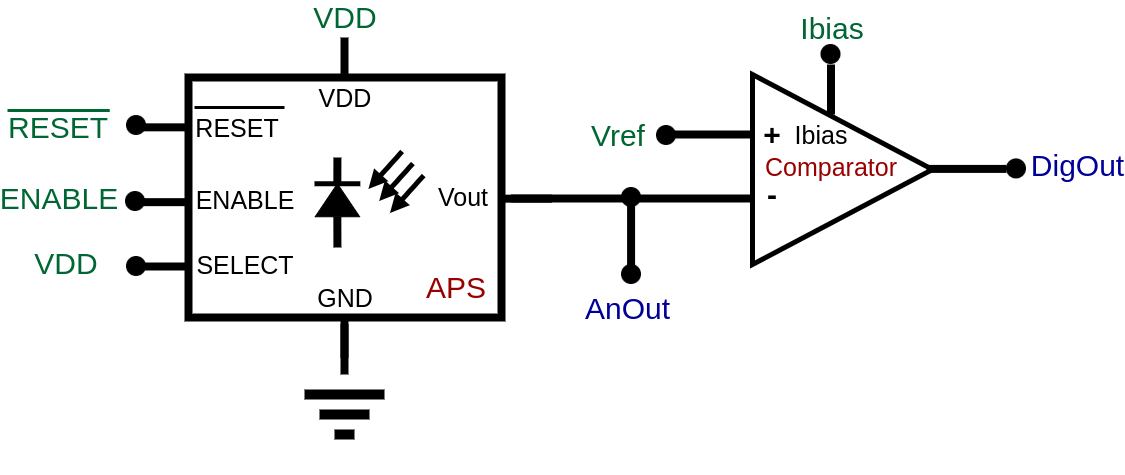
\includegraphics[scale=0.4]{Circuitos/APS_digitalized.png}
    \legend{Fonte: Produzido pelo autor}
\end{figure}

\begin{figure}[htb]
 \centering
    \centering
    \caption{Representa{\c c}\~ao em bloco do \NomeBloco} \label{\NomeSFig}
    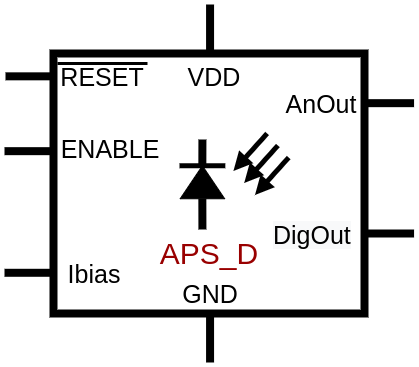
\includegraphics[scale=0.5]{Circuitos/APS_digitalized_block.png}
    \legend{Fonte: Produzido pelo autor}
\end{figure}

A sa\'ida digital do bloco funciona realizando uma compara{c c}\~ao entre uma tens\~ao de refer\^encia chamada de \emph{Vref} e a sa\'ida anal\'ogica do APS, chamada de \emph{AnOut}. Quando o valor de \emph{Vref} for maior do que o de \emph{AnOut}, o comparador ir\'a saturar e apresentar em a m\'axima tens\~ao na sa\'ida, que deve ser aproximamente igual a \emph{VDD}, interpretada como n\'ivel l\'ogico '1'. Quando o valor de \emph{Vref} for menor ou igual do que o de \emph{AnOut}, o comparador ir\'a apresentar um sinal de aproximadamente \emph{GND} em sua sa\'ida, interpretada como n\'ivel l\'ogico '0'.
Utilizando o elemento comparador, podemos ajustar para que a sa\'ida retorne '0' apenas quando for atingido um valor limiar controlado. Como sabemos que a intensidade da corrente fotogerada depende da intensidade da luz captada pelo fotodiodo (\autoref{secao_fotodiodo}), podemos deduzir a informa{\c c}\~ao sobre intensidade luminosa verificando em quanto tempo demora para que se mude de n\'ivel l\'ogico '1' para '0' durante o Est\'agio 2, utilizando-se a \autoref{eq_responsividade} e a \autoref{eq_modEletFotIl} e para se obter a \autoref{eq_apsd}.

\begin{equation}
    \label{eq_apsd}
    P = \frac{(VDD-V_{ref})(C_{j}+C_{cn})}{R_{\lambda}T}
\end{equation}

Onde:

\begin{itemize}

    \item \emph{P$_{FD}$} \'e a pot\^encia \'optica presente no fotodiodo [W]
    \item \emph{R$_\lambda$} \'e a Responsividade [A.W$^{-1}$]
    \item \emph{VDD} \'e a tens\~ao de alimenta{\c c}\~ao do circuito [$V$]
    \item \emph{$V_{ref}$} \'e a tens\~ao de refer\^encia do comparador [$V$]
    \item \emph{$C_j$} \'e a capacit\^ancia de jun{\c c}\~ao do fotodiodo [F]
    \item \emph{$C_{cn}$} \'e a capacit\^ancia do n\'o central do APS [F]
    \item $R_{\lambda}$ \'e a responsividade para o comprimento de onda detectado no fotodiodo [$A.W^{-1}$]
    \item \emph{T} \'e o per\'iodo do qual o n\'ivel l\'ogico mudou de '1' para '0' [\emph{s}]
    
\end{itemize}

Um transistor NMOS n\~ao apresentado na ilustra{\c c}\~ao foi conectado com o dreno e fonte ligados ao terra e o gate em VDD, de forma a se formar um capacitor de desacoplamento para o bloco. Os par\^ametros desse transistor s\~ao dadas na \autoref{tab_capdecapsd}.

\begin{table}[htbp]
\caption{Capacitor de desacoplamento via transistor do bloco \NomeBloco}
\label{tab_capdecapsd}
\centering
\begin{tabular}{cccc}
\toprule
W ($\mu$m)  & L ($\mu$m) & M (n° dispositivos) & S (n° dispositivos)\\
\midrule \midrule
10 & 19.995 & 1 & 1\\
\bottomrule
\end{tabular}
\legend{Fonte: Produzido pelo autor}
\end{table}
\clearpage


\renewcommand{\NomeBloco}{APS\_pixel\_clk}
\renewcommand{\NomeBlocoNoUnderline}{apspixelclk}
\renewcommand{\NomePTab}{tab_\NomeBlocoNoUnderline}
\renewcommand{\NomeSTab}{tab_\NomeBlocoNoUnderline2}
\renewcommand{\NomePFig}{fig_\NomeBlocoNoUnderline}
\renewcommand{\NomeSFig}{fig_\NomeBlocoNoUnderline2}
\renewcommand{\NomeTTab}{tab_\NomeBlocoNoUnderline3}
\renewcommand{\NomeQTab}{tab_\NomeBlocoNoUnderline4}

\section{\NomeBloco}

O \NomeBloco{} \'e o bloco respons\'avel por processar e digitalizar o sinal gerado pelo \emph{TIA}. A inten{\c c}\~ao de uso do \emph{TIA} \'e que ele seja o respons\'avel por captar um sinal luminoso com frequ\^encia bem definida, e o sinal el\'etrico gerado, em forma de pulsos quadrados, sirva de refer\^encia de rel\'ogio para todos os circuitos APS utilizados para detec{\c c}\~ao de cor. O bloco portanto tem como responsabilidade gerar um sinal digital de frequ\^encia igual \'a do sinal luminoso captado. O bloco apresenta as defini{\c c}\~oes de sinais de entrada e sa\'ida referidos na \autoref{\NomeSTab}.

\begin{table}[htbp]
\caption{Sinais do bloco \NomeBloco}
\label{\NomeSTab}
\centering
\begin{tabular}{ccl}

    \toprule
    Sinal & Tipo    & Descri{\c c}\~ao\\
    \midrule \midrule
    Vref\_comp   & Entrada   & Tens\~ao de refer\^encia utilizada pelo comparador\\
    \midrule
    Vref\_amp   & Entrada   & Tens\~ao de refer\^encia utilizada para o TIA\\
    \midrule
    Ibias   & Entrada   & Corrente de polariza{\c c}\~ao do comparador \\
    \midrule
    Vout   & Saída   & Sinal digital produzido pelo Comparador\\
    \bottomrule
\end{tabular}
\legend{Fonte: Produzido pelo autor}
\end{table}

O circuito projetado para o bloco \'e demonstrado na \autoref{\NomePFig}.

\begin{figure}[htb]
 \label{\NomePFig}
 \centering
    \centering
    \caption{Circuito CMOS projetado para o bloco \NomeBloco} 
    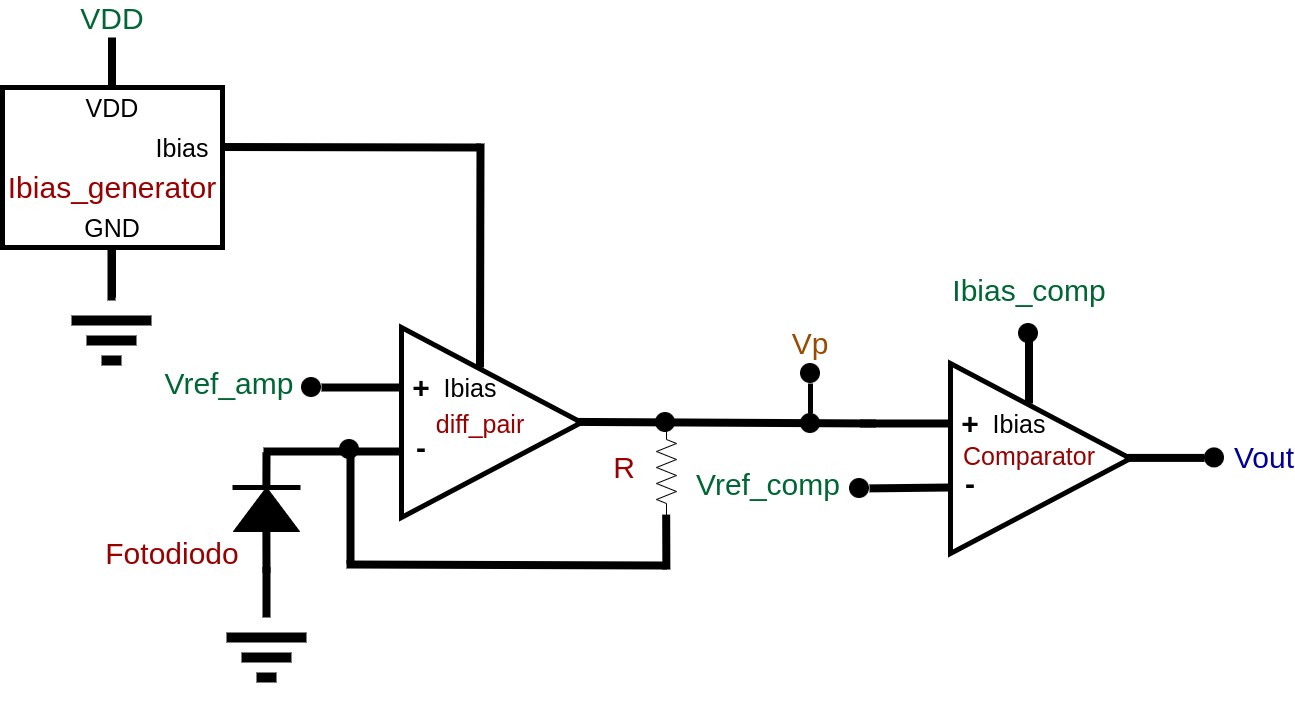
\includegraphics[scale=0.35]{Circuitos/APS_clk.png}
    \legend{Fonte: Produzido pelo autor}
\end{figure}

\begin{figure}[htb]
 \centering
    \centering
    \caption{Representa{\c c}\~ao em bloco do \NomeBloco} \label{\NomeSFig}
    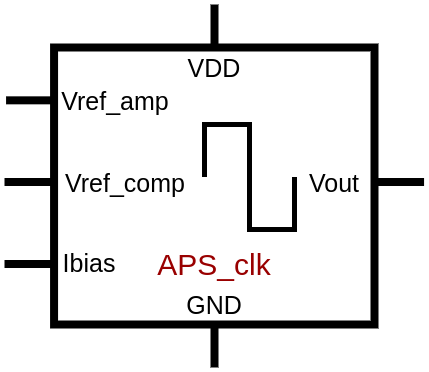
\includegraphics[scale=0.5]{Circuitos/APS_clk_block.png}
    \legend{Fonte: Produzido pelo autor}
\end{figure}

O circuito tem funcionamento similar ao do apresentado no bloco \emph{APS\_digitalized}, por\'em com apenas a sa\'ida digital sendo considerada e sendo utilizado um $TIA$ ao inv\'es de um APS. A corrente de polariza{\c c}\~ao do par diferencial \'e gerada pelo bloco Ibias\_generator presente no bloco.

Uma resist\^encia $R$ de ganho \'e utilizada, com valor apresentado na \autoref{\NomeQTab}.

\begin{table}[htb]
\caption{Resistores do bloco \NomeBloco}
\label{\NomeQTab}
\centering
\begin{tabular}{cccc}
\toprule
Resistor & W ($\mu$m)  & L ($\mu$m) & Resist\^encia (k$\Omega$)\\
\midrule \midrule
R & 1,68 & 39486,3 & 25000\\
\bottomrule
\end{tabular}
\legend{Fonte: Produzido pelo autor}
\end{table}

Para o bloco, a \autoref{eq_TIAblock} descreve $V_{PH}$, que \'e comparada com \emph{Vref\_comp} e ent\~ao utilizada para gerar o sinal de sa\'ida.

\begin{equation}
    \label{eq_TIAblock}
    V_{PH} = RI_{PH} + Vref_amp
\end{equation}

Onde:

\begin{itemize}

    \item \emph{$V_{PH}$} \'e a tens\~ao no ramo positivo do comparador [$V$]
    \item \emph{$I_{PH}$} \'e a corrente fotogerada [$A$]
    
\end{itemize}

Dois transistores NMOS n\~ao apresentados na ilustra{\c c}\~ao foram conectado com o dreno e fonte ligados ao terra e o gate em VDD, de forma a se formar um capacitor de desacoplamento para o bloco. Os par\^ametros desses transistores s\~ao dadas na \autoref{tab_capdecclk}.

\begin{table}[htbp]
\caption{Capacitores de desacoplamento via transistor do bloco \NomeBloco}
\label{tab_capdecclk}
\centering
\begin{tabular}{cccc}
\toprule
W ($\mu$m)  & L ($\mu$m) & M (n° dispositivos) & S (n° dispositivos)\\
\midrule \midrule
50 & 10 & 1 & 1\\
\bottomrule
\end{tabular}
\legend{Fonte: Produzido pelo autor}
\end{table}

Dois capacitores MOS n\~ao apresentados na ilustra{\c c}\~ao tamb\'em foram utilizados como capacitores de desacoplamento. Os par\^ametros desses capacitores s\~ao dadas na \autoref{tab_capdecclk2}.

\begin{table}[htbp]
\caption{Capacitores de desacoplamento MOS do bloco \NomeBloco}
\label{tab_capdecclk2}
\centering
\begin{tabular}{ccc}
\toprule
W ($\mu$m)  & L ($\mu$m) & Capacit\^ancia ($pF$)\\
\midrule \midrule
30 & 30 & 1,7919\\
\bottomrule
\end{tabular}
\legend{Fonte: Produzido pelo autor}
\end{table}

Dois diodos quadrados ligados reversamente em VDD e GND tamb\'em foi utilizado, com o intuito de proteger o circuito de tens\~oes reversas. Os par\^ametros desses diodos s\~ao dadas na \autoref{tab_capdecclk3}

\begin{table}[htbp]
\caption{Diodos de prote{\c c}\~ao do bloco \NomeBloco}
\label{tab_capdecclk3}
\centering
\begin{tabular}{ccc}
\toprule
W ($\mu$m)  & L ($\mu$m) & \'Area ($um^2$)\\
\midrule \midrule
3 & 3 & 9\\
\bottomrule
\end{tabular}
\legend{Fonte: Produzido pelo autor}
\end{table}
\clearpage
\renewcommand{\NomeBloco}{\textit{vref\_generator}}
\renewcommand{\NomeBlocoNoUnderline}{vrefgenerator}
\renewcommand{\NomePTab}{tab_\NomeBlocoNoUnderline}
\renewcommand{\NomeSTab}{tab_\NomeBlocoNoUnderline2}
\renewcommand{\NomePFig}{fig_\NomeBlocoNoUnderline}
\renewcommand{\NomeSFig}{fig_\NomeBlocoNoUnderline2}
\renewcommand{\NomeTTab}{tab_\NomeBlocoNoUnderline3}
\renewcommand{\NomeQTab}{tab_\NomeBlocoNoUnderline4}

\section{vref\_generator}

O \textit{\NomeBloco}\footnote{Circuito esquemático desenvolvido por \textit{Dalton Martini Colombo}} \'e o bloco respons\'avel por gerar todas as tensões de refer\^encia utilizados nos outros circuitos. O bloco apresenta as definições de sinais de entrada e sa\'ida referidos na \autoref{\NomeSTab}.

\begin{table}[htbp]
\caption{Sinais do bloco \NomeBloco}
\label{\NomeSTab}
\centering
\begin{tabular}{ccl}

    \toprule
    Sinal & Tipo    & Descrição      \\
    \midrule \midrule
    Ibias   & Entrada   & Corrente de polarização do bloco Par Diferencial \\
    \midrule
    V\_extra   & Saída   & Tensão de refer\^encia 1 \\
    \midrule
    Vref\_plus   & Saída   & Tensão de refer\^encia 2 \\
    \midrule
    Vref   & Saída   & Tensão de refer\^encia 3 \\
    \midrule
    y1   & Saída   & Tensão de refer\^encia 4 \\
    \midrule
    y2   & Saída   & Tensão de refer\^encia 5 \\
    \midrule
    y3   & Saída   & Tensão de refer\^encia 6 \\
    \midrule
    y4  & Saída   & Tensão de refer\^encia 7 \\
    \midrule
    y5   & Saída   & Tensão de refer\^encia 8 \\
    \midrule
    y6   & Saída   & Tensão de refer\^encia 9 \\
    \bottomrule
\end{tabular}
\legend{Fonte: Produzido pelo autor}
\end{table}

O circuito projetado para o bloco \'e demonstrado na \autoref{\NomePFig}.

\begin{figure}[htb]
 \label{\NomePFig}
 \centering
    \centering
    \caption{Circuito CMOS projetado para o bloco \NomeBloco} 
    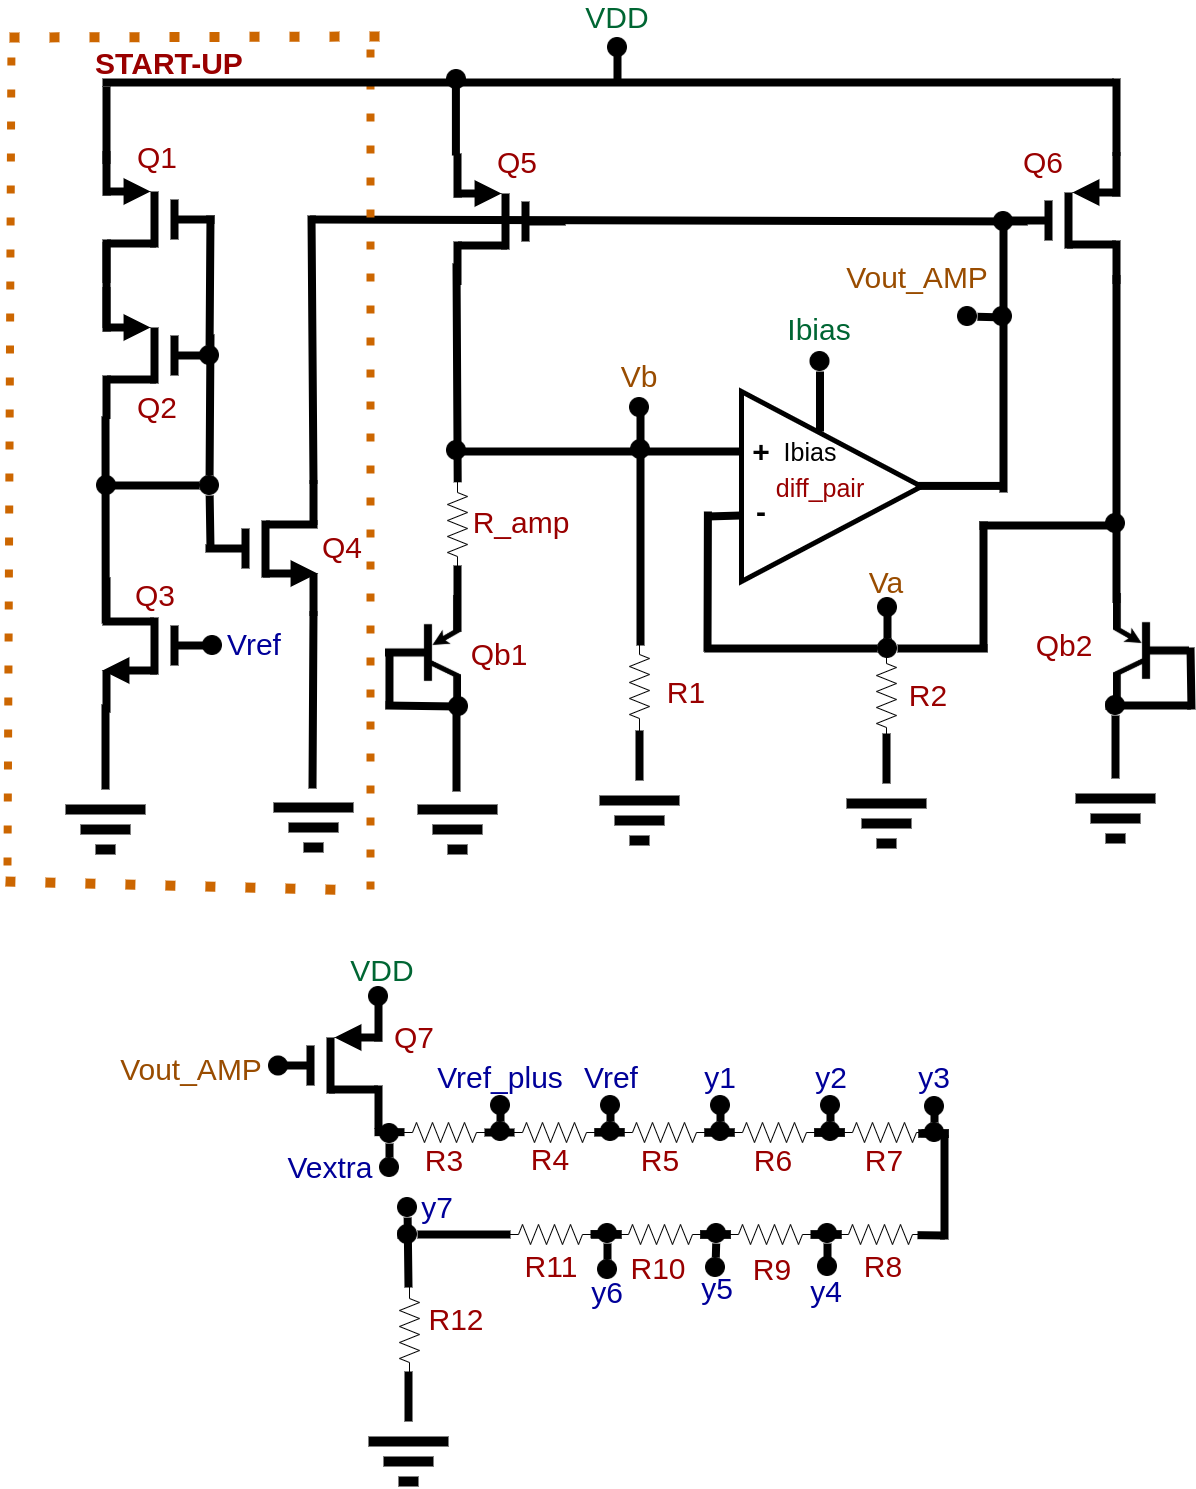
\includegraphics[scale=0.3]{Circuitos/vref_generator.png}
    \legend{Fonte: Produzido pelo autor}
\end{figure}

\begin{figure}[htb]
 \centering
    \centering
    \caption{Representação em bloco do \NomeBloco} \label{\NomeSFig}
    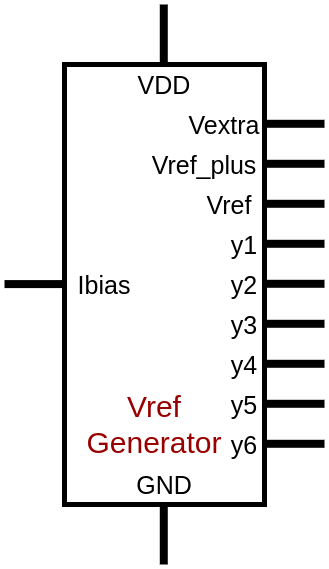
\includegraphics[scale=0.3]{Circuitos/vref_generator_block.png}
    \legend{Fonte: Produzido pelo autor}
\end{figure}

Os transistores utilizados no bloco \NomeBloco{} apresentam os par\^ametros mostrados na \autoref{\NomeTTab}.

\begin{table}[htbp]
\caption{Transistores do Bloco \NomeBloco}
\label{\NomeTTab}
\centering
\begin{tabular}{ccccc}
\toprule
Transistor & W ($\mu$m)  & L ($\mu$m)           & M (n° dispositivos) & S (n° dispositivos)\\
\midrule \midrule
Q1 e Q2 & 0,5 & 19,995 & 1 & 1\\
\midrule
Q3 & 20 & 0,18 & 1 & 1\\
\midrule
Q4 & 2 & 0,18 & 1 & 1\\
\midrule
Q5, Q6 e Q7 & 20 & 16 & 4 & 1\\
\midrule
Qb1 (PNP) & 5 & 5 & 1 & 1\\
\midrule
Qb2 (PNP) & 5 & 5 & 8 & 1\\
\bottomrule
\end{tabular}
\legend{Fonte: Produzido pelo autor}
\end{table}

Os resistores utilizados no bloco \NomeBloco{} apresentam os par\^ametros mostrados na \autoref{\NomeQTab}.

\begin{table}[htbp]
\caption{Resistores do bloco \NomeBloco}
\label{\NomeQTab}
\centering
\begin{tabular}{cccccc}
\toprule
Resistor & \begin{tabular}[c]{@{}c@{}}W \\($\mu$m)\end{tabular}   & \begin{tabular}[c]{@{}c@{}}L \\($\mu$m)\end{tabular}  & \begin{tabular}[c]{@{}c@{}}Resist\^encia\\ (k$\Omega$)\end{tabular} & \begin{tabular}[c]{@{}c@{}}M\\(n° dispositivos)\end{tabular} & \begin{tabular}[c]{@{}c@{}}S \\(n° dispositivos)\end{tabular}\\
\midrule \midrule
R1 e R2 & 2 & 18,85 & 10,1024 & 1 & 10\\
\midrule
\begin{tabular}[c]{@{}c@{}}R\_amp, R3, R4,\\ R5, R6, R7, \\ R8, R9, R10, \\ R11\end{tabular} & 2 & 18,85 & 10,1024 & 1 & 1\\
\midrule
R12 & 2 & 18,85 & 10,1024 & 7 & 1\\
\bottomrule
\end{tabular}
\legend{Fonte: Produzido pelo autor}
\end{table}

O dispositivo funciona produzindo uma corrente de refer\^encia extremamente est\'avel, utilizando um amplificador operacional e realimentação. O braço \textit{Q7} utiliza dessa corrente como refer\^encia para gerar uma corrente que alimenta alguns resistores, que geram os potenciais de refer\^encia desejados.

\renewcommand{\NomeBloco}{\emph{vref\_block}}
\newcommand{\NomeBlocoA}{vrefblock}
\renewcommand{\NomePTab}{tab_\NomeBlocoA}
\renewcommand{\NomeSTab}{tab_\NomeBlocoA2}
\renewcommand{\NomePFig}{fig_\NomeBlocoA}
\renewcommand{\NomeSFig}{fig_\NomeBlocoA2}
\renewcommand{\NomeTTab}{tab_\NomeBlocoA3}

\section{vref\_block}

O bloco \NomeBloco{} tem a finalidade de conter o bloco \emph{vref\_generator}, mais o bloco respons\'avel por gerar a corrente que o polariza. O bloco apresenta as definições de sinais de entrada e sa\'ida referidos na \autoref{\NomeSTab}.

\begin{table}[!h] 
\caption{Sinais do bloco \NomeBloco}
\label{\NomeSTab}
\centering
\begin{tabular}{ccl}

    \toprule
    Sinal & Tipo    & Descrição      \\
    \midrule \midrule
    V\_extra   & Saída   & Tensão de refer\^encia 1 \\
    \midrule
    Vref\_plus   & Saída   & Tensão de refer\^encia 2 \\
    \midrule
    Vref   & Saída   & Tensão de refer\^encia 3 \\
    \midrule
    Vref\_minus   & Saída   & Tensão de refer\^encia 4 \\
    \midrule
    Vref\_minus2   & Saída   & Tensão de refer\^encia 5 \\
    \midrule
    Vref\_minus3   & Saída   & Tensão de refer\^encia 6 \\
    \midrule
    Vref\_minus4  & Saída   & Tensão de refer\^encia 7 \\
    \midrule
    Vref\_minus5   & Saída   & Tensão de refer\^encia 8 \\
    \midrule
    Vref\_minus6   & Saída   & Tensão de refer\^encia 9 \\
    \bottomrule
\end{tabular}
\legend{Fonte: Produzido pelo autor}
\end{table}

O circuito projetado para o bloco \'e demonstrado na \autoref{\NomePFig}.

\begin{figure}[htb]
 \centering
    \centering
    \caption{\label{\NomePFig}Circuito CMOS projetado para o bloco \NomeBloco}
    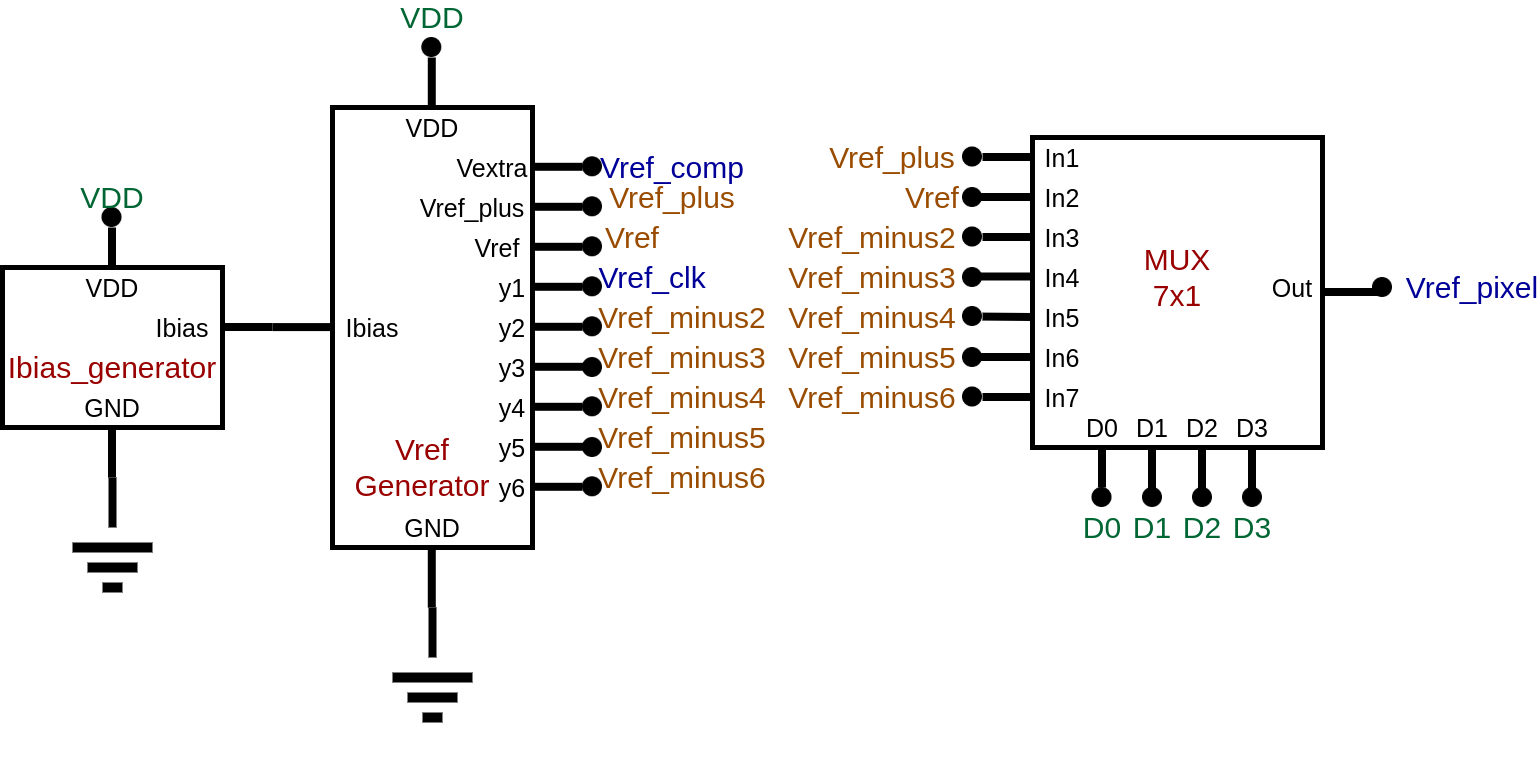
\includegraphics[scale=0.3]{Circuitos/vref_block.png}
    \legend{Fonte: Produzido pelo autor}
\end{figure}

\begin{figure}[htb]
 \centering
    \centering
    \caption{\label{\NomeSFig}Representação em bloco do \NomeBloco}
    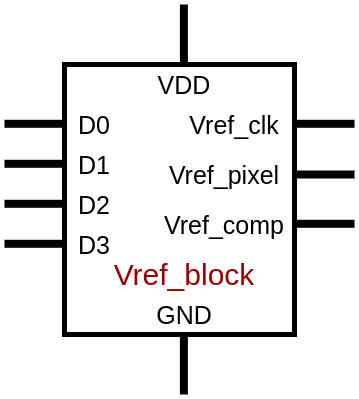
\includegraphics[scale=0.3]{Circuitos/vref_block_block.png}
    \legend{Fonte: Produzido pelo autor}
\end{figure}

\renewcommand{\NomeBloco}{\emph{vref\_block\_with\_mux}}
\renewcommand{\NomeBlocoA}{vrefblockwithmux}
\renewcommand{\NomePTab}{tab_\NomeBlocoA}
\renewcommand{\NomeSTab}{tab_\NomeBlocoA2}
\renewcommand{\NomePFig}{fig_\NomeBlocoA}
\renewcommand{\NomeSFig}{fig_\NomeBlocoA2}
\renewcommand{\NomeTTab}{tab_\NomeBlocoA3}

\section{\NomeBloco}

O bloco \NomeBloco{} tem a finalidade de selecionar a tens\~ao de refer\^encia a ser utilizada nos blocos de compara{\c c}\~ao do circuito, al\'em de retornar a tens\~ao de refer\^encia utilizada pelo bloco \emph{TIA}. A \autoref{\NomePTab} indica a Tabela Verdade do bloco. Embora tenha uma l\'ogica digital, o circuito permite sa\'idas anal\'ogicas.

\begin{table}[htbp]

\caption{Tabela Verdade do bloco \NomeBloco}%
\label{\NomePTab}
\centering
\begin{tabular}{ccccc}
    \toprule
    D0 & D1 & D2 & D3 & Out \\
    \midrule \midrule
    0 & 0 & 0 & 0 & Vref\_plus\\
    \midrule
    0 & 1 & 0 & 0 & Vref\\
    \midrule
    1 & 0 & 0 & 0 & Vref\_minus2\\
    \midrule
    1 & 1 & 0 & 0 & Vref\_minus3\\
    \midrule
    X & X & 0 & 1 & Vref\_minus4\\
    \midrule
    X & X & 1 & 0 & Vref\_minus5\\
    \midrule
    X & X & 1 & 1 & Vref\_minus6\\
\bottomrule

\end{tabular}
\fonte{Produzido pelo autor.}
\end{table}

O bloco apresenta as defini{\c c}\~oes de sinais de entrada e sa\'ida referidos na \autoref{\NomeSTab}.

\begin{table}[htbp]
\caption{Sinais do bloco \NomeBloco}
\label{\NomeSTab}
\centering
\begin{tabular}{ccl}

    \toprule
    Sinal & Tipo    & Descri{\c c}\~ao      \\
    \midrule \midrule
    D0   & Entrada   & Entrada de sele{\c c}\~ao 1 \\
    \midrule
    D1   & Entrada   & Entrada de sele{\c c}\~ao 2 \\
    \midrule
    D2   & Entrada   & Entrada de sele{\c c}\~ao 3 \\
    \midrule
    D3   & Entrada   & Entrada de sele{\c c}\~ao 4 \\
    \midrule
    Vref\_pixel   & Sa\'ida   & Tens\~ao de refer\^encia selecionada \\
    \midrule
    Vref\_clk¹  & Sa\'ida   & Tens\~ao de refer\^encia do Clock \\
    \midrule
    Vref\_comp²  & Sa\'ida   & Tens\~ao de refer\^encia do Clock do bloco teste \\
    \bottomrule
\end{tabular}
\legend{Fonte: Produzido pelo autor}
\legend{¹ Essa tens\~ao \'e igual \'a sa\'ida Vref\_minus do bloco \emph{vref\_block}\\² Essa tens\~ao \'e igual \'a sa\'ida Vref\_extra do bloco \emph{vref\_block}}
\end{table}

O circuito projetado para o bloco \'e demonstrado na \autoref{\NomePFig}.

\begin{figure}[htb]
 \label{NomePFig}
 \centering
    \centering
    \caption{Circuito CMOS projetado para o bloco \NomeBloco} \label{\NomePFig}
    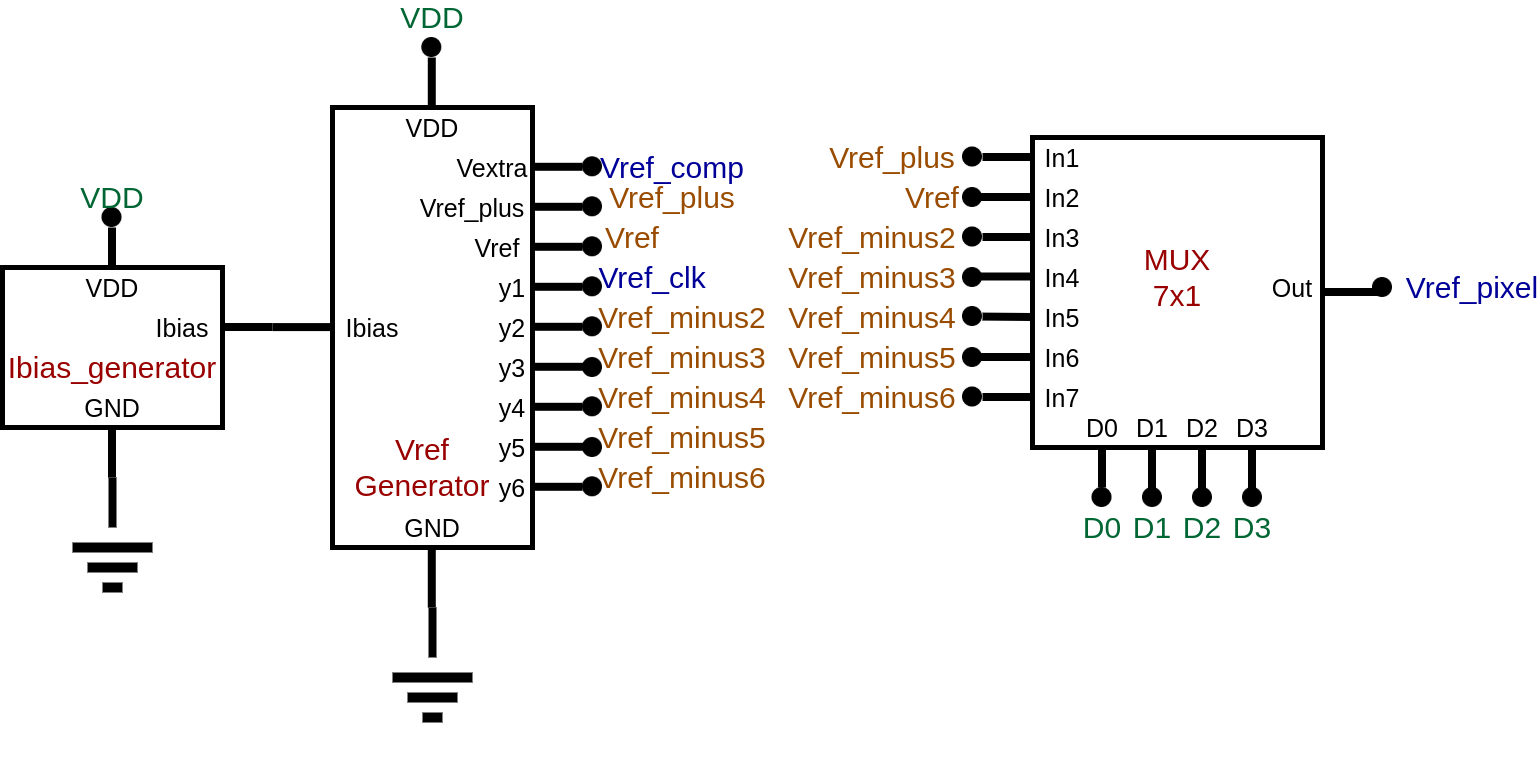
\includegraphics[scale=0.28]{Circuitos/vref_block.png}
    \legend{Fonte: Produzido pelo autor}
\end{figure}

\begin{figure}[htb]
 \label{NomeSFig}
 \centering
    \centering
    \caption{Representa{\c c}\~ao em bloco do \NomeBloco} \label{NomeSFig}
    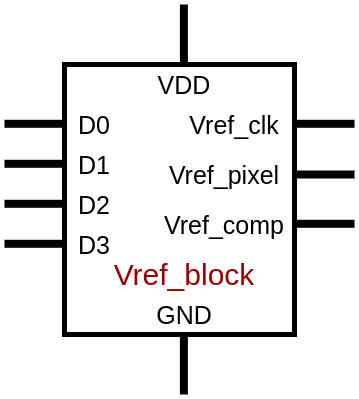
\includegraphics[scale=0.3]{Circuitos/vref_block_block.png}
    \legend{Fonte: Produzido pelo autor}
\end{figure}

\renewcommand{\NomeBloco}{ibias\_block}
\renewcommand{\NomeBlocoA}{ibiasblock}
\renewcommand{\NomePTab}{tab_\NomeBlocoA}
\renewcommand{\NomeSTab}{tab_\NomeBlocoA2}
\renewcommand{\NomePFig}{fig_\NomeBlocoA}
\renewcommand{\NomeSFig}{fig_\NomeBlocoA2}
\renewcommand{\NomeTTab}{tab_\NomeBlocoA3}

O bloco \NomeBloco{} gera diversos drenos de corrente utilizadas por outros blocos. O bloco apresenta as defini{\c c}\~oes de sinais de entrada e sa\'ida referidos na \autoref{\NomeSTab}.

\begin{table}[htbp]
\caption{Sinais do bloco \NomeBloco}
\label{\NomeSTab}
\centering
\begin{tabular}{ccl}

    \toprule
    Sinal & Tipo    & Descri{\c c}\~ao      \\
    \midrule \midrule
    bias\_pixel\_1   & Sa\'ida   & Dreno de corrente para o APS 1 (0,5 $\mu$A) \\
    \midrule
    bias\_pixel\_2   & Sa\'ida   & Dreno de corrente para o APS 2 (0,5 $\mu$A) \\
    \midrule
    bias\_pixel\_3   & Sa\'ida   & Dreno de corrente para o APS 3 (0,5 $\mu$A) \\
    \midrule
    bias\_pixel\_4   & Sa\'ida   & Dreno de corrente para o APS 4 (0,5 $\mu$A) \ \\
    extra\_500nA   & Sa\'ida   & Dreno de corrente para o APS de teste (0,5 $\mu$A) \ \\
    \midrule
    bias\_comp\_1   & Sa\'ida   & Dreno de corrente para o Comparador 1 (1,5 $\mu$A) \ \\
    \midrule
    bias\_comp\_2   & Sa\'ida   & Dreno de corrente para o Comparador 2 (1,5 $\mu$A) \ \\
    \midrule
    bias\_comp\_3   & Sa\'ida   & Dreno de corrente para o Comparador 3 (1,5 $\mu$A) \\
    \midrule
    bias\_comp\_4   & Sa\'ida   & Dreno de corrente para o Comparador 4 (1,5 $\mu$A) \\
    extra\_1500nA   & Sa\'ida   & Dreno de corrente para o Comparador de teste (1,5 $\mu$A) \ \\
    \bottomrule
\end{tabular}
\legend{Fonte: Produzido pelo autor}
\legend{¹ Essa tens\~ao \'e igual \'a sa\'ida Vref\_minus do bloco \emph{vref\_block}\\² Essa tens\~ao \'e igual \'a sa\'ida Vref\_extra do bloco \emph{vref\_block}}
\end{table}

O circuito projetado para o bloco \'e demonstrado na \autoref{\NomePFig}.

\begin{figure}[htb]
 \label{NomePFig}
 \centering
    \centering
    \caption{Circuito CMOS projetado para o bloco \NomeBloco} \label{\NomePFig}
    \includegraphics[scale=0.38]{Circuitos/ibias_block.png}
    \legend{Fonte: Produzido pelo autor}
\end{figure}

\begin{figure}[htb]
 \label{NomeSFig}
 \centering
    \centering
    \caption{Representa{\c c}\~ao em bloco do \NomeBloco} \label{NomeSFig}
    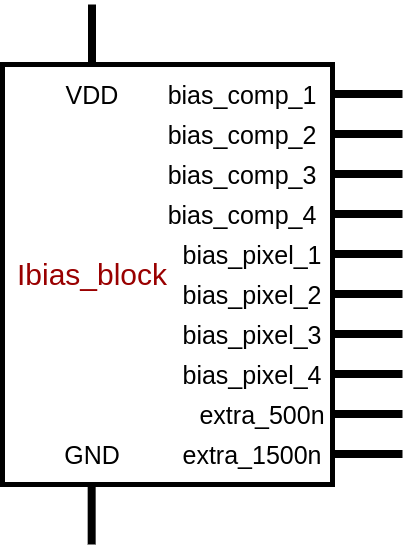
\includegraphics[scale=0.3]{Circuitos/ibias_block_block.png}
    \legend{Fonte: Produzido pelo autor}
\end{figure}
\clearpage
\renewcommand{\NomeBloco}{\textit{APS\_3}}
\renewcommand{\NomeBlocoNoUnderline}{apsthree}
\renewcommand{\NomePTab}{tab_\NomeBlocoNoUnderline}
\renewcommand{\NomeSTab}{tab_\NomeBlocoNoUnderline2}
\renewcommand{\NomePFig}{fig_\NomeBlocoNoUnderline}
\renewcommand{\NomeSFig}{fig_\NomeBlocoNoUnderline2}
\renewcommand{\NomeTTab}{tab_\NomeBlocoNoUnderline3}
\renewcommand{\NomeQTab}{tab_\NomeBlocoNoUnderline4}

\section{APS\_3}

O \textit{\NomeBloco} \'e o circuito respons\'avel por armazenar todos os tr\^es blocos APS de cor (Azul, Verde, Vermelho), mais o TIA geradora de rel\'ogio de refer\^encia para os APS's citados. O bloco apresenta as definicões de sa\'ida referidos na \autoref{\NomeSTab}.

\begin{figure}[!h]
 \centering
    \centering
    \caption{\label{\NomeSFig}Representacão em bloco do \NomeBloco}
    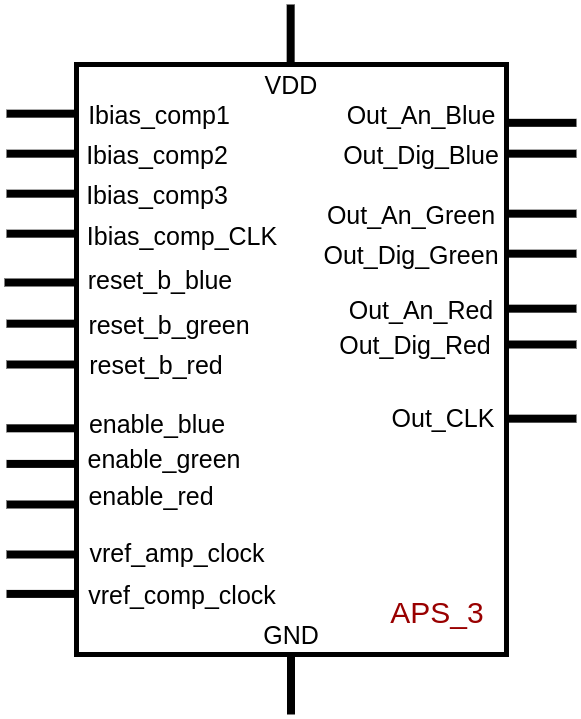
\includegraphics[scale=0.3]{Circuitos/APS_3_block.png}
    \legend{Fonte: Produzido pelo autor}
\end{figure}

\begin{table}[!h]
\centering
  \caption{Descricão dos sinais de entrada e sa\'ida do circuito projetado para as cores azul, verde e vermelha}%
  \label{\NomeSTab}
  \begin{tabular}{ccll}
  \toprule
   Sinal & Tipo & Descricão & Observacão \\
  \midrule \midrule
   RESET\_BLUE & Entrada & \begin{tabular}[l]{@{}l@{}}Sinal de tensão \textit{RESET}\\ no APS para cor azul\end{tabular} & Ativo em n\'ivel baixo \\
  \midrule
   RESET\_GREEN & Entrada & \begin{tabular}[l]{@{}l@{}}Sinal de tensão de \textit{RESET}\\ no APS para cor verde\end{tabular} & Ativo em n\'ivel baixo \\
  \midrule
   RESET\_RED & Entrada & \begin{tabular}[l]{@{}l@{}}Sinal de tensão \textit{RESET}\\ no APS para cor vermelha\end{tabular} & Ativo em n\'ivel baixo \\
   \midrule
   ENABLE\_BLUE & Entrada & \begin{tabular}[l]{@{}l@{}}Sinal de tensão \textit{ENABLE} \\no APS para cor azul\end{tabular} & Ativo em n\'ivel alto \\
  \midrule
   ENABLE\_GREEN & Entrada & \begin{tabular}[l]{@{}l@{}}Sinal de tensão \textit{ENABLE} \\no APS para cor verde\end{tabular} & Ativo em n\'ivel alto \\
  \midrule
   ENABLE\_RED & Entrada & \begin{tabular}[l]{@{}l@{}}Sinal de tensão \textit{ENABLE}\\ no APS para cor vermelha\end{tabular} & Ativo em n\'ivel alto \\
  \midrule
   Ibias\_comp1 & Entrada & \begin{tabular}[l]{@{}l@{}}Fonte de corrente para\\ cor Azul\end{tabular} &  \\
   \midrule
   Ibias\_comp2 & Entrada & \begin{tabular}[l]{@{}l@{}}Fonte de corrente para\\ cor Verde\end{tabular} &  \\
   \midrule
   Ibias\_comp3 & Entrada & \begin{tabular}[l]{@{}l@{}}Fonte de corrente para\\ cor Vermelha\end{tabular} &  \\
   \midrule
   Ibias\_clk & Entrada & \begin{tabular}[l]{@{}l@{}}Fonte de corrente para o\\ bloco \textit{APS\_pixel\_clk}\end{tabular}
    &  \\
  \midrule
   Out\_An\_Blue & Sa\'ida & \begin{tabular}[l]{@{}l@{}}Sinal anal\'ogico para cor\\ azul\end{tabular} \\
  \midrule
   Out\_Dig\_Blue & Sa\'ida & Sinal digital para cor azul \\
  \midrule
   Out\_An\_Green & Sa\'ida & \begin{tabular}[l]{@{}l@{}}Sinal anal\'ogico para cor\\ verde\end{tabular} \\
  \midrule
   Out\_Dig\_Green & Sa\'ida & Sinal digital para cor verde \\
  \midrule
   Out\_An\_Red & Sa\'ida & \begin{tabular}[l]{@{}l@{}}Sinal anal\'ogico para cor\\ vermelha\end{tabular} \\
  \midrule
   Out\_Dig\_Red & Sa\'ida & \begin{tabular}[l]{@{}l@{}}Sinal digital para cor\\ vermelha\end{tabular} \\
  \bottomrule
  \end{tabular}
  \legend{Fonte: Produzido pelo autor.}
\end{table}

O circuito projetado para o bloco \'e demonstrado na \autoref{\NomePFig}.

\clearpage

\begin{figure}[!h]
 \centering
    \centering
    \caption{Circuito CMOS projetado para o bloco \NomeBloco} 
    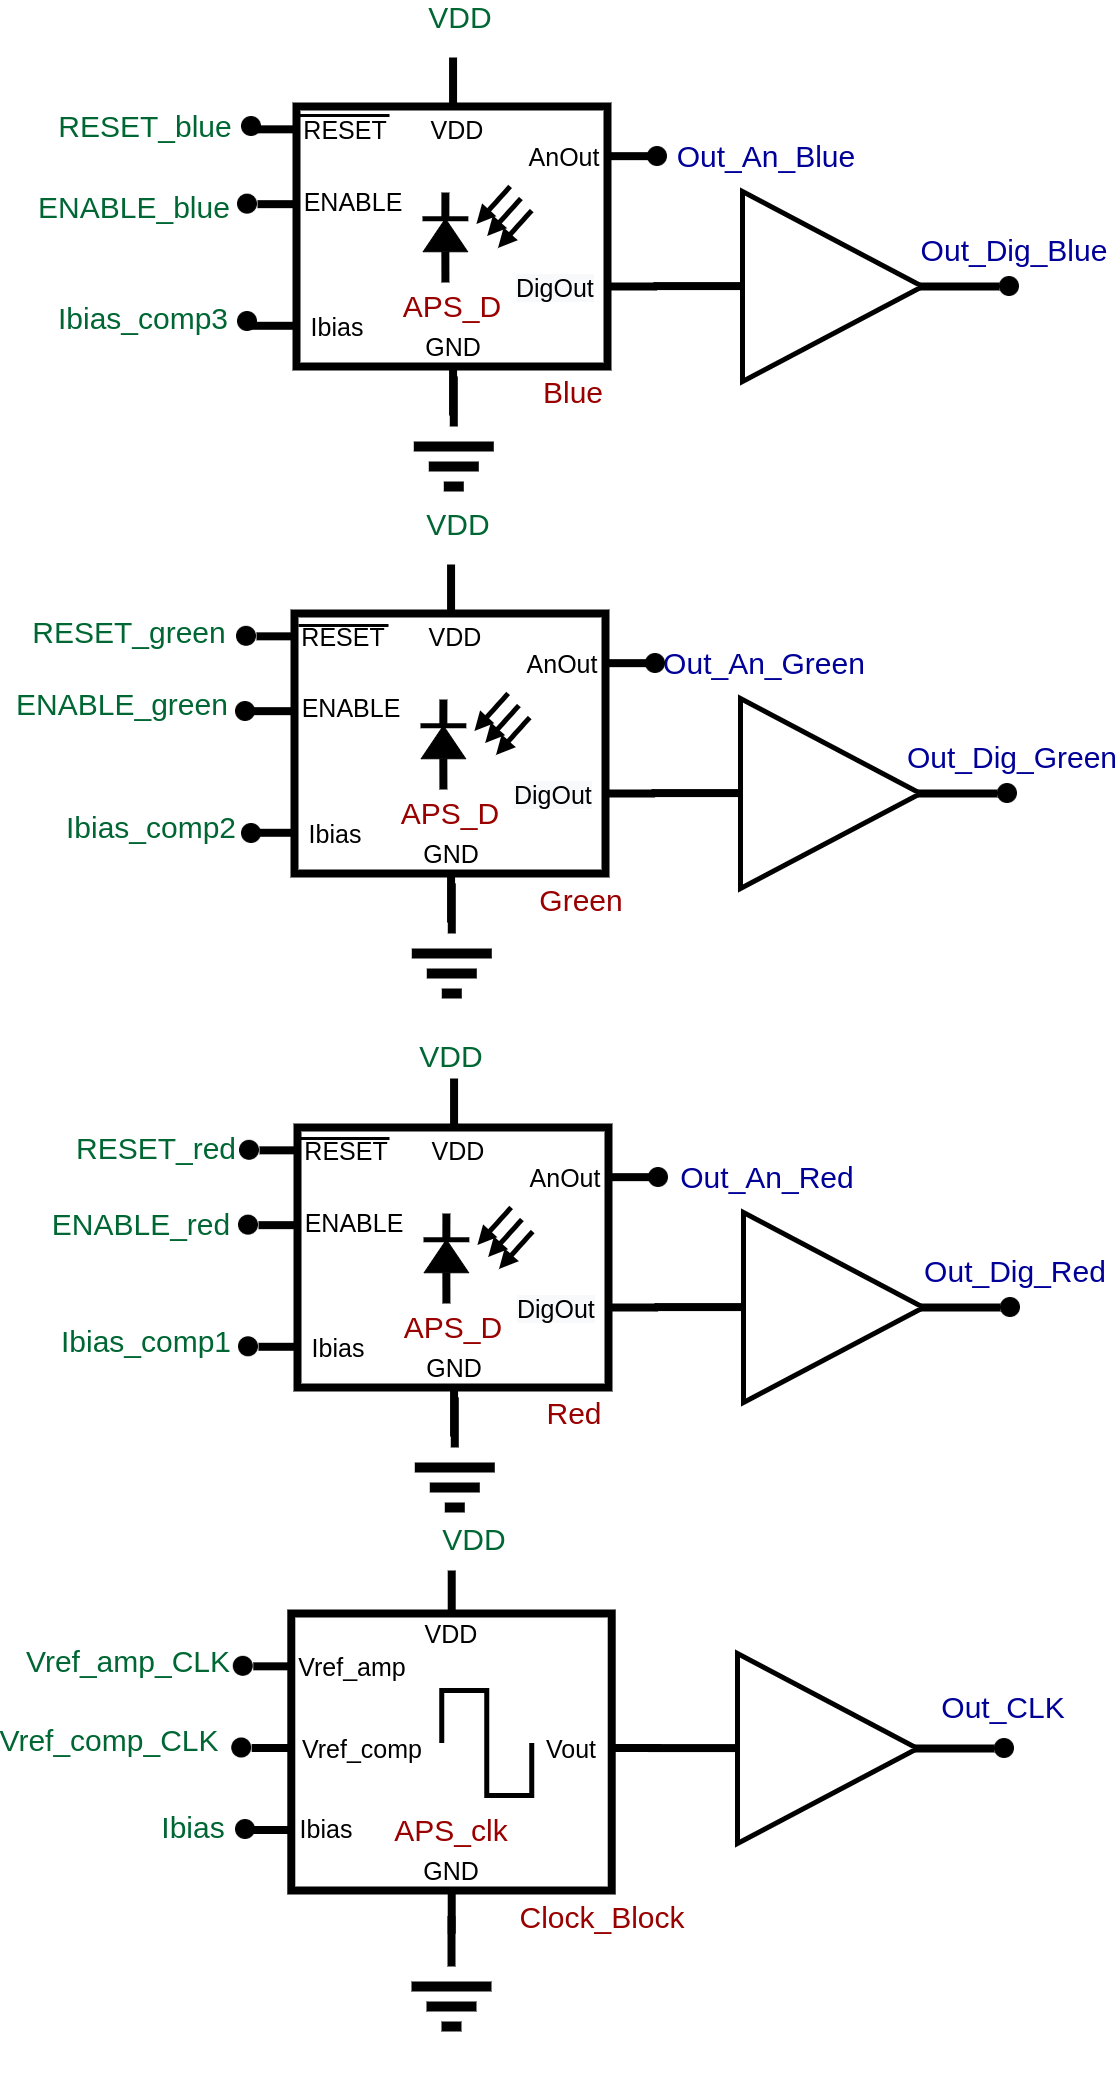
\includegraphics[scale=0.3]{Circuitos/APS_3.png}
    \legend{Fonte: Produzido pelo autor}
    \label{\NomePFig}
\end{figure}

As sa\'idas digitais de cada bloco APS\_digitalized apresentam um buffer, de forma a garantir a integridade do sinal nos pinos do Circuito Integrado.
\renewcommand{\NomeBloco}{\emph{Comparador}}
\renewcommand{\NomeBlocoNoIt}{Comparador}
\renewcommand{\NomePTab}{tab_\NomeBloco}
\renewcommand{\NomeSTab}{tab_\NomeBlocoNoIt2}
\renewcommand{\NomePFig}{fig_\NomeBlocoNoIt}
\renewcommand{\NomeSFig}{fig_\NomeBlocoNoIt2}
\renewcommand{\NomeTTab}{tab_\NomeBlocoNoIt3}

\section{\NomeBloco}

O bloco \NomeBloco{} tem a fun{\c c}\~ao de comparar dois sinais anal\'ogicos advindos nas entradas '+' (\emph{Vp}) e '-' (\emph{Vn}), e retornar \emph{VDD} caso Vp seja maior do que Vn, e \emph{GND} caso Vp seja menor ou igual a Vn.  O bloco apresenta as defini{\c c}\~oes de sinais de entrada e sa\'ida referidos na \autoref{\NomeSTab}.

\begin{table}[htbp]
\caption{Sinais do bloco \NomeBloco}
\label{\NomeSTab}
\centering
\begin{tabular}{ccl}

    \toprule
    Sinal & Tipo    & Descri{\c c}\~ao        \\
    \midrule \midrule
    Vp (+) & Entrada & Entrada positiva do Comparador\\
    \midrule
    Vn (-) & Entrada & Entrada negativa do Comparador\\
    \midrule
    Ibias & Entrada & Corrente de polariza{\c c}\~ao do Comparador\\
    \midrule
    Vo & sa\'ida & Sa\'ida do Comparador\\
    \bottomrule
\end{tabular}
\legend{Fonte: Produzido pelo autor}
\end{table}

O circuito projetado para o bloco \'e demonstrado na \autoref{\NomePFig}.

\begin{figure}[htb]
 \label{\NomePFig}
 \centering
    \centering
    \caption{Circuito CMOS projetado para o bloco \NomeBloco} 
    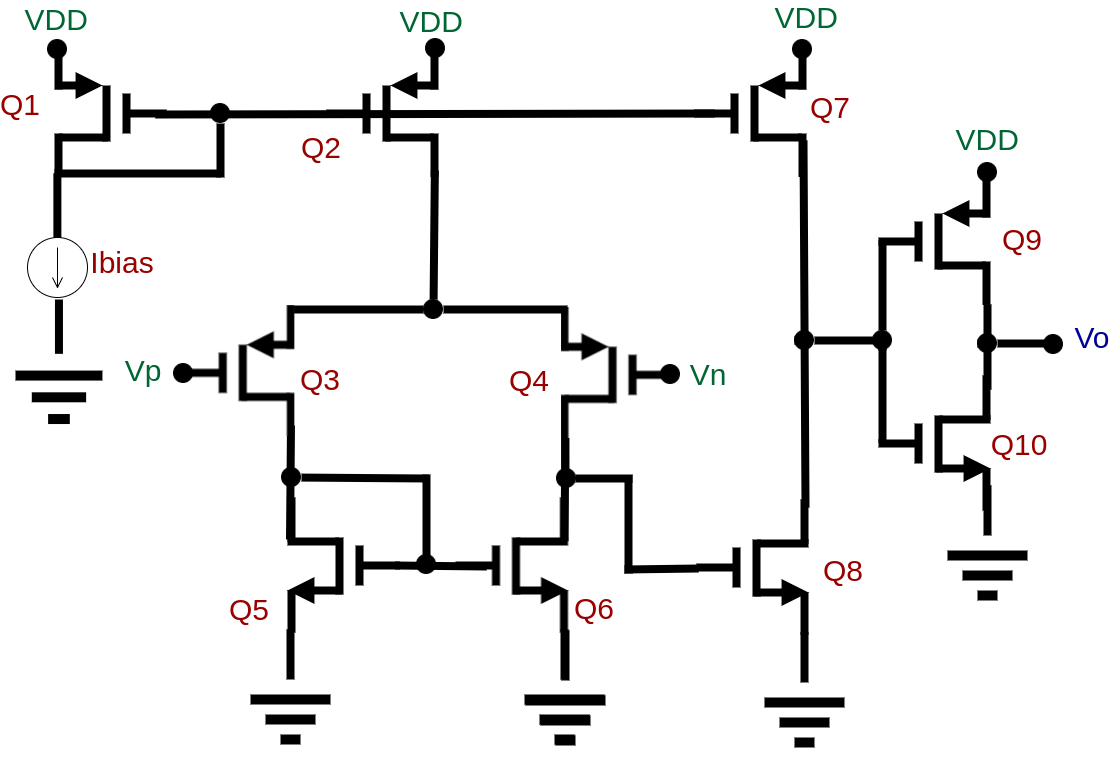
\includegraphics[scale=0.3]{Circuitos/Comparator.png}
    \legend{Fonte: Produzido pelo autor}
\end{figure}

\begin{figure}[htb]
 \centering
    \centering
    \caption{Representa{\c c}\~ao em bloco do \NomeBloco} \label{\NomeSFig}
    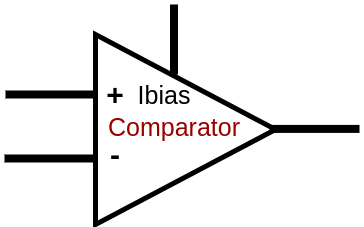
\includegraphics[scale=0.3]{Circuitos/Comparator_block.png}
    \legend{Fonte: Produzido pelo autor}
\end{figure}

Os transistores utilizados no bloco \NomeBloco{} apresentam os par\^ametros mostrados na \autoref{\NomeTTab}.

\begin{table}[htbp]
\caption{Transistores do Bloco \NomeBloco}
\label{\NomeTTab}
\centering
\begin{tabular}{ccccc}
\toprule
Transistor & W ($\mu$m)  & L ($\mu$m)           & M (n° dispositivos) & S (n° dispositivos)\\
\midrule \midrule
Q1 & 10 & 1 & 1 & 1\\
\midrule
Q2$^1$ & 10 & 1 & 6 & 6\\
\midrule
Q3 & 4 & 1 & 2 & 2\\
\midrule
Q4 & 4 & 1 & 2 & 2\\
\midrule
Q5 & 2 & 1 & 2 & 2\\
\midrule
Q6 & 2 & 1 & 2 & 2\\
\midrule
Q7$^1$ & 10 & 1 & 8 & 8\\
\midrule
Q8 & 2 & 1 & 4 & 4\\
\midrule
Q9 & 3 & 0.18 & 1 & 1\\
\midrule
Q10 & 1.5 & 0.18 & 1 & 1\\

\bottomrule
\end{tabular}
\legend{Fonte: Produzido pelo autor}
\legend{$^1$Calculado de forma a produzir uma corrente de 9 $\mu$A}
\end{table}
 
O \NomeBloco{} \'e desenvolvido com tr\^es est\'agios de amplifica{\c c}\~ao. O primeiro est\'agio, composto pelos transistores Q3, Q4, Q5, Q6 t\^em a fun{\c c}\~a de realizar a diferen{\c c}a entra as entradas \emph{Vp} e \emph{Vn} e multiplicar por um pequeno ganho. Os transistores Q3 e Q4 sao respons\'aveis por receber as entradas, enquanto os transistores Q5 e Q6 funcionam como transistores de Carga Ativa. O Q2 funciona como uma fonte de corrente.

O segundo est\'agio \'e um est\'agio de ganho, do qual o transistor Q2 fornece um ganho para a saida do est\'agio anterior e o transistor Q7 funciona como uma fonte de corrente para o est\'agio.

Diodos quadrados \emph{D1} e \emph{D2} de prote{\c c}\~ao s\~ao inclu\'idos nos terminais \emph{Vp} e \emph{Vn do circuito}, com \^anodo ligado ao terra e catodo ligado ao seu respectivo terminal. Os diodo apresentam os seguintes par\^ametros apresentados na \autoref{diodosComp}.

\begin{table}[htbp]
\caption{Diodos do Bloco \NomeBloco}
\label{diodosComp}
\centering
\begin{tabular}{cccc}
\toprule
Diodo & W ($\mu$m)  & L ($\mu$m)           & \'Area ($\mu$m²)\\
\midrule \midrule
D1 e D2 & 1 & 1 & 1 \\

\bottomrule
\end{tabular}
\legend{Fonte: Produzido pelo autor}
\end{table}

\section{Circuitos de Teste}
\label{BlocoTestes}

O circuito apresenta dois circuitos de teste adicionais, sendo um para um APS e outro para o TIA. A finalidade destes circuitos \'e de testar o sistema sem a necessidade de uma fonte luminosa. Para isso \'e acrescentado um pino diretamente aos catodos dos fotodiodos, em que uma tensão pode ser diretamente injetada nos mesmos de forma a simular a fotogeração.

O APS de teste utiliza os pinos de RESET e ENABLE iguais ao do APS de cor azul, mas \'e polarizado com uma fonte de corrente pr\'opria e também apresenda sa\'idas pr\'oprias. Caso se mantenha o pino de injeção de corrente flutuante, o APS deve funcionar de forma equivalente aos outros.
\chapter{Resultados}
\section{Simulações}

Simulações foram realizadas para testar os dispositivos projetados. Os testes avaliaram o funcionamento geral do circuito de acordo com as especificações do projeto, e também o funcionamento dos componentes APS e TIA.

Para a realização das simulações, é necessário se realizar uma estimativa da fotocorrente gerada dos fotodiodos. Como até o momento da simulação não havia a disponibilidade de uma amostra do fotodiodo utilizado, o autor fez uma estimativa conforme o trabalho de \cite{LidianeCampos}, apresentado na \autoref{tab_estcur}.

\begin{table}[htbp]
\caption{Estimativa de faixa de fotocorrente gerada}
\label{tab_estcur}
\centering
\begin{tabular}{cc}
\toprule
& Corrente nA \\
\midrule \midrule
Mínimo & 0,1\\
\midrule
Maximo & 30\\
\bottomrule
\end{tabular}
\legend{Fonte: Produzido pelo autor baseado no trabalho \cite{LidianeCampos}}
\end{table}

\subsection{Máximo sinal DC do APS}
\label{DCAPS}

É avaliado qual é o sinal DC que o bloco APS apresenta sem ter nenhuma fotocorrente gerada, $T_{enable}$ desabilitado e $T_{reset}$ habilitado. Na situação $V_{cn}$ irá apresentar o valor de VDD, o que vai representar o máximo sinal possível em $V_{out}$. A corrente \textit{Iref} considerada foi de $500$ nA, fornecida pelo bloco \textit{current\_mirror\_nmos}. Uma carga de $100$ fF foi utilizada na saída do APS de forma a simular a conexão com  um transistor na saída. O valor obtido foi de $1,15813$ V para $V_{out}$.

\subsection{Máximo sinal DC do APS no APS\_digitalized}

É avaliado qual é o sinal DC que o bloco APS conectado a um comparador apresenta sem ter nenhuma fotocorrente gerada, $T_{enable}$ desabilitado e $T_{reset}$ habilitado. Na situação $V_{cn}$ irá apresentar o valor de VDD, o que vai representar o máximo sinal possível em $V_{out}$. A corrente \textit{Iref} utilizada para a simulação foi de $500$ nA, fornecida pelo bloco \textit{current\_mirror\_nmos}. Uma carga de $100$ fF foi utilizada na saída do APS de forma a simular outras capacitâncias que podem aparecer no nó. O valor obtido foi de $1,15813$ V para $V_{out}$, equivalente ao apresentado na \autoref{DCAPS}.

\subsection{Máximo sinal DC do APS no APS\_digitalized}

É avaliado qual é o sinal DC que o bloco APS conectado a um comparador apresenta sem ter nenhuma fotocorrente gerada, $T_{enable}$ desabilitado e $T_{reset}$ habilitado. Na situação $V_{cn}$ irá apresentar o valor de VDD, o que vai representar o máximo sinal possível em $V_{out}$. A corrente \textit{Iref} utilizada para a simulação foi de $500$ nA, fornecida pelo bloco \textit{current\_mirror\_nmos}. Uma carga de $100$ fF foi utilizada na saída do APS de forma a simular outras capacitâncias que podem aparecer no nó. O valor obtido foi de $1,15813$ V para $V_{out}$, equivalente ao apresentado na \autoref{DCAPS}.

\subsection{Análise transiente do sinal de saída}

É avaliado qual a resposta do APS com a presença de uma fotocorrente. Para a simulação, foi considerado o modelo apresentado na \autoref{fig_APS_cap}, do qual há uma fonte de corrente em paralelo a um diodo representando a fotogeração. A corrente \textit{Iref} considerada foi de $500$ nA, fornecida pelo bloco \textit{current\_mirror\_nmos}.

O Período de Reset é sempre definido para ter uma duração de $1$ us, de forma que esse valor precisa ser suficiente para que o sinal em $V_{cn}$ estabilize em VDD (como discutido na \autoref{secao_amostrando}). Dois valores para o Período de Integração foram considerados, como mostrado nas próximas subseções.

\subsection{Período de Integração igual a 121 $\mu$s}

Nessa situação, foi considerado uma fotocorrente de 5 nA, que está dentro da faixa proposta pelo autor na \autoref{tab_estcur}. Os resultados obtidos são observados nos gráficos abaixo.

\begin{figure}[htb]
 \centering
  \begin{minipage}{0.4\textwidth}
    \centering
    \caption{   A}
    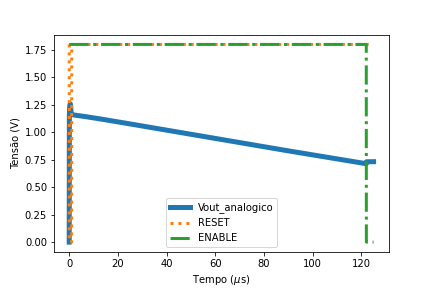
\includegraphics[scale=0.8]{Resultados/Graficos/reseteenable-tb_pixel125.png}
    \legend{Fonte: Produzido pelo autor}
  \end{minipage}
  \hfill
  \begin{minipage}{0.4\textwidth}
    \centering
    \caption{A} 
    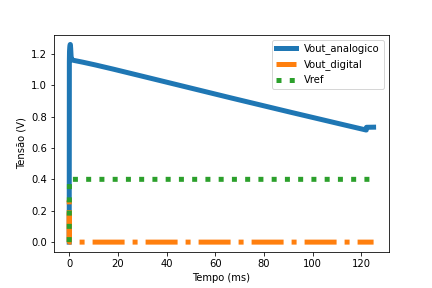
\includegraphics[scale=0.8]{Resultados/Graficos/analogicoedigital-tb_pixel125.png}
    \legend{Fonte: Produzido pelo autor}
  \end{minipage}
\end{figure}

\subsection{Período de Integração igual a 121 $\mu$s}
\section{Layout}

Com os resultados de simulação validando o funcionamento do circuito, 

\begin{figure}[htb]
 \centering
    \centering
    \caption{Layout do circuito completo produzido} \label{\NomeSFig}
    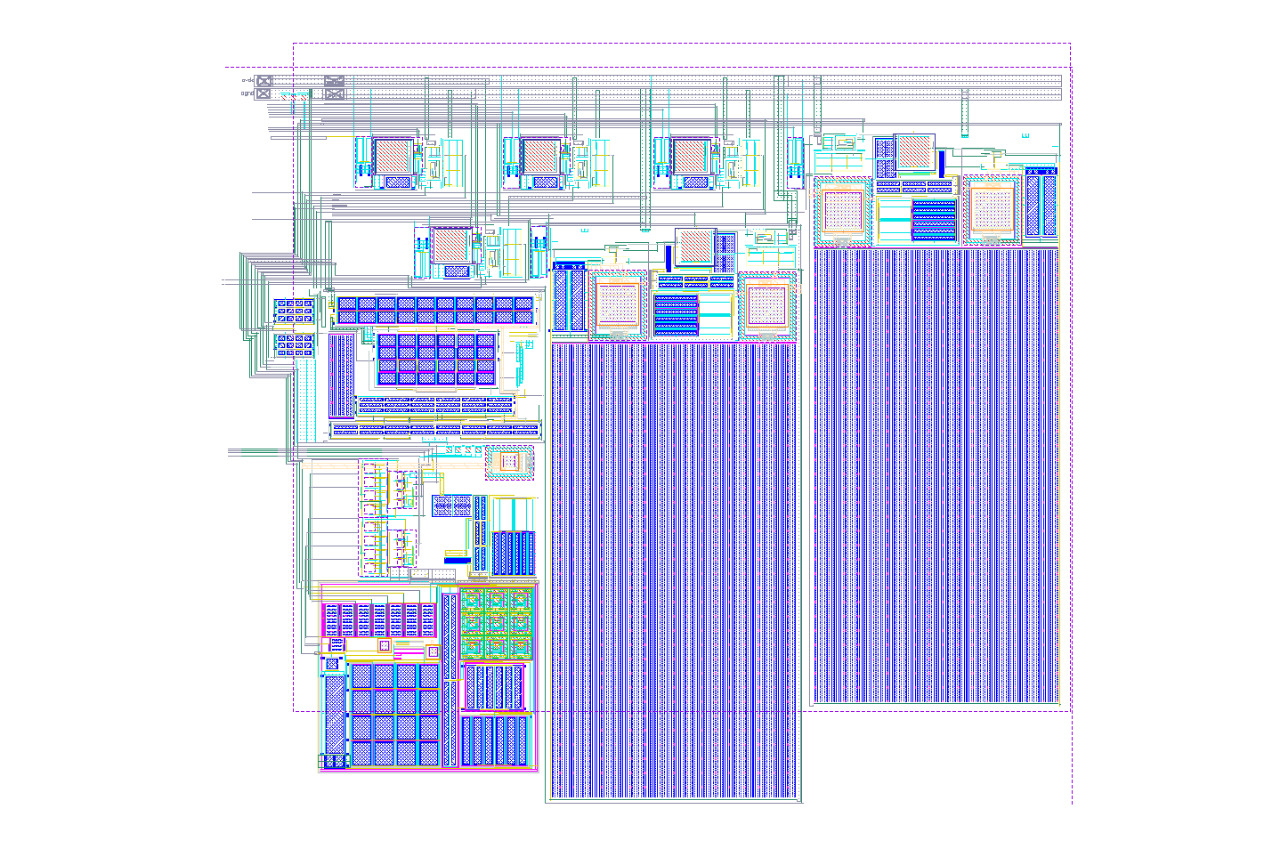
\includegraphics[scale=0.5, angle=90]{Resultados/Imagens/Circuito Completo.jpeg}
    \legend{Fonte: Produzido pelo autor}
    \nota{Imagem do circuito rotacionado em 90° em relação à orientação padrão do circuito no plano (1 1 0).}
\end{figure}


% ----------------------------------------------------------
% PARTE
% ----------------------------------------------------------

% ----------------------------------------------------------
% Finaliza a parte no bookmark do PDF
% para que se inicie o bookmark na raiz
% e adiciona espaço de parte no Sumário
% ----------------------------------------------------------
\phantompart

% ---
% Conclusão
% ---
\chapter{Conclusão}

O autor do trabalho apresentou a base teórica dos dispositivos APS e TIA, além das especificações de um projeto de Receptor Óptico, as soluções propostas pelo autor para o seu desenvolvimento, simulações para avaliação do dispositivo, e a elaboração do layout.

O projeto a nível de esquemático e o layout foi demonstrado para os principais blocos que compõem a solução proposta, com todos parâmetros de componentes especificados.

Simulações foram realizadas de forma a mostrar o funcionamento e viabilidade do dispositivo, que apresenta comportamento como esperado de toda teoria apresentada.

Com todo o trabalho aqui demonstrado, espera-se que o entendimento sobre o tema de Receptores Ópticos seja adequado para que o leitor possa replicar o projeto, adaptando-o para a aplicação que for direcionada, e que se possa realizar a validação do dispositivo de forma a demonstrar sua funcionalidade.

Desafios apareceram ao longo de todo o trabalho, tanto no entendimento da teoria por trás do tema, questões de desenvolvimento, projeto e simulação, dos quais necessitaram de ampla pesquisa acadêmica e também orientação para o seu devido entendimento e solução. Tudo demonstrado ao longo do trabalho veio de extensas tentativas do autor para possibilitar uma solução viável e que possa ser replicada. 

O trabalho como um todo teve seus objetivos alcançados, mostrando o desenvolvimento e simulação de um projeto de Receptor Óptico para três cores, e um circuito integrado foi desenvolvido para que seja realizado a sua validação.

\section{Trabalhos futuros}

O autor propõe que com a fabricação do circuito integrado, sejam realizadas todas as medições para validação do trabalho, e que este possa servir de conhecimento para outros que se proporem em estender o que foi aqui desenvolvido.

O tema pode ser expandido de forma a se validar outros Receptores Ópticos (como o \textit{CCD}), de forma a realizar uma comparação de diferentes tecnologias.
% ---

% ----------------------------------------------------------
% ELEMENTOS PÓS-TEXTUAIS
% ----------------------------------------------------------
\postextual
% ----------------------------------------------------------

% ----------------------------------------------------------
% Referências bibliográficas
% ----------------------------------------------------------
\bibliography{Referencias}


% ---
% Inicia os anexos
% ---
\begin{anexosenv}

% Imprime uma página indicando o início dos anexos
\partanexos

\chapter{Blocos Adicionais}
\label{blocosadicionais}

Alguns circuitos adicionais n\~ao foram diretamente especificados ao longo deste trabalho, por serem considerados pelo autor circuitos mais simples e com ampla flexibilidade de escolha de seus par\^ametros. Os projetos se deram de acordo com aproveitamento de circuitos j\'a existentes advindos de outros trabalhos disponibilizados pelo orientador ou ent\~ao previamente desenvolvidos pelo autor.

\renewcommand{\NomeBloco}{\emph{Inversor}}
\renewcommand{\NomeBlocoNoIt}{Inversor}
\renewcommand{\NomePTab}{tab_\NomeBlocoNoIt}
\renewcommand{\NomeSTab}{tab_\NomeBlocoNoIt2}
\renewcommand{\NomePFig}{fig_\NomeBlocoNoIt}
\renewcommand{\NomeSFig}{fig_\NomeBlocoNoIt2}
\renewcommand{\NomeTTab}{tab_\NomeBlocoNoIt3}

\section{\NomeBloco}
\label{inversor1}

O bloco \NomeBloco{} tem a finalidade de receber uma entrada digital, e colocar o n\'ivel l\'ogico invertido na sa\'ida. A \autoref{\NomePTab} indica a Tabela Verdade do bloco.

\begin{table}[htbp]

\caption{Tabela Verdade do bloco \NomeBloco}%
\label{\NomePTab}
\centering
\begin{tabular}{cc}
    \toprule
    Entrada & Saída \\
    \midrule \midrule
    0 & 1 \\
    \midrule
    1 & 0 \\
\bottomrule

\end{tabular}
\fonte{Produzido pelo autor.}
\end{table}

O bloco apresenta as defini{\c c}\~oes de sinais de entrada e sa\'ida referidos na \autoref{\NomeSTab}.

\begin{table}[htbp]
\caption{Sinais do bloco \NomeBloco}
\label{\NomeSTab}
\centering
\begin{tabular}{ccl}

    \toprule
    Sinal & Tipo    & Descri{\c c}\~ao        \\
    \midrule \midrule
    In    & Entrada & Sinal de Entrada \\
    \midrule
    Out   & Saída   & Sinal de Sa\'ida   \\
    \bottomrule
\end{tabular}
\legend{Fonte: Produzido pelo autor}
\end{table}

O circuito projetado para o bloco \'e demonstrado na \autoref{\NomePFig}.

\begin{figure}[htb]
 \label{NomePFig}
 \centering
  \begin{minipage}{0.4\textwidth}
    \centering
    \caption{Circuito CMOS projetado para o bloco \NomeBloco} \label{\NomePFig}
    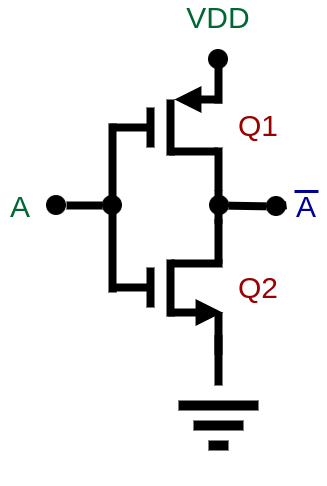
\includegraphics[scale=0.3]{Circuitos/NOT.png}
    \legend{Fonte: Produzido pelo autor}
  \end{minipage}
  \hfill
  \begin{minipage}{0.4\textwidth}
    \centering
    \caption{Representa{\c c}\~ao em bloco do \NomeBloco} \label{NomeSFig}
    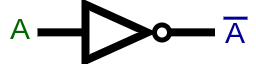
\includegraphics[scale=0.3]{Circuitos/NOT_block.png}
    \legend{Fonte: Produzido pelo autor}
  \end{minipage}
\end{figure}

Os transistores utilizados no bloco \NomeBloco{} apresentam os par\^ametros mostrados na \autoref{\NomeTTab}.

\begin{table}[htbp]
\caption{Transistores do Bloco \NomeBloco}
\label{\NomeTTab}
\centering
\begin{tabular}{ccccc}
\toprule
Transistor & W ($\mu$m)  & L ($\mu$m)           & M (n° dispositivos) & S (n° dispositivos)\\
\midrule \midrule
Q1 & 1,2 & 0,18 & 1 & 1\\
\midrule
Q2 & 0,6 & 0,18 & 1 & 1\\
\bottomrule
\end{tabular}
\legend{Fonte: Produzido pelo autor}
\end{table}
\renewcommand{\NomeBloco}{\emph{NAND}}
\renewcommand{\NomeBlocoNoIt}{NAND}
\renewcommand{\NomePTab}{tab_\NomeBlocoNoIt}
\renewcommand{\NomeSTab}{tab_\NomeBlocoNoIt2}
\renewcommand{\NomePFig}{fig_\NomeBlocoNoIt}
\renewcommand{\NomeSFig}{fig_\NomeBlocoNoIt2}
\renewcommand{\NomeTTab}{tab_\NomeBlocoNoIt3}

\subsection{\NomeBloco}
\label{inversor1}

O bloco \NomeBloco{} tem a finalidade de receber duas entradas digitais, e rcolocar o resultado da opera{\c c}\~ao NAND em sua sa\'ida. A \autoref{\NomePTab} indica a Tabela Verdade do bloco.

\begin{table}[htbp]

\caption{Tabela Verdade do bloco \NomeBloco}%
\label{\NomePTab}
\centering
\begin{tabular}{ccc}
\toprule
    A & B & Out \\
    \midrule \midrule
    0 & 0 & 1 \\
    \midrule
    0 & 1 & 1\\
    \midrule
    1 & 0 & 1\\
    \midrule
    1 & 1 & 0\\
\bottomrule

\end{tabular}
\fonte{Produzido pelo autor.}
\end{table}

O bloco apresenta as defini{\c c}\~oes de sinais de entrada e sa\'ida referidos na \autoref{\NomeSTab}.

\begin{table}[htbp]
\caption{Sinais do bloco \NomeBloco}
\label{\NomeSTab}
\centering
\begin{tabular}{ccl}

    \toprule
    Sinal & Tipo    & Descri{\c c}\~ao        \\
    \midrule \midrule
    A    & Entrada & Sinal de Entrada A \\
    \midrule
    B    & Entrada & Sinal de Entrada B \\
    \midrule
    Out    & Sa\'ida & Sinal de sa\'ida \\
    \bottomrule
\end{tabular}
\legend{Fonte: Produzido pelo autor}
\end{table}

O circuito projetado para o bloco \'e demonstrado na \autoref{\NomePFig}.

\begin{figure}[htbp]
 \label{NomePFig}
 \centering
  \begin{minipage}{0.4\textwidth}
    \centering
    \caption{Circuito CMOS projetado para o bloco \NomeBloco} \label{\NomePFig}
    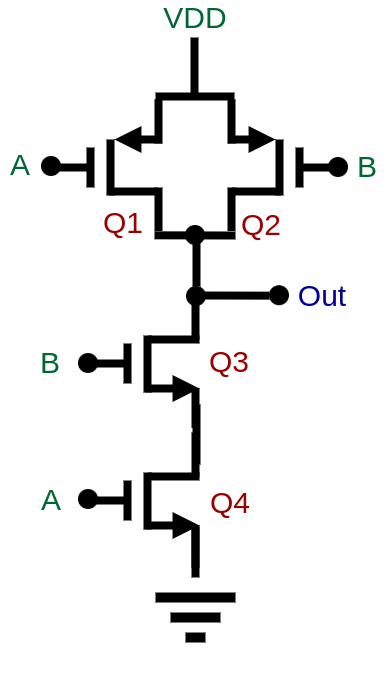
\includegraphics[scale=0.3]{Circuitos/NAND.png}
    \legend{Fonte: Produzido pelo autor}
  \end{minipage}
  \hfill
  \begin{minipage}{0.4\textwidth}
    \centering
    \caption{Representa{\c c}\~ao em bloco do \NomeBlocoNoIt} \label{NomeSFig}
    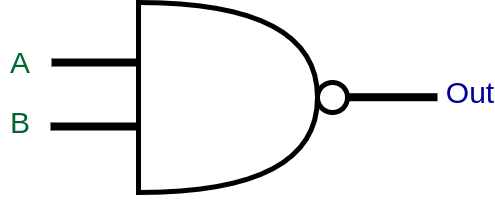
\includegraphics[scale=0.3]{Circuitos/NAND_block.png}
    \legend{Fonte: Produzido pelo autor}
  \end{minipage}
\end{figure}
\clearpage
\renewcommand{\NomeBloco}{\emph{Decoder 2x4}}
\renewcommand{\NomeBlocoNoIt}{Decoder 2x4}
\renewcommand{\NomePTab}{tab_\NomeBlocoNoIt}
\renewcommand{\NomeSTab}{tab_\NomeBlocoNoIt2}
\renewcommand{\NomePFig}{fig_\NomeBlocoNoIt}
\renewcommand{\NomeSFig}{fig_\NomeBlocoNoIt2}
\renewcommand{\NomeTTab}{tab_\NomeBlocoNoIt3}

\subsection{\NomeBloco}

O bloco \NomeBloco{} tem a fun{\c c}\~ao de colocar um bit '1' em uma das sa\'idas, enquanto todas outras s\~ao iguais a '0'. A \autoref{\NomePTab} indica a Tabela Verdade do bloco.

\begin{table}[htbp]

\caption{Tabela Verdade do bloco \NomeBloco}%
\label{\NomePTab}
\centering
\begin{tabular}{cccccc}
    \toprule
    In0 & In1 & Out0 & Out1 & Out2 & Out3 \\
    \midrule \midrule
    0 & 0 & 1 & 0 & 0 & 0 \\
    \midrule
    0 & 1 & 0 & 1 & 0 & 0 \\
    \midrule
    1 & 0 & 0 & 0 & 1 & 0 \\
    \midrule
    1 & 1 & 0 & 0 & 0 & 1 \\
\bottomrule

\end{tabular}
\fonte{Produzido pelo autor.}
\end{table}

O bloco apresenta as defini{\c c}\~oes de sinais de entrada e sa\'ida referidos na \autoref{\NomeSTab}.

\begin{table}[htbp]
\caption{Sinais do bloco \NomeBloco}
\label{\NomeSTab}
\centering
\begin{tabular}{ccl}

    \toprule
    Sinal & Tipo    & Descri{\c c}\~ao        \\
    \midrule \midrule
    In1    & Entrada & Primeira entrada de sele{\c c}\~ao de sa\'ida \\
    \midrule
    In2    & Entrada & Segunda entrada de sele{\c c}\~ao de sa\'ida \\
    \midrule
    Out0 & Sa\'ida & Sa\'ida 0\\
    \midrule
    Out1 & Sa\'ida & Sa\'ida 1\\
    \midrule
    Out2 & Sa\'ida & Sa\'ida 2\\
    \midrule
    Out3 & Sa\'ida & Sa\'ida 3\\
    \bottomrule
\end{tabular}
\legend{Fonte: Produzido pelo autor}
\end{table}

O circuito projetado para o bloco \'e demonstrado na \autoref{\NomePFig}.

\begin{figure}[htbp]
 \label{NomePFig}
 \centering
    \centering
    \caption{Circuito CMOS projetado para o bloco \NomeBloco} \label{\NomePFig}
    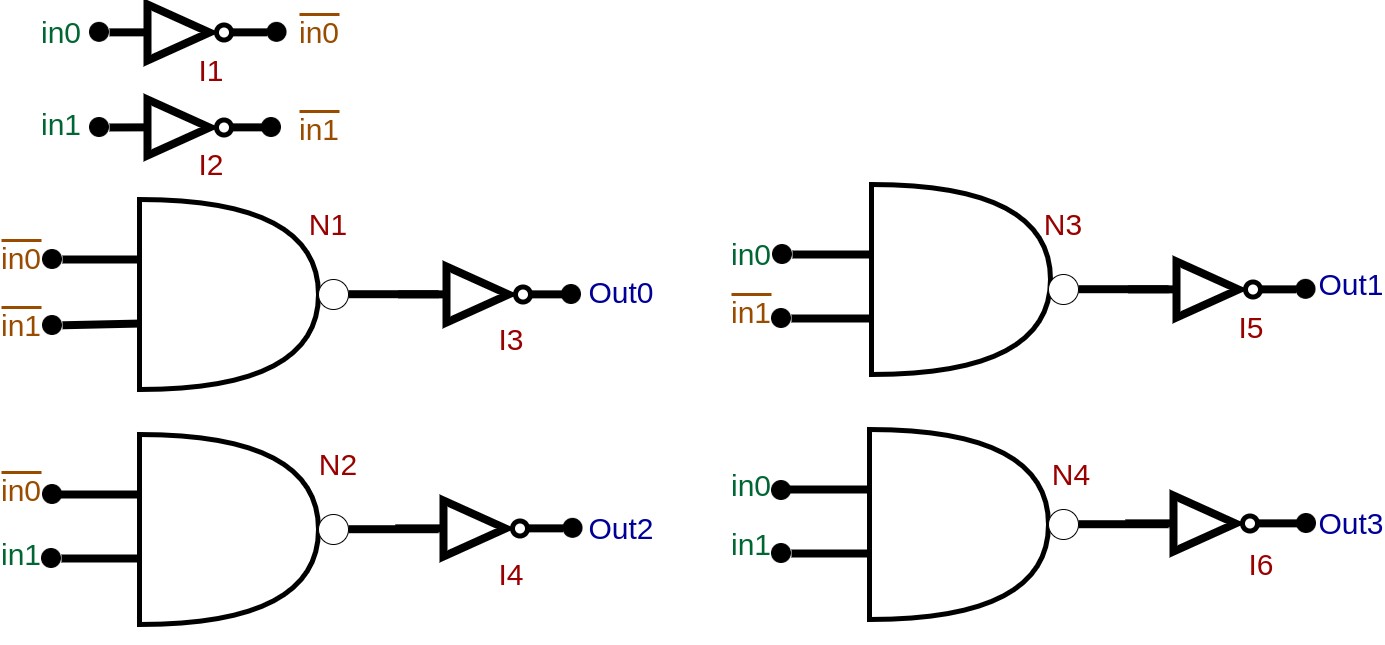
\includegraphics[scale=0.3]{Circuitos/decoder.png}
    \legend{Fonte: Produzido pelo autor}
\end{figure}

\begin{figure}[htbp]
 \label{NomeSFig}
 \centering
    \centering
    \caption{Representa{\c c}\~ao em bloco do \NomeBloco} \label{NomeSFig}
    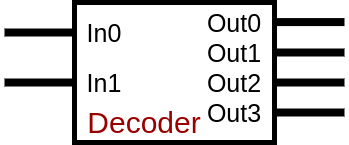
\includegraphics[scale=0.5]{Circuitos/decoder_block.png}
    \legend{Fonte: Produzido pelo autor}
\end{figure}
\clearpage
\renewcommand{\NomeBlocoNoIt}{\emph{Seletor 4x1}}
\renewcommand{\NomeBlocoNoIt}{Seletor 4x1}
\renewcommand{\NomePTab}{tab_\NomeBlocoNoIt}
\renewcommand{\NomeSTab}{tab_\NomeBlocoNoIt2}
\renewcommand{\NomePFig}{fig_\NomeBlocoNoIt}
\renewcommand{\NomeSFig}{fig_\NomeBlocoNoIt2}
\renewcommand{\NomeTTab}{tab_\NomeBlocoNoIt3}

O bloco \NomeBloco{} tem a finalidade de selecionar uma entrada, e a colocar na sa\'ida. A entrada \'e selecionada atrav\'es de 4 entradas de sele{\c c}\~ao, em que apenas uma deve estar em n\'ivel l\'ogico um por vez. A \autoref{\NomePTab} indica a Tabela Verdade do bloco. Embora tenha uma l\'ogica digital, o circuito permite entradas e sa\'idas anal\'ogicas.

\begin{table}[htbp]

\caption{Tabela Verdade do bloco \NomeBloco}%
\label{\NomePTab}
\centering
\begin{tabular}{ccccc}
    \toprule
    Sel1 & Sel2 & Sel3 & Sel4 & Out \\
    \midrule \midrule
    1 & 0 & 0 & 0 & In1 \\
    \midrule
    0 & 1 & 0 & 0 & In2 \\
    \midrule
    0 & 0 & 1 & 0 & In3 \\
    \midrule
    0 & 0 & 0 & 1 & In4 \\
    \midrule
    0 & 0 & 0 & 0 & Z \\
    \midrule
    X & X & X & X & X \\
\bottomrule

\end{tabular}
\fonte{Produzido pelo autor.}
\end{table}

O bloco apresenta as defini{\c c}\~oes de sinais de entrada e sa\'ida referidos na \autoref{\NomeSTab}.

\begin{table}[htbp]
\caption{Sinais do bloco \NomeBloco}
\label{\NomeSTab}
\centering
\begin{tabular}{ccl}

    \toprule
    Sinal & Tipo    & Descri{\c c}\~ao        \\
    \midrule \midrule
    In1    & Entrada & Primeira entrada \\
    \midrule
    Sel1    & Entrada & Sele{\c c}\~ao de entrada In1 \\
    \midrule
    In2    & Entrada & Segunda entrada \\
    \midrule
    Sel2    & Entrada & Sele{\c c}\~ao de entrada In2 \\
    \midrule
    In3    & Entrada & Terceira entrada \\
    \midrule
    Sel3    & Entrada & Sele{\c c}\~ao de entrada In3 \\
    \midrule
    In4    & Entrada & Quarta entrada \\
    \midrule
    Sel4    & Entrada & Sele{\c c}\~ao de entrada In4 \\
    \midrule
    Out   & Saída   & Sinal de Sa\'ida selecionado   \\
    \bottomrule
\end{tabular}
\legend{Fonte: Produzido pelo autor}
\end{table}

O circuito projetado para o bloco \'e demonstrado na \autoref{\NomePFig}.

\begin{figure}[htb]
 \label{NomePFig}
 \centering
    \centering
    \caption{Circuito CMOS projetado para o bloco \NomeBloco} \label{\NomePFig}
    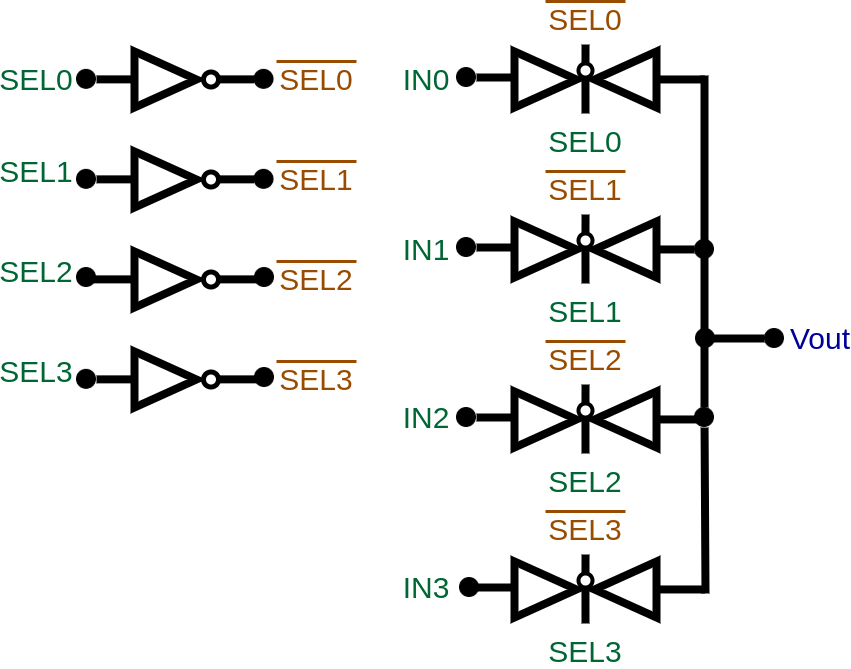
\includegraphics[scale=0.4]{Circuitos/sel4x1.png}
    \legend{Fonte: Produzido pelo autor}
\end{figure}

\begin{figure}[htb]
 \label{NomeSFig}
 \centering
    \centering
    \caption{Representa{\c c}\~ao em bloco do \NomeBloco} \label{NomeSFig}
    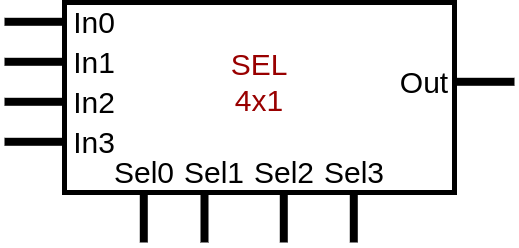
\includegraphics[scale=0.5]{Circuitos/sel4x1_block.png}
    \legend{Fonte: Produzido pelo autor}
\end{figure}

Os transistores utilizados no bloco \NomeBloco{} apresentam os par\^ametros mostrados na \autoref{\NomeTTab}.

\begin{table}[htbp]
\caption{Transistores do Bloco \NomeBloco}
\label{\NomeTTab}
\centering
\begin{tabular}{ccccc}
\toprule
Transistor & W ($\mu$m)  & L ($\mu$m)           & M (n° dispositivos) & S (n° dispositivos)\\
\midrule \midrule
Q1 & 1,2 & 0,18 & 1 & 1\\
\midrule
Q2 & 0,6 & 0,18 & 1 & 1\\
\bottomrule
\end{tabular}
\legend{Fonte: Produzido pelo autor}
\end{table}
\clearpage
\renewcommand{\NomeBloco}{\emph{Multiplexador 7x1}}
\renewcommand{\NomeBlocoNoIt}{Multiplexador 7x1}
\renewcommand{\NomePTab}{tab_\NomeBlocoNoIt}
\renewcommand{\NomeSTab}{tab_\NomeBlocoNoIt2}
\renewcommand{\NomePFig}{fig_\NomeBlocoNoIt}
\renewcommand{\NomeSFig}{fig_\NomeBlocoNoIt2}
\renewcommand{\NomeTTab}{tab_\NomeBlocoNoIt3}

\section{\NomeBloco}

O bloco \NomeBloco{} tem a fun{\c c}\~ao de colocar na sa\'ida o valor correspondente \'a entrada selecionada. Nesse bloco, 7 entradas distintas podem ser selecionadas. A \autoref{\NomePTab} indica a Tabela Verdade do bloco. Embora tenha uma l\'ogica digital, o circuito permite entradas e sa\'idas anal\'ogicas.

\begin{table}[htbp]

\caption{Tabela Verdade do bloco \NomeBloco}%
\label{\NomePTab}
\centering
\begin{tabular}{ccccc}
    \toprule
    D0 & D1 & D2 & D3 & Out \\
    \midrule \midrule
    0 & 0 & 0 & 0 & In0 \\
    \midrule
    0 & 1 & 0 & 0 & In1 \\
    \midrule
    1 & 0 & 0 & 0 & In2 \\
    \midrule
    1 & 1 & 0 & 0 & In3 \\
    \midrule
    X & X & 0 & 1 & In4 \\
    \midrule
    X & X & 1 & 0 & In5 \\
    \midrule
    X & X & 1 & 1 & In6 \\
\bottomrule

\end{tabular}
\fonte{Produzido pelo autor.}
\end{table}

O bloco apresenta as defini{\c c}\~oes de sinais de entrada e sa\'ida referidos na \autoref{\NomeSTab}.

\begin{table}[htbp]
\caption{Sinais do bloco \NomeBloco}
\label{\NomeSTab}
\centering
\begin{tabular}{ccl}

    \toprule
    Sinal & Tipo    & Descri{\c c}\~ao        \\
    \midrule \midrule
    D0    & Entrada & Primeira entrada de sele{\c c}\~ao de sa\'ida \\
    \midrule
    D1    & Entrada & Segunda entrada de sele{\c c}\~ao de sa\'ida \\
    \midrule
    D2    & Entrada & Segunda entrada de sele{\c c}\~ao de sa\'ida \\
    \midrule
    D3    & Entrada & Segunda entrada de sele{\c c}\~ao de sa\'ida \\
    \midrule
    Vout & Sa\'ida & Sa\'ida do Multiplexador\\
    \midrule
    \bottomrule
\end{tabular}
\legend{Fonte: Produzido pelo autor}
\end{table}

O circuito projetado para o bloco \'e demonstrado na \autoref{\NomePFig}.

\begin{figure}[htbp]
 \label{NomePFig}
 \centering
    \centering
    \caption{Circuito CMOS projetado para o bloco \NomeBloco} \label{\NomePFig}
    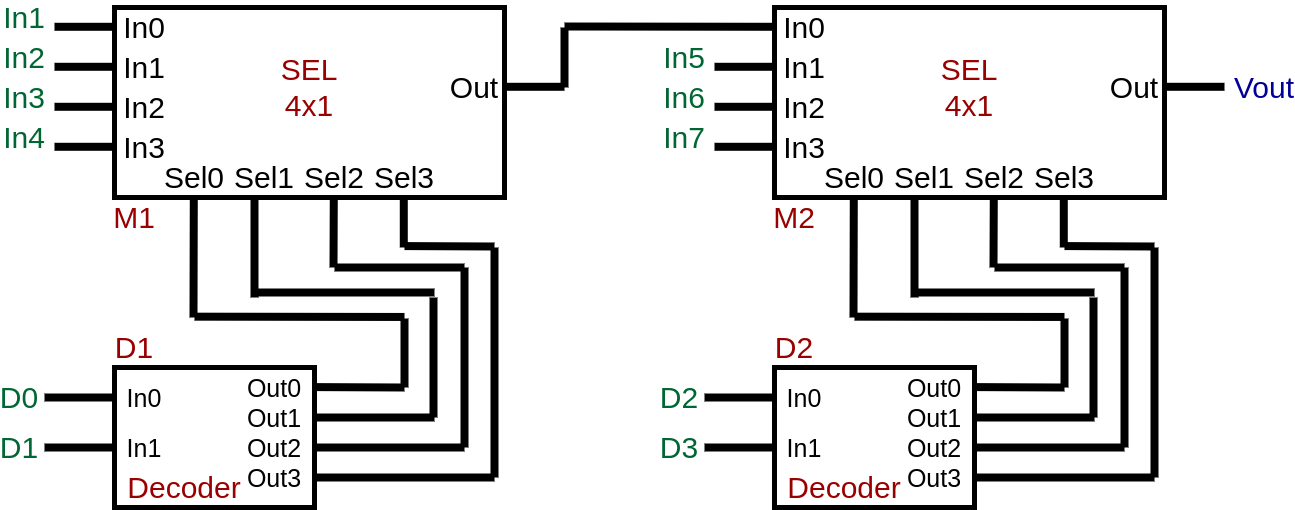
\includegraphics[scale=0.3]{Circuitos/mux7x1.png}
    \legend{Fonte: Produzido pelo autor}
\end{figure}

\begin{figure}[htbp]
 \label{NomeSFig}
 \centering
    \centering
    \caption{Representa{\c c}\~ao em bloco do \NomeBloco} \label{NomeSFig}
    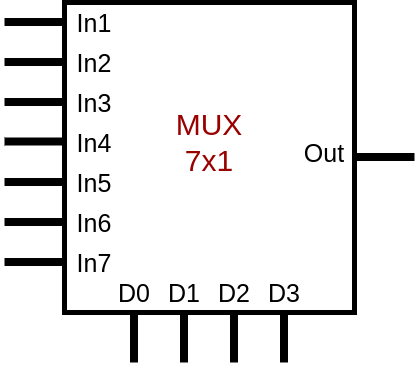
\includegraphics[scale=0.3]{Circuitos/mux7x1_block.png}
    \legend{Fonte: Produzido pelo autor}
\end{figure}
\renewcommand{\NomeBloco}{\emph{Porta de Transmissão}}
\renewcommand{\NomeBlocoNoIt}{Porta de Transmissão}
\renewcommand{\NomePTab}{tab_\NomeBlocoNoIt}
\renewcommand{\NomeSTab}{tab_\NomeBlocoNoIt2}
\renewcommand{\NomePFig}{fig_\NomeBlocoNoIt}
\renewcommand{\NomeSFig}{fig_\NomeBlocoNoIt2}
\renewcommand{\NomeTTab}{tab_\NomeBlocoNoIt3}

\subsection{\NomeBloco}

O bloco \emph{\NomeBloco{}} funciona como uma chave, permitindo ou n\~ao o sinal de um lado passar ao outro. O bloco apresenta as defini{\c c}\~oes de sinais de entrada e sa\'ida referidos na \autoref{\NomeSTab}.

\begin{table}[htbp]
\caption{Sinais do bloco \emph{\NomeBloco}}
\label{\NomeSTab}
\centering
\begin{tabular}{ccl}

    \toprule
    Sinal & Tipo    & Descri{\c c}\~ao        \\
    \midrule \midrule
    A & Bidirecional & Sinal bidirecional 1\\
    \midrule
    B & Bidirecional & Sinal bidirecional 2\\
    \midrule
    ENABLE & Entrada & Sinal de habilita{\c c}\~ao\\
    \bottomrule
\end{tabular}
\legend{Fonte: Produzido pelo autor}
\end{table}

O circuito projetado para o bloco \'e demonstrado na \autoref{\NomePFig}.

\begin{figure}[htb]
 \label{\NomePFig}
 \centering
  \begin{minipage}{0.4\textwidth}
    \centering
    \caption{Circuito CMOS projetado para o bloco \emph{\NomeBloco}} \label{\NomePFig}
    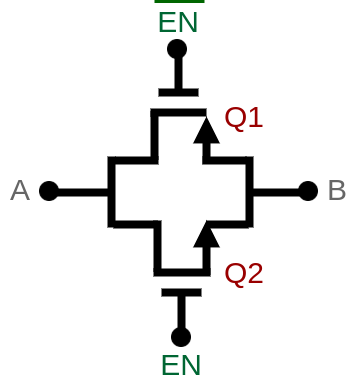
\includegraphics[scale=0.5]{Circuitos/TG.png}
    \legend{Fonte: Produzido pelo autor}
  \end{minipage}
  \hfill
  \begin{minipage}{0.4\textwidth}
    \centering
    \caption{Representa{\c c}\~ao em bloco do \emph{\NomeBloco}} \label{\NomeSFig}
    \includegraphics[scale=0.5]{Circuitos/TG_Simbolo.png}
    \legend{Fonte: Produzido pelo autor}
  \end{minipage}
\end{figure}

Os transistores utilizados no bloco \emph{\NomeBloco{}} apresentam os par\^ametros mostrados na \autoref{\NomeTTab}.

\begin{table}[htbp]
\caption{Transistores do Bloco \emph{\NomeBloco}}
\label{\NomeTTab}
\centering
\begin{tabular}{ccccc}
\toprule
Transistor & W ($\mu$m)  & L ($\mu$m)           & M (n° dispositivos) & S (n° dispositivos)\\
\midrule \midrule
Q1 & 0,8 & 0,18 & 1 & 1\\
\midrule
Q2 & 0,4 & 0,18 & 1 & 1\\
\bottomrule
\end{tabular}
\legend{Fonte: Produzido pelo autor}
\end{table}
\clearpage

\renewcommand{\NomeBloco}{Buffer}
\renewcommand{\NomePTab}{tab_\NomeBloco}
\renewcommand{\NomeSTab}{tab_\NomeBloco2}
\renewcommand{\NomePFig}{fig_\NomeBloco}
\renewcommand{\NomeSFig}{fig_\NomeBloco2}
\renewcommand{\NomeTTab}{tab_\NomeBloco3}

\section{Buffer}
\label{buffer}

O bloco \NomeBloco{} tem a finalidade de colocar o mesmo sinal de entrada na sua sa\'ida, reduzindo efeitos de carga. O sinal de entrada pode ser tanto anal\'ogico quanto digital. O bloco apresenta as definições de sinais de entrada e sa\'ida referidos na \autoref{\NomeSTab}.

\begin{table}[htb]
\caption{Sinais do bloco \NomeBloco}
\label{\NomeSTab}
\centering
\begin{tabular}{ccl}

    \toprule
    Sinal & Tipo    & Descrição        \\
    \midrule \midrule
    In    & Entrada & Sinal de Entrada \\
    \midrule
    Out   & Saída   & Sinal de Sa\'ida   \\
    \bottomrule
\end{tabular}
\legend{Fonte: Produzido pelo autor}
\end{table}

O circuito projetado para o bloco \'e demonstrado na \autoref{\NomePFig}.

\begin{figure}[htb]
 \centering
    \caption{\label{\NomePFig}Circuito CMOS projetado para o bloco \NomeBloco}
    \includegraphics[scale=0.3]{Circuitos/Buffer.png}
    \legend{Fonte: Produzido pelo autor}
\end{figure}

\begin{figure}[htb]
 \centering
    \centering
    \caption{Representação em bloco do \NomeBloco} \label{\NomeSFig2}
    \includegraphics[scale=0.3]{Circuitos/Buffer_block.png}
    \legend{Fonte: Produzido pelo autor}
\end{figure}


Os transistores utilizados no bloco \NomeBloco{} apresentam os par\^ametros mostrados na \autoref{\NomeTTab}.

\begin{table}[htb]
\caption{Transistores do Bloco \NomeBloco}
\label{\NomeTTab}
\centering
\begin{tabular}{ccccc}
\toprule
Transistor & W ($\mu$m)  & L ($\mu$m)           & M (n° dispositivos) & S (n° dispositivos)\\
\midrule \midrule
Q1 e Q6 & 0,22 & 0,54 & 1 & 1\\
\midrule
Q2 e Q7 & 0,66 & 0,54 & 1 & 1\\
\midrule
Q3 e Q8 & 1,98 & 0,54 & 1 & 1\\
\midrule
Q4 e Q9 & 5,94 & 0,54 & 1 & 1\\
\midrule
Q5 e Q10 & 17,82 & 0,54 & 1 & 1\\
\bottomrule
\end{tabular}
\legend{Fonte: Produzido pelo autor}
\end{table}
\renewcommand{\NomeBloco}{\emph{Par Diferencial}}
\renewcommand{\NomeBlocoNoIt}{Par Diferencial}
\renewcommand{\NomePTab}{tab_\NomeBlocoNoIt}
\renewcommand{\NomeSTab}{tab_\NomeBlocoNoIt2}
\renewcommand{\NomePFig}{fig_\NomeBlocoNoIt}
\renewcommand{\NomeSFig}{fig_\NomeBlocoNoIt2}
\renewcommand{\NomeTTab}{tab_\NomeBlocoNoIt3}
\renewcommand{\NomeQTab}{tab_\NomeBlocoNoIt4}

\section{\NomeBloco}

O bloco \NomeBloco{} tem a mesma fun{\c c}\~ao de comparar duas entradas, fazendo a diferença entre elas, e colocar o resultado vezes um ganho na saída. O bloco apresenta as defini{\c c}\~oes de sinais de entrada e sa\'ida referidos na \autoref{\NomeSTab}.

\begin{table}[htbp]
\caption{Sinais do bloco \NomeBloco}
\label{\NomeSTab}
\centering
\begin{tabular}{ccl}

    \toprule
    Sinal & Tipo    & Descri{\c c}\~ao        \\
    \midrule \midrule
    Vp (+) & Entrada & Entrada positiva do Comparador\\
    \midrule
    Vn (-) & Entrada & Entrada negativa do Comparador\\
    \midrule
    Ibias & Entrada & Corrente de polariza{\c c}\~ao do Comparador\\
    \midrule
    Vo & sa\'ida & Sa\'ida do Comparador\\
    \bottomrule
\end{tabular}
\legend{Fonte: Produzido pelo autor}
\end{table}

O circuito projetado para o bloco \'e demonstrado na \autoref{\NomePFig}.

\begin{figure}[htb]
 \label{\NomePFig}
 \centering
    \centering
    \caption{Circuito CMOS projetado para o bloco \NomeBloco} 
    \includegraphics[scale=0.4]{Circuitos/diff_pair.png}
    \legend{Fonte: Produzido pelo autor}
\end{figure}

\begin{figure}[htb]
 \centering
    \centering
    \caption{Representa{\c c}\~ao em bloco do \NomeBloco} \label{\NomeSFig}
    \includegraphics[scale=0.3]{Circuitos/diff_pair_block.png}
    \legend{Fonte: Produzido pelo autor}
\end{figure}

Os transistores utilizados no bloco \NomeBloco{} apresentam os par\^ametros mostrados na \autoref{\NomeTTab}.

\begin{table}[htbp]
\caption{Transistores do Bloco \NomeBloco}
\label{\NomeTTab}
\centering
\begin{tabular}{ccccc}
\toprule
Transistor & W ($\mu$m)  & L ($\mu$m)           & M (n° dispositivos) & S (n° dispositivos)\\
\midrule \midrule
Q1 e Q2 & 40 & 7 & 2 & 1\\
\midrule
Q3 e Q4 & 35 & 6 & 2 & 1\\
\midrule
Q5 e Q6¹ & 70 & 4 & 1 & 1\\

\bottomrule
\end{tabular}
\legend{Fonte: Produzido pelo autor}
\legend{$^1$Calculado de forma a produzir uma corrente de 50 $\mu$A}
\end{table}

Um segundo circuito, chamado de \emph{diff\_3} de mesma topologia apresentado na \autoref{\NomePFig} foi desenvolvido, por\'em com par\^ametros distintos, dados na \autoref{pard_diff3}.

\begin{figure}[htb]
 \centering
    \centering
    \caption{Representa{\c c}\~ao em bloco do diff\_3} \label{\NomeSFig}
    \includegraphics[scale=0.3]{Circuitos/diff_pair_3_block.png}
    \legend{Fonte: Produzido pelo autor}
\end{figure}

\begin{table}[htbp]
\caption{Transistores do Bloco diff\_pair\_3}
\label{pard_diff3}
\centering
\begin{tabular}{ccccc}
\toprule
Transistor & W ($\mu$m)  & L ($\mu$m)           & M (n° dispositivos) & S (n° dispositivos)\\
\midrule \midrule
Q1 e Q2 & 10 & 0.5 & 2 & 1\\
\midrule
Q3 e Q4 & 5 & 0.5 & 2 & 1\\
\midrule
Q5 e Q6¹ & 50 & 3 & 2 & 1\\

\bottomrule
\end{tabular}
\legend{Fonte: Produzido pelo autor}
\legend{$^1$Calculado de forma a produzir uma corrente de 50 $\mu$A}
\end{table}
\label{anexoespelhos}

\section{Espelho de Corrente NMOS}

Um espelho de corrente \'e um circuito que replica o sinal de uma corrente de refer\^encia em outras sa\'idas, podendo ser multiplicado por um fator de ajuste. A \autoref{fig_espelho} mostra a representa ção de um circuito com tal caracter\'istica, utilizando transistores NMOS. O espelho de corrente NMOS tamb\'em \'e chamado de dreno de corrente, por drenar a corrente nos ramos.

\begin{figure}[htb]
    \label{fig_espelho}
    \centering
    \caption{Espelho de corrente NMOS} 
    \includegraphics[scale=0.4]{Circuitos/current_mirror_example.png}
    \legend{Fonte: Produzido pelo autor}
\end{figure}

Nesta figura, est\'a representado a utiliza ção de uma corrente de refer\^encia Iref para gerar as correntes Io1, Io2 at\'e Ion, onde "n" \'e o n\'umero de transistores se referenciando por $Q_{ref}$.

No circuito demonstrado pela \autoref{fig_espelho}, o transistor \emph{Qref} tem funç\^ao de captar a corrente igual \'a \emph{Iref}, para servir de refer\^encia aos outros transistores \emph{Q1}, \emph{Q2} at\'e \emph{Qn}, onde \emph{n} \'e o numero de transistores que se referenciam de Q\_ref, e que são chamados de bra ços do espelho. O potencial \emph{VDD\_IREF} \'e um valor de tensão utilizado para polarizar Iref, que não precisa ser igual ao valor de alimenta ção dos outros bra ços.

Dado o parâmetro $W_x/L_x$ de cada transistor, onde "x" é o número indicado do transistor, podemos calcular o valor de corrente de cada braço utilizando a fórmula apresentada na \autoref{eq_espcorpmos}.

\begin{equation}
    \label{eq_espcor}
    I_{OX} = Iref\frac{W_x/L_x}{W_{ref}/L_{ref}}
\end{equation}

Onde $I{ox}$ \'e a corrente de entrada do bra ço \emph{Qx}. 

Para que esse circuito funcione devidamente em cada sa\'ida, cada bra ço do espelho deve estar necessariamente operando na região ativa, pois a \autoref{eq_espcor} \'e deduzida levando isso em conta. Para que isso aconte ça, devemos respeitar a \autoref{eq_curmirror_req} \cite{RazaviFundM}.

\begin{equation}
    \label{eq_curmirror_req}
    v_{DS} \geq v_{GS} - V_t
\end{equation}

Onde:

\begin{itemize}
    \item $v_{DS}$ \'e a tensão entre o dreno e fonte do transistor
    \item $v_{GS}$ \'e a tensão entre o porta e fonte do transistor
    \item $V_{t}$ \'e a tensão de limiar do transistor
\end{itemize}

\section{Espelho de Corrente PMOS}

Um circuito de espelho de corrente pode ser constru\'ido com transistores PMOS, utilizando o mesmo racioc\'inio de constru ção do circuito NMOS, conforme a \autoref{fig_curmir_pmos}. A diferen ça principal \'e que em vez de ser um dreno de corrente, o PMOS ser\'a um fornecedor de corrente.

\begin{figure}[htb]
    \label{fig_curmir_pmos}
    \centering
    \caption{Espelho de corrente PMOS} 
    \includegraphics[scale=0.4]{Circuitos/current_mirror_example_pmos.png}
    \legend{Fonte: Produzido pelo autor}
\end{figure}

O funcionamento do circuito PMOS segue o mesmo principio do NMOS, porém, ao inv\'es de receber corrente fixada a um n\'o, ele fornece. O potencial \emph{negVDD\_{IREF}} \'e um valor de tensão utilizado para polarizar Iref, que não precisa ser igual ao valor de alimenta ção negativa/terra dos outros bra ços.

Dado o parâmetro $W_x/L_x$ de cada transistor, onde "x" é o número indicado do transistor, podemos calcular o valor de corrente de cada braço utilizando a fórmula apresentada na \autoref{eq_espcorpmos}.

\begin{equation}
    \label{eq_espcorpmos}
    I_{OX} = I_{ref}\frac{W_x/L_x}{W_{ref}/L_{ref}}
\end{equation}

Onde $I_{OX}$ \'e a corrente de sa\'ida do bra ço \emph{Qx}. 

Assim como no caso do NMOS, todos transistores devem estar na região ativa, e respeitar a seguinte \autoref{eq_curmirror_reqpmos} \cite{RazaviFundM}.

\begin{equation}
    \label{eq_curmirror_reqpmos}
    v_{SD} \geq v_{SG} - |V_t|
\end{equation}

Onde:

\begin{itemize}
    \item $v_{SD}$ \'e a tensão entre o fonte e dreno do transistor
    \item $v_{SG}$ \'e a tensão entre a fonte e oirta do transistor
    \item $V_{t}$ \'e a tensão de limiar do transistor
\end{itemize}



\end{anexosenv}

% ----------------------------------------------------------
% Glossário
% ----------------------------------------------------------
%
% Consulte o manual da classe abntex2 para orientações sobre o glossário.
%
%\glossary

%---------------------------------------------------------------------
% INDICE REMISSIVO
%---------------------------------------------------------------------
\phantompart
\printindex
%---------------------------------------------------------------------

\end{document}
